\documentclass[twoside]{book}

% Packages required by doxygen
\usepackage{fixltx2e}
\usepackage{calc}
\usepackage{doxygen}
\usepackage[export]{adjustbox} % also loads graphicx
\usepackage{graphicx}
\usepackage[utf8]{inputenc}
\usepackage{makeidx}
\usepackage{multicol}
\usepackage{multirow}
\PassOptionsToPackage{warn}{textcomp}
\usepackage{textcomp}
\usepackage[nointegrals]{wasysym}
\usepackage[table]{xcolor}

% Font selection
\usepackage[T1]{fontenc}
\usepackage[scaled=.90]{helvet}
\usepackage{courier}
\usepackage{amssymb}
\usepackage{sectsty}
\renewcommand{\familydefault}{\sfdefault}
\allsectionsfont{%
  \fontseries{bc}\selectfont%
  \color{darkgray}%
}
\renewcommand{\DoxyLabelFont}{%
  \fontseries{bc}\selectfont%
  \color{darkgray}%
}
\newcommand{\+}{\discretionary{\mbox{\scriptsize$\hookleftarrow$}}{}{}}

% Page & text layout
\usepackage{geometry}
\geometry{%
  a4paper,%
  top=2.5cm,%
  bottom=2.5cm,%
  left=2.5cm,%
  right=2.5cm%
}
\tolerance=750
\hfuzz=15pt
\hbadness=750
\setlength{\emergencystretch}{15pt}
\setlength{\parindent}{0cm}
\setlength{\parskip}{3ex plus 2ex minus 2ex}
\makeatletter
\renewcommand{\paragraph}{%
  \@startsection{paragraph}{4}{0ex}{-1.0ex}{1.0ex}{%
    \normalfont\normalsize\bfseries\SS@parafont%
  }%
}
\renewcommand{\subparagraph}{%
  \@startsection{subparagraph}{5}{0ex}{-1.0ex}{1.0ex}{%
    \normalfont\normalsize\bfseries\SS@subparafont%
  }%
}
\makeatother

% Headers & footers
\usepackage{fancyhdr}
\pagestyle{fancyplain}
\fancyhead[LE]{\fancyplain{}{\bfseries\thepage}}
\fancyhead[CE]{\fancyplain{}{}}
\fancyhead[RE]{\fancyplain{}{\bfseries\leftmark}}
\fancyhead[LO]{\fancyplain{}{\bfseries\rightmark}}
\fancyhead[CO]{\fancyplain{}{}}
\fancyhead[RO]{\fancyplain{}{\bfseries\thepage}}
\fancyfoot[LE]{\fancyplain{}{}}
\fancyfoot[CE]{\fancyplain{}{}}
\fancyfoot[RE]{\fancyplain{}{\bfseries\scriptsize Generated by Doxygen }}
\fancyfoot[LO]{\fancyplain{}{\bfseries\scriptsize Generated by Doxygen }}
\fancyfoot[CO]{\fancyplain{}{}}
\fancyfoot[RO]{\fancyplain{}{}}
\renewcommand{\footrulewidth}{0.4pt}
\renewcommand{\chaptermark}[1]{%
  \markboth{#1}{}%
}
\renewcommand{\sectionmark}[1]{%
  \markright{\thesection\ #1}%
}

% Indices & bibliography
\usepackage{natbib}
\usepackage[titles]{tocloft}
\setcounter{tocdepth}{3}
\setcounter{secnumdepth}{5}
\makeindex

% Hyperlinks (required, but should be loaded last)
\usepackage{ifpdf}
\ifpdf
  \usepackage[pdftex,pagebackref=true]{hyperref}
\else
  \usepackage[ps2pdf,pagebackref=true]{hyperref}
\fi
\hypersetup{%
  colorlinks=true,%
  linkcolor=blue,%
  citecolor=blue,%
  unicode%
}

% Custom commands
\newcommand{\clearemptydoublepage}{%
  \newpage{\pagestyle{empty}\cleardoublepage}%
}

\usepackage{caption}
\captionsetup{labelsep=space,justification=centering,font={bf},singlelinecheck=off,skip=4pt,position=top}

%===== C O N T E N T S =====

\begin{document}

% Titlepage & ToC
\hypersetup{pageanchor=false,
             bookmarksnumbered=true,
             pdfencoding=unicode
            }
\pagenumbering{alph}
\begin{titlepage}
\vspace*{7cm}
\begin{center}%
{\Large Computer Graphics }\\
\vspace*{1cm}
{\large Generated by Doxygen 1.8.12}\\
\end{center}
\end{titlepage}
\clearemptydoublepage
\pagenumbering{roman}
\tableofcontents
\clearemptydoublepage
\pagenumbering{arabic}
\hypersetup{pageanchor=true}

%--- Begin generated contents ---
\chapter{Namespace Index}
\section{Namespace List}
Here is a list of all namespaces with brief descriptions\+:\begin{DoxyCompactList}
\item\contentsline{section}{\hyperlink{namespace_g_l_s_l_shader}{G\+L\+S\+L\+Shader} }{\pageref{namespace_g_l_s_l_shader}}{}
\item\contentsline{section}{\hyperlink{namespace_ui}{Ui} }{\pageref{namespace_ui}}{}
\end{DoxyCompactList}

\chapter{Hierarchical Index}
\section{Class Hierarchy}
This inheritance list is sorted roughly, but not completely, alphabetically\+:\begin{DoxyCompactList}
\item \contentsline{section}{G\+L\+S\+L\+Program}{\pageref{class_g_l_s_l_program}}{}
\item \contentsline{section}{G\+L\+Utils}{\pageref{class_g_l_utils}}{}
\item Q\+Dialog\begin{DoxyCompactList}
\item \contentsline{section}{Dialog}{\pageref{class_dialog}}{}
\item \contentsline{section}{Dialog\+Eyes}{\pageref{class_dialog_eyes}}{}
\end{DoxyCompactList}
\item Q\+G\+L\+Widget\begin{DoxyCompactList}
\item \contentsline{section}{Main\+View}{\pageref{class_main_view}}{}
\end{DoxyCompactList}
\item Q\+Main\+Window\begin{DoxyCompactList}
\item \contentsline{section}{Main\+Window}{\pageref{class_main_window}}{}
\end{DoxyCompactList}
\item \contentsline{section}{qt\+\_\+meta\+\_\+stringdata\+\_\+\+Dialog\+\_\+t}{\pageref{structqt__meta__stringdata___dialog__t}}{}
\item \contentsline{section}{qt\+\_\+meta\+\_\+stringdata\+\_\+\+Dialog\+\_\+view\+\_\+t}{\pageref{structqt__meta__stringdata___dialog__view__t}}{}
\item \contentsline{section}{qt\+\_\+meta\+\_\+stringdata\+\_\+\+Dialog\+Eyes\+\_\+t}{\pageref{structqt__meta__stringdata___dialog_eyes__t}}{}
\item \contentsline{section}{qt\+\_\+meta\+\_\+stringdata\+\_\+\+Main\+View\+\_\+t}{\pageref{structqt__meta__stringdata___main_view__t}}{}
\item \contentsline{section}{qt\+\_\+meta\+\_\+stringdata\+\_\+\+Main\+Window\+\_\+t}{\pageref{structqt__meta__stringdata___main_window__t}}{}
\item \contentsline{section}{Scene}{\pageref{class_scene}}{}
\begin{DoxyCompactList}
\item \contentsline{section}{Scene\+Basic}{\pageref{class_scene_basic}}{}
\end{DoxyCompactList}
\item \contentsline{section}{Set\+Of\+Values}{\pageref{struct_set_of_values}}{}
\item \contentsline{section}{set\+Of\+Values}{\pageref{structset_of_values}}{}
\item \contentsline{section}{Set\+Of\+View}{\pageref{struct_set_of_view}}{}
\item \contentsline{section}{set\+Of\+View}{\pageref{structset_of_view}}{}
\item \contentsline{section}{Ui\+\_\+\+Dialog}{\pageref{class_ui___dialog}}{}
\begin{DoxyCompactList}
\item \contentsline{section}{Ui\+:\+:Dialog}{\pageref{class_ui_1_1_dialog}}{}
\end{DoxyCompactList}
\item \contentsline{section}{Ui\+\_\+\+Dialog\+\_\+view}{\pageref{class_ui___dialog__view}}{}
\begin{DoxyCompactList}
\item \contentsline{section}{Ui\+:\+:Dialog\+\_\+view}{\pageref{class_ui_1_1_dialog__view}}{}
\end{DoxyCompactList}
\item \contentsline{section}{Ui\+\_\+\+Dialog\+Eyes}{\pageref{class_ui___dialog_eyes}}{}
\begin{DoxyCompactList}
\item \contentsline{section}{Ui\+:\+:Dialog\+Eyes}{\pageref{class_ui_1_1_dialog_eyes}}{}
\end{DoxyCompactList}
\item \contentsline{section}{Ui\+\_\+\+Main\+Window}{\pageref{class_ui___main_window}}{}
\begin{DoxyCompactList}
\item \contentsline{section}{Ui\+:\+:Main\+Window}{\pageref{class_ui_1_1_main_window}}{}
\end{DoxyCompactList}
\end{DoxyCompactList}

\chapter{Class Index}
\section{Class List}
Here are the classes, structs, unions and interfaces with brief descriptions\+:\begin{DoxyCompactList}
\item\contentsline{section}{\hyperlink{class_dialog}{Dialog} \\*Set the structure and the links between objects when parameters of the line are entered }{\pageref{class_dialog}}{}
\item\contentsline{section}{\hyperlink{class_ui_1_1_dialog}{Ui\+::\+Dialog} }{\pageref{class_ui_1_1_dialog}}{}
\item\contentsline{section}{\hyperlink{class_ui_1_1_dialog__view}{Ui\+::\+Dialog\+\_\+view} }{\pageref{class_ui_1_1_dialog__view}}{}
\item\contentsline{section}{\hyperlink{class_dialog_eyes}{Dialog\+Eyes} \\*Set the structure and the links between objects when parameters of the view are entered }{\pageref{class_dialog_eyes}}{}
\item\contentsline{section}{\hyperlink{class_ui_1_1_dialog_eyes}{Ui\+::\+Dialog\+Eyes} }{\pageref{class_ui_1_1_dialog_eyes}}{}
\item\contentsline{section}{\hyperlink{class_g_l_s_l_program}{G\+L\+S\+L\+Program} }{\pageref{class_g_l_s_l_program}}{}
\item\contentsline{section}{\hyperlink{class_g_l_utils}{G\+L\+Utils} }{\pageref{class_g_l_utils}}{}
\item\contentsline{section}{\hyperlink{class_main_view}{Main\+View} \\*It is the main view, it will recover data and transmit them }{\pageref{class_main_view}}{}
\item\contentsline{section}{\hyperlink{class_ui_1_1_main_window}{Ui\+::\+Main\+Window} }{\pageref{class_ui_1_1_main_window}}{}
\item\contentsline{section}{\hyperlink{class_main_window}{Main\+Window} \\*It is the main window, where the user can choose parameters }{\pageref{class_main_window}}{}
\item\contentsline{section}{\hyperlink{structqt__meta__stringdata___dialog__t}{qt\+\_\+meta\+\_\+stringdata\+\_\+\+Dialog\+\_\+t} }{\pageref{structqt__meta__stringdata___dialog__t}}{}
\item\contentsline{section}{\hyperlink{structqt__meta__stringdata___dialog__view__t}{qt\+\_\+meta\+\_\+stringdata\+\_\+\+Dialog\+\_\+view\+\_\+t} }{\pageref{structqt__meta__stringdata___dialog__view__t}}{}
\item\contentsline{section}{\hyperlink{structqt__meta__stringdata___dialog_eyes__t}{qt\+\_\+meta\+\_\+stringdata\+\_\+\+Dialog\+Eyes\+\_\+t} }{\pageref{structqt__meta__stringdata___dialog_eyes__t}}{}
\item\contentsline{section}{\hyperlink{structqt__meta__stringdata___main_view__t}{qt\+\_\+meta\+\_\+stringdata\+\_\+\+Main\+View\+\_\+t} }{\pageref{structqt__meta__stringdata___main_view__t}}{}
\item\contentsline{section}{\hyperlink{structqt__meta__stringdata___main_window__t}{qt\+\_\+meta\+\_\+stringdata\+\_\+\+Main\+Window\+\_\+t} }{\pageref{structqt__meta__stringdata___main_window__t}}{}
\item\contentsline{section}{\hyperlink{class_scene}{Scene} }{\pageref{class_scene}}{}
\item\contentsline{section}{\hyperlink{class_scene_basic}{Scene\+Basic} \\*It is the scene of the project. Where all transformations, actions are done }{\pageref{class_scene_basic}}{}
\item\contentsline{section}{\hyperlink{struct_set_of_values}{Set\+Of\+Values} }{\pageref{struct_set_of_values}}{}
\item\contentsline{section}{\hyperlink{structset_of_values}{set\+Of\+Values} }{\pageref{structset_of_values}}{}
\item\contentsline{section}{\hyperlink{struct_set_of_view}{Set\+Of\+View} }{\pageref{struct_set_of_view}}{}
\item\contentsline{section}{\hyperlink{structset_of_view}{set\+Of\+View} }{\pageref{structset_of_view}}{}
\item\contentsline{section}{\hyperlink{class_ui___dialog}{Ui\+\_\+\+Dialog} }{\pageref{class_ui___dialog}}{}
\item\contentsline{section}{\hyperlink{class_ui___dialog__view}{Ui\+\_\+\+Dialog\+\_\+view} }{\pageref{class_ui___dialog__view}}{}
\item\contentsline{section}{\hyperlink{class_ui___dialog_eyes}{Ui\+\_\+\+Dialog\+Eyes} }{\pageref{class_ui___dialog_eyes}}{}
\item\contentsline{section}{\hyperlink{class_ui___main_window}{Ui\+\_\+\+Main\+Window} }{\pageref{class_ui___main_window}}{}
\end{DoxyCompactList}

\chapter{File Index}
\section{File List}
Here is a list of all files with brief descriptions\+:\begin{DoxyCompactList}
\item\contentsline{section}{D\+:/\+Q\+T\+\_\+projets/\+Cube\+Menu/\hyperlink{dialog_8cpp}{dialog.\+cpp} }{\pageref{dialog_8cpp}}{}
\item\contentsline{section}{D\+:/\+Q\+T\+\_\+projets/\+Cube\+Menu/\hyperlink{dialog_8h}{dialog.\+h} \\*Graphical user interface when the user set parameters of the line and of the angle of rotation }{\pageref{dialog_8h}}{}
\item\contentsline{section}{D\+:/\+Q\+T\+\_\+projets/\+Cube\+Menu/\hyperlink{dialogeyes_8cpp}{dialogeyes.\+cpp} }{\pageref{dialogeyes_8cpp}}{}
\item\contentsline{section}{D\+:/\+Q\+T\+\_\+projets/\+Cube\+Menu/\hyperlink{dialogeyes_8h}{dialogeyes.\+h} \\*Graphical user interface when the user set parameters of the camera }{\pageref{dialogeyes_8h}}{}
\item\contentsline{section}{D\+:/\+Q\+T\+\_\+projets/\+Cube\+Menu/\hyperlink{glslprogram_8cpp}{glslprogram.\+cpp} }{\pageref{glslprogram_8cpp}}{}
\item\contentsline{section}{D\+:/\+Q\+T\+\_\+projets/\+Cube\+Menu/\hyperlink{glslprogram_8h}{glslprogram.\+h} \\*All functions and ways to load, create, compile shaders, apply transformations etc .. It is the link whit the graphical card }{\pageref{glslprogram_8h}}{}
\item\contentsline{section}{D\+:/\+Q\+T\+\_\+projets/\+Cube\+Menu/\hyperlink{glutils_8cpp}{glutils.\+cpp} }{\pageref{glutils_8cpp}}{}
\item\contentsline{section}{D\+:/\+Q\+T\+\_\+projets/\+Cube\+Menu/\hyperlink{glutils_8h}{glutils.\+h} \\*Management of possible errors }{\pageref{glutils_8h}}{}
\item\contentsline{section}{D\+:/\+Q\+T\+\_\+projets/\+Cube\+Menu/\hyperlink{main_8cpp}{main.\+cpp} }{\pageref{main_8cpp}}{}
\item\contentsline{section}{D\+:/\+Q\+T\+\_\+projets/\+Cube\+Menu/\hyperlink{mainview_8cpp}{mainview.\+cpp} }{\pageref{mainview_8cpp}}{}
\item\contentsline{section}{D\+:/\+Q\+T\+\_\+projets/\+Cube\+Menu/\hyperlink{mainview_8h}{mainview.\+h} \\*Main view, link choices made by the user with actions inside the code }{\pageref{mainview_8h}}{}
\item\contentsline{section}{D\+:/\+Q\+T\+\_\+projets/\+Cube\+Menu/\hyperlink{mainwindow_8cpp}{mainwindow.\+cpp} }{\pageref{mainwindow_8cpp}}{}
\item\contentsline{section}{D\+:/\+Q\+T\+\_\+projets/\+Cube\+Menu/\hyperlink{mainwindow_8h}{mainwindow.\+h} \\*Articulate the differents actions (bouton pushed or tab triggered)to send them to the mainview }{\pageref{mainwindow_8h}}{}
\item\contentsline{section}{D\+:/\+Q\+T\+\_\+projets/\+Cube\+Menu/\hyperlink{scene_8h}{scene.\+h} \\*\hyperlink{class_scene}{Scene} of the project }{\pageref{scene_8h}}{}
\item\contentsline{section}{D\+:/\+Q\+T\+\_\+projets/\+Cube\+Menu/\hyperlink{scenebasic_8cpp}{scenebasic.\+cpp} }{\pageref{scenebasic_8cpp}}{}
\item\contentsline{section}{D\+:/\+Q\+T\+\_\+projets/\+Cube\+Menu/\hyperlink{scenebasic_8h}{scenebasic.\+h} \\*Inherited from scene,do all the transformations on every objects of the scene }{\pageref{scenebasic_8h}}{}
\item\contentsline{section}{D\+:/\+Q\+T\+\_\+projets/\+Cube\+Menu/\hyperlink{ui__dialog_8h}{ui\+\_\+dialog.\+h} }{\pageref{ui__dialog_8h}}{}
\item\contentsline{section}{D\+:/\+Q\+T\+\_\+projets/\+Cube\+Menu/\hyperlink{ui__dialog__view_8h}{ui\+\_\+dialog\+\_\+view.\+h} }{\pageref{ui__dialog__view_8h}}{}
\item\contentsline{section}{D\+:/\+Q\+T\+\_\+projets/\+Cube\+Menu/\hyperlink{ui__dialogeyes_8h}{ui\+\_\+dialogeyes.\+h} }{\pageref{ui__dialogeyes_8h}}{}
\item\contentsline{section}{D\+:/\+Q\+T\+\_\+projets/\+Cube\+Menu/\hyperlink{ui__mainwindow_8h}{ui\+\_\+mainwindow.\+h} }{\pageref{ui__mainwindow_8h}}{}
\item\contentsline{section}{D\+:/\+Q\+T\+\_\+projets/\+Cube\+Menu/debug/\hyperlink{debug_2moc__dialog_8cpp}{moc\+\_\+dialog.\+cpp} }{\pageref{debug_2moc__dialog_8cpp}}{}
\item\contentsline{section}{D\+:/\+Q\+T\+\_\+projets/\+Cube\+Menu/debug/\hyperlink{moc__dialog__view_8cpp}{moc\+\_\+dialog\+\_\+view.\+cpp} }{\pageref{moc__dialog__view_8cpp}}{}
\item\contentsline{section}{D\+:/\+Q\+T\+\_\+projets/\+Cube\+Menu/debug/\hyperlink{debug_2moc__dialogeyes_8cpp}{moc\+\_\+dialogeyes.\+cpp} }{\pageref{debug_2moc__dialogeyes_8cpp}}{}
\item\contentsline{section}{D\+:/\+Q\+T\+\_\+projets/\+Cube\+Menu/debug/\hyperlink{debug_2moc__mainview_8cpp}{moc\+\_\+mainview.\+cpp} }{\pageref{debug_2moc__mainview_8cpp}}{}
\item\contentsline{section}{D\+:/\+Q\+T\+\_\+projets/\+Cube\+Menu/debug/\hyperlink{debug_2moc__mainwindow_8cpp}{moc\+\_\+mainwindow.\+cpp} }{\pageref{debug_2moc__mainwindow_8cpp}}{}
\item\contentsline{section}{D\+:/\+Q\+T\+\_\+projets/\+Cube\+Menu/release/\hyperlink{release_2moc__dialog_8cpp}{moc\+\_\+dialog.\+cpp} }{\pageref{release_2moc__dialog_8cpp}}{}
\item\contentsline{section}{D\+:/\+Q\+T\+\_\+projets/\+Cube\+Menu/release/\hyperlink{release_2moc__dialogeyes_8cpp}{moc\+\_\+dialogeyes.\+cpp} }{\pageref{release_2moc__dialogeyes_8cpp}}{}
\item\contentsline{section}{D\+:/\+Q\+T\+\_\+projets/\+Cube\+Menu/release/\hyperlink{release_2moc__mainview_8cpp}{moc\+\_\+mainview.\+cpp} }{\pageref{release_2moc__mainview_8cpp}}{}
\item\contentsline{section}{D\+:/\+Q\+T\+\_\+projets/\+Cube\+Menu/release/\hyperlink{release_2moc__mainwindow_8cpp}{moc\+\_\+mainwindow.\+cpp} }{\pageref{release_2moc__mainwindow_8cpp}}{}
\end{DoxyCompactList}

\chapter{Namespace Documentation}
\hypertarget{namespace_g_l_s_l_shader}{}\section{G\+L\+S\+L\+Shader Namespace Reference}
\label{namespace_g_l_s_l_shader}\index{G\+L\+S\+L\+Shader@{G\+L\+S\+L\+Shader}}
\subsection*{Enumerations}
\begin{DoxyCompactItemize}
\item 
enum \hyperlink{namespace_g_l_s_l_shader_a5da03bdfde28d414fcf090182b3b8177}{G\+L\+S\+L\+Shader\+Type} \{ \newline
\hyperlink{namespace_g_l_s_l_shader_a5da03bdfde28d414fcf090182b3b8177ab6ad7c104ea857f145384005110a1c6e}{V\+E\+R\+T\+EX}, 
\hyperlink{namespace_g_l_s_l_shader_a5da03bdfde28d414fcf090182b3b8177a85031a5a60d6ee9c4adbb3b28b85946e}{F\+R\+A\+G\+M\+E\+NT}, 
\hyperlink{namespace_g_l_s_l_shader_a5da03bdfde28d414fcf090182b3b8177a6aaa8667eec47f0f967e7082c23fcdcc}{G\+E\+O\+M\+E\+T\+RY}, 
\hyperlink{namespace_g_l_s_l_shader_a5da03bdfde28d414fcf090182b3b8177a82c6bbf24e589498e119365b252e4dcc}{T\+E\+S\+S\+\_\+\+C\+O\+N\+T\+R\+OL}, 
\newline
\hyperlink{namespace_g_l_s_l_shader_a5da03bdfde28d414fcf090182b3b8177a2789dee13d030cfc5c6559b6de9e1767}{T\+E\+S\+S\+\_\+\+E\+V\+A\+L\+U\+A\+T\+I\+ON}
 \}
\end{DoxyCompactItemize}


\subsection{Enumeration Type Documentation}
\hypertarget{namespace_g_l_s_l_shader_a5da03bdfde28d414fcf090182b3b8177}{}\label{namespace_g_l_s_l_shader_a5da03bdfde28d414fcf090182b3b8177} 
\index{G\+L\+S\+L\+Shader@{G\+L\+S\+L\+Shader}!G\+L\+S\+L\+Shader\+Type@{G\+L\+S\+L\+Shader\+Type}}
\index{G\+L\+S\+L\+Shader\+Type@{G\+L\+S\+L\+Shader\+Type}!G\+L\+S\+L\+Shader@{G\+L\+S\+L\+Shader}}
\subsubsection{\texorpdfstring{G\+L\+S\+L\+Shader\+Type}{GLSLShaderType}}
{\footnotesize\ttfamily enum \hyperlink{namespace_g_l_s_l_shader_a5da03bdfde28d414fcf090182b3b8177}{G\+L\+S\+L\+Shader\+::\+G\+L\+S\+L\+Shader\+Type}}

\begin{DoxyEnumFields}{Enumerator}
\raisebox{\heightof{T}}[0pt][0pt]{\index{V\+E\+R\+T\+EX@{V\+E\+R\+T\+EX}!G\+L\+S\+L\+Shader@{G\+L\+S\+L\+Shader}}\index{G\+L\+S\+L\+Shader@{G\+L\+S\+L\+Shader}!V\+E\+R\+T\+EX@{V\+E\+R\+T\+EX}}}\hypertarget{namespace_g_l_s_l_shader_a5da03bdfde28d414fcf090182b3b8177ab6ad7c104ea857f145384005110a1c6e}{}\label{namespace_g_l_s_l_shader_a5da03bdfde28d414fcf090182b3b8177ab6ad7c104ea857f145384005110a1c6e} 
V\+E\+R\+T\+EX&\\
\hline

\raisebox{\heightof{T}}[0pt][0pt]{\index{F\+R\+A\+G\+M\+E\+NT@{F\+R\+A\+G\+M\+E\+NT}!G\+L\+S\+L\+Shader@{G\+L\+S\+L\+Shader}}\index{G\+L\+S\+L\+Shader@{G\+L\+S\+L\+Shader}!F\+R\+A\+G\+M\+E\+NT@{F\+R\+A\+G\+M\+E\+NT}}}\hypertarget{namespace_g_l_s_l_shader_a5da03bdfde28d414fcf090182b3b8177a85031a5a60d6ee9c4adbb3b28b85946e}{}\label{namespace_g_l_s_l_shader_a5da03bdfde28d414fcf090182b3b8177a85031a5a60d6ee9c4adbb3b28b85946e} 
F\+R\+A\+G\+M\+E\+NT&\\
\hline

\raisebox{\heightof{T}}[0pt][0pt]{\index{G\+E\+O\+M\+E\+T\+RY@{G\+E\+O\+M\+E\+T\+RY}!G\+L\+S\+L\+Shader@{G\+L\+S\+L\+Shader}}\index{G\+L\+S\+L\+Shader@{G\+L\+S\+L\+Shader}!G\+E\+O\+M\+E\+T\+RY@{G\+E\+O\+M\+E\+T\+RY}}}\hypertarget{namespace_g_l_s_l_shader_a5da03bdfde28d414fcf090182b3b8177a6aaa8667eec47f0f967e7082c23fcdcc}{}\label{namespace_g_l_s_l_shader_a5da03bdfde28d414fcf090182b3b8177a6aaa8667eec47f0f967e7082c23fcdcc} 
G\+E\+O\+M\+E\+T\+RY&\\
\hline

\raisebox{\heightof{T}}[0pt][0pt]{\index{T\+E\+S\+S\+\_\+\+C\+O\+N\+T\+R\+OL@{T\+E\+S\+S\+\_\+\+C\+O\+N\+T\+R\+OL}!G\+L\+S\+L\+Shader@{G\+L\+S\+L\+Shader}}\index{G\+L\+S\+L\+Shader@{G\+L\+S\+L\+Shader}!T\+E\+S\+S\+\_\+\+C\+O\+N\+T\+R\+OL@{T\+E\+S\+S\+\_\+\+C\+O\+N\+T\+R\+OL}}}\hypertarget{namespace_g_l_s_l_shader_a5da03bdfde28d414fcf090182b3b8177a82c6bbf24e589498e119365b252e4dcc}{}\label{namespace_g_l_s_l_shader_a5da03bdfde28d414fcf090182b3b8177a82c6bbf24e589498e119365b252e4dcc} 
T\+E\+S\+S\+\_\+\+C\+O\+N\+T\+R\+OL&\\
\hline

\raisebox{\heightof{T}}[0pt][0pt]{\index{T\+E\+S\+S\+\_\+\+E\+V\+A\+L\+U\+A\+T\+I\+ON@{T\+E\+S\+S\+\_\+\+E\+V\+A\+L\+U\+A\+T\+I\+ON}!G\+L\+S\+L\+Shader@{G\+L\+S\+L\+Shader}}\index{G\+L\+S\+L\+Shader@{G\+L\+S\+L\+Shader}!T\+E\+S\+S\+\_\+\+E\+V\+A\+L\+U\+A\+T\+I\+ON@{T\+E\+S\+S\+\_\+\+E\+V\+A\+L\+U\+A\+T\+I\+ON}}}\hypertarget{namespace_g_l_s_l_shader_a5da03bdfde28d414fcf090182b3b8177a2789dee13d030cfc5c6559b6de9e1767}{}\label{namespace_g_l_s_l_shader_a5da03bdfde28d414fcf090182b3b8177a2789dee13d030cfc5c6559b6de9e1767} 
T\+E\+S\+S\+\_\+\+E\+V\+A\+L\+U\+A\+T\+I\+ON&\\
\hline

\end{DoxyEnumFields}

\hypertarget{namespace_ui}{}\section{Ui Namespace Reference}
\label{namespace_ui}\index{Ui@{Ui}}
\subsection*{Classes}
\begin{DoxyCompactItemize}
\item 
class \hyperlink{class_ui_1_1_dialog}{Dialog}
\item 
class \hyperlink{class_ui_1_1_dialog__view}{Dialog\+\_\+view}
\item 
class \hyperlink{class_ui_1_1_dialog_eyes}{Dialog\+Eyes}
\item 
class \hyperlink{class_ui_1_1_main_window}{Main\+Window}
\end{DoxyCompactItemize}

\chapter{Class Documentation}
\hypertarget{class_dialog}{}\section{Dialog Class Reference}
\label{class_dialog}\index{Dialog@{Dialog}}


Set the structure and the links between objects when parameters of the line are entered.  




{\ttfamily \#include $<$dialog.\+h$>$}

Inheritance diagram for Dialog\+:\begin{figure}[H]
\begin{center}
\leavevmode
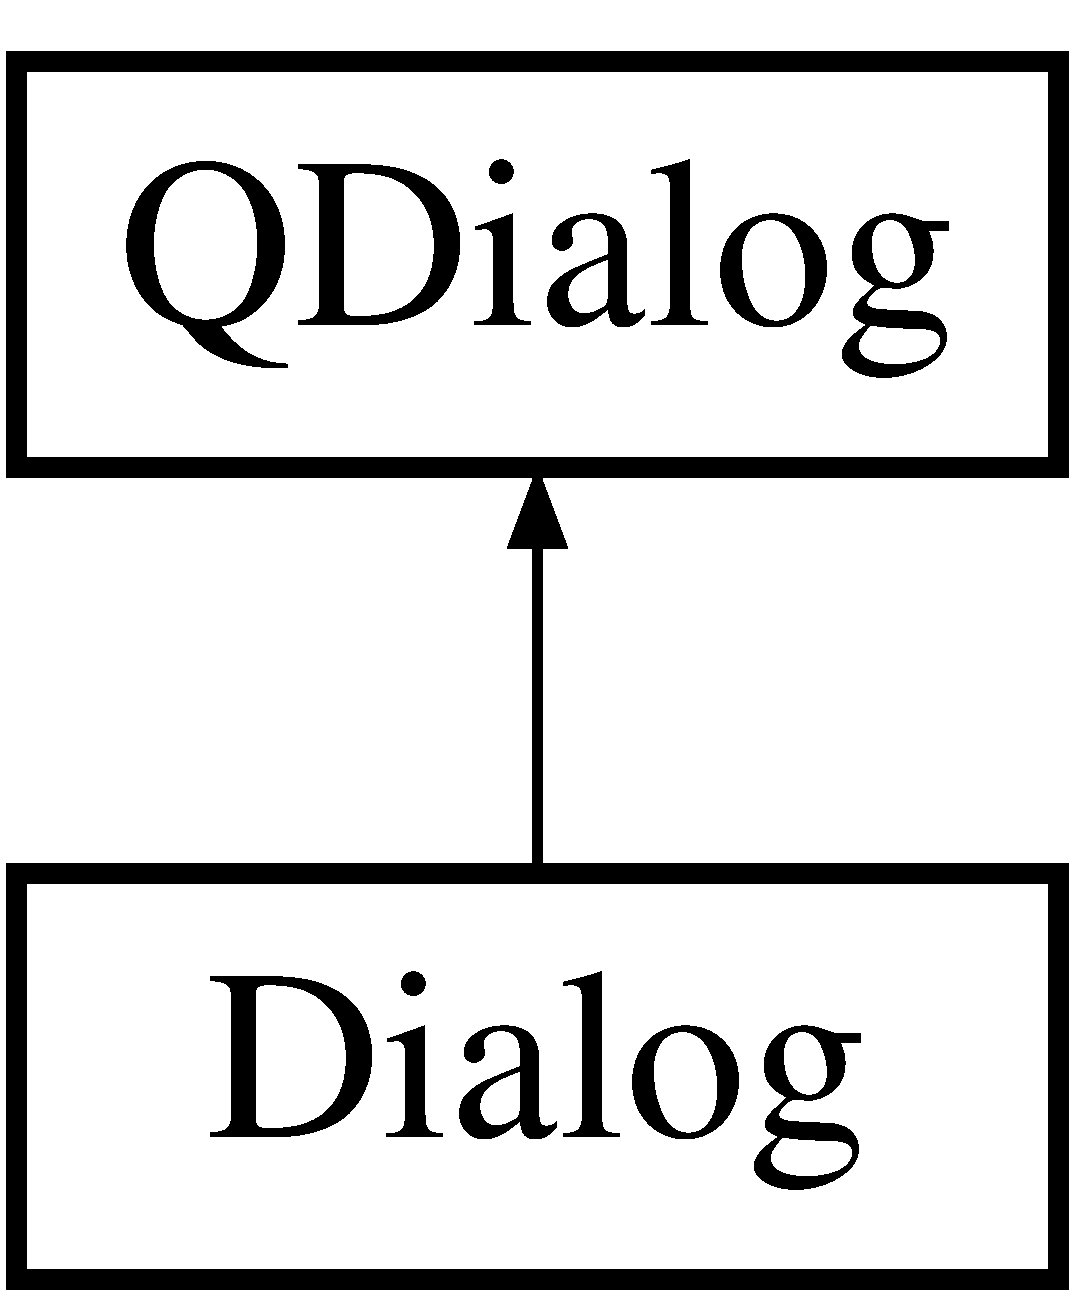
\includegraphics[height=2.000000cm]{class_dialog}
\end{center}
\end{figure}
\subsection*{Public Member Functions}
\begin{DoxyCompactItemize}
\item 
\hyperlink{class_dialog_acfa2063f9f962d394c6a645b6e7e08d8}{Dialog} (Q\+Widget $\ast$parent=0)
\begin{DoxyCompactList}\small\item\em Constructor of the \hyperlink{class_dialog}{Dialog}. \end{DoxyCompactList}\item 
\hyperlink{class_dialog_a2a1fe6ef28513eed13bfcd3a4da83ccb}{$\sim$\+Dialog} ()
\begin{DoxyCompactList}\small\item\em Default destructor of the \hyperlink{class_dialog}{Dialog}. \end{DoxyCompactList}\item 
Q\+Dialog\+Button\+Box $\ast$const \hyperlink{class_dialog_a378ce1b268dfbb518ea04bb5a7032a4e}{get\+Button} ()
\begin{DoxyCompactList}\small\item\em Const Accessor method wich provide the button in order to connect it. \end{DoxyCompactList}\item 
\hyperlink{structset_of_values}{set\+Of\+Values} const  \& \hyperlink{class_dialog_a530b0b5779a9bfd94e47c271baa1af62}{get\+Struct} ()
\begin{DoxyCompactList}\small\item\em Const Accessor method wich provide the structure. \end{DoxyCompactList}\end{DoxyCompactItemize}


\subsection{Detailed Description}
Set the structure and the links between objects when parameters of the line are entered. 

\subsection{Constructor \& Destructor Documentation}
\hypertarget{class_dialog_acfa2063f9f962d394c6a645b6e7e08d8}{}\label{class_dialog_acfa2063f9f962d394c6a645b6e7e08d8} 
\index{Dialog@{Dialog}!Dialog@{Dialog}}
\index{Dialog@{Dialog}!Dialog@{Dialog}}
\subsubsection{\texorpdfstring{Dialog()}{Dialog()}}
{\footnotesize\ttfamily Dialog\+::\+Dialog (\begin{DoxyParamCaption}\item[{Q\+Widget $\ast$}]{parent = {\ttfamily 0} }\end{DoxyParamCaption})\hspace{0.3cm}{\ttfamily [explicit]}}



Constructor of the \hyperlink{class_dialog}{Dialog}. 


\begin{DoxyParams}{Parameters}
{\em parent} & the global widget \\
\hline
\end{DoxyParams}
\hypertarget{class_dialog_a2a1fe6ef28513eed13bfcd3a4da83ccb}{}\label{class_dialog_a2a1fe6ef28513eed13bfcd3a4da83ccb} 
\index{Dialog@{Dialog}!````~Dialog@{$\sim$\+Dialog}}
\index{````~Dialog@{$\sim$\+Dialog}!Dialog@{Dialog}}
\subsubsection{\texorpdfstring{$\sim$\+Dialog()}{~Dialog()}}
{\footnotesize\ttfamily Dialog\+::$\sim$\+Dialog (\begin{DoxyParamCaption}{ }\end{DoxyParamCaption})}



Default destructor of the \hyperlink{class_dialog}{Dialog}. 



\subsection{Member Function Documentation}
\hypertarget{class_dialog_a378ce1b268dfbb518ea04bb5a7032a4e}{}\label{class_dialog_a378ce1b268dfbb518ea04bb5a7032a4e} 
\index{Dialog@{Dialog}!get\+Button@{get\+Button}}
\index{get\+Button@{get\+Button}!Dialog@{Dialog}}
\subsubsection{\texorpdfstring{get\+Button()}{getButton()}}
{\footnotesize\ttfamily Q\+Dialog\+Button\+Box $\ast$const Dialog\+::get\+Button (\begin{DoxyParamCaption}{ }\end{DoxyParamCaption})}



Const Accessor method wich provide the button in order to connect it. 

\begin{DoxyReturn}{Returns}
The button 
\end{DoxyReturn}
\hypertarget{class_dialog_a530b0b5779a9bfd94e47c271baa1af62}{}\label{class_dialog_a530b0b5779a9bfd94e47c271baa1af62} 
\index{Dialog@{Dialog}!get\+Struct@{get\+Struct}}
\index{get\+Struct@{get\+Struct}!Dialog@{Dialog}}
\subsubsection{\texorpdfstring{get\+Struct()}{getStruct()}}
{\footnotesize\ttfamily \hyperlink{structset_of_values}{set\+Of\+Values} const  \& Dialog\+::get\+Struct (\begin{DoxyParamCaption}{ }\end{DoxyParamCaption})}



Const Accessor method wich provide the structure. 

\begin{DoxyReturn}{Returns}
The structure which belong to the window 
\end{DoxyReturn}


The documentation for this class was generated from the following files\+:\begin{DoxyCompactItemize}
\item 
D\+:/\+Q\+T\+\_\+projets/\+Cube\+Menu/\hyperlink{dialog_8h}{dialog.\+h}\item 
D\+:/\+Q\+T\+\_\+projets/\+Cube\+Menu/\hyperlink{dialog_8cpp}{dialog.\+cpp}\end{DoxyCompactItemize}

\hypertarget{class_ui_1_1_dialog}{}\section{Ui\+:\+:Dialog Class Reference}
\label{class_ui_1_1_dialog}\index{Ui\+::\+Dialog@{Ui\+::\+Dialog}}


{\ttfamily \#include $<$ui\+\_\+dialog.\+h$>$}

Inheritance diagram for Ui\+:\+:Dialog\+:\begin{figure}[H]
\begin{center}
\leavevmode
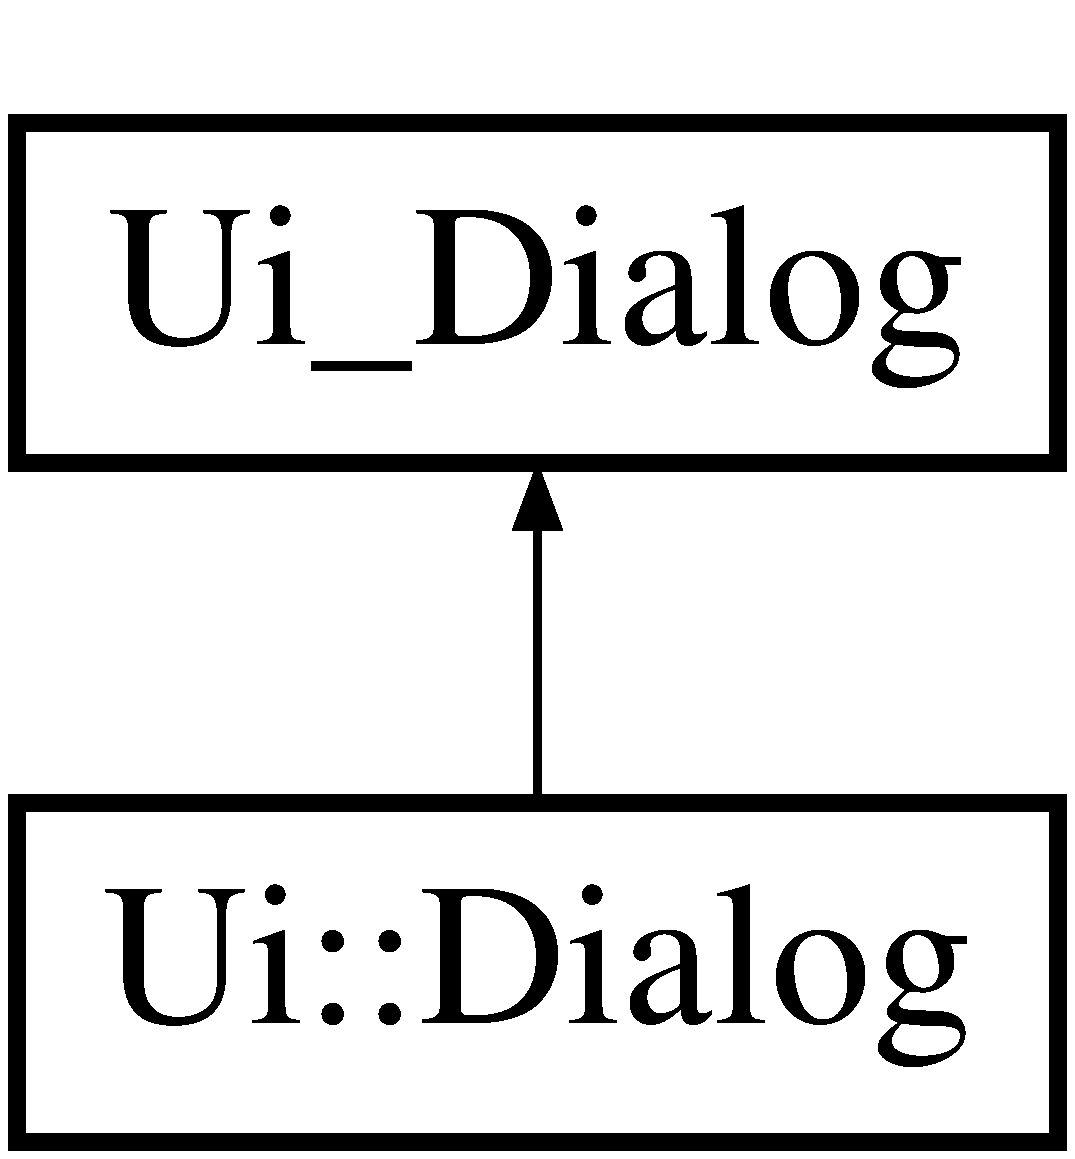
\includegraphics[height=2.000000cm]{class_ui_1_1_dialog}
\end{center}
\end{figure}
\subsection*{Additional Inherited Members}


The documentation for this class was generated from the following file\+:\begin{DoxyCompactItemize}
\item 
D\+:/\+Q\+T\+\_\+projets/\+Cube\+Menu/\hyperlink{ui__dialog_8h}{ui\+\_\+dialog.\+h}\end{DoxyCompactItemize}

\hypertarget{class_ui_1_1_dialog__view}{}\section{Ui\+:\+:Dialog\+\_\+view Class Reference}
\label{class_ui_1_1_dialog__view}\index{Ui\+::\+Dialog\+\_\+view@{Ui\+::\+Dialog\+\_\+view}}


{\ttfamily \#include $<$ui\+\_\+dialog\+\_\+view.\+h$>$}

Inheritance diagram for Ui\+:\+:Dialog\+\_\+view\+:\begin{figure}[H]
\begin{center}
\leavevmode
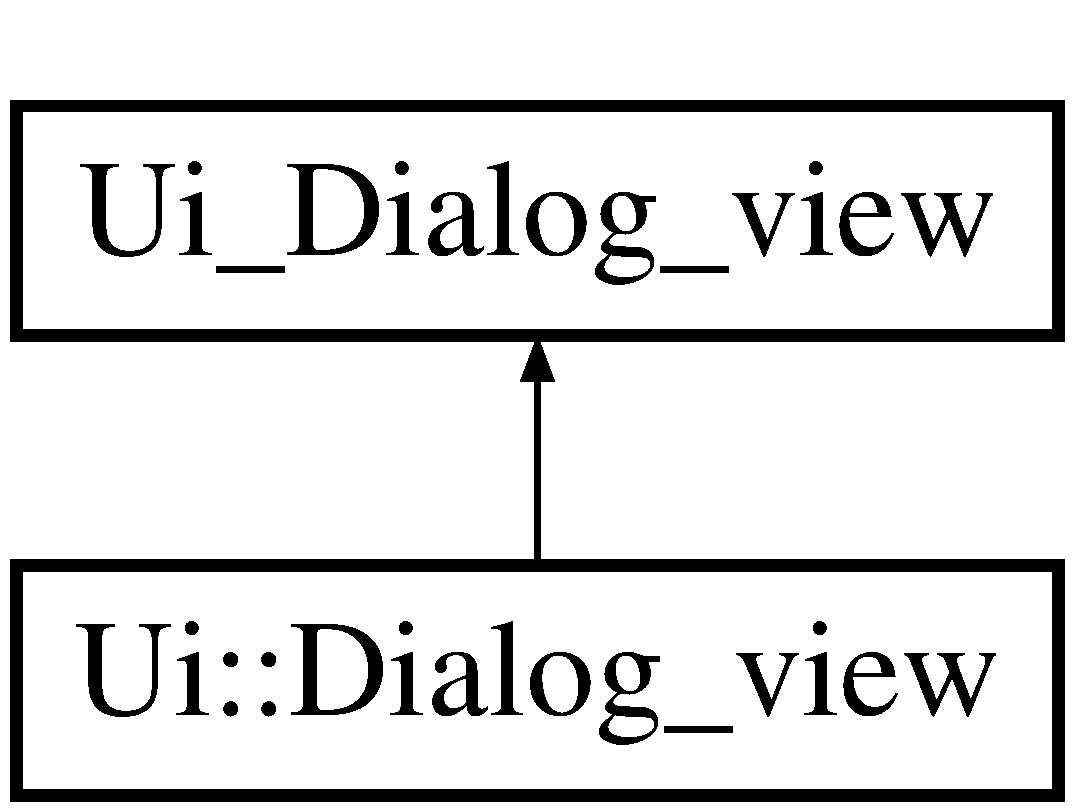
\includegraphics[height=2.000000cm]{class_ui_1_1_dialog__view}
\end{center}
\end{figure}
\subsection*{Additional Inherited Members}


The documentation for this class was generated from the following file\+:\begin{DoxyCompactItemize}
\item 
D\+:/\+Q\+T\+\_\+projets/\+Cube\+Menu/\hyperlink{ui__dialog__view_8h}{ui\+\_\+dialog\+\_\+view.\+h}\end{DoxyCompactItemize}

\hypertarget{class_dialog_eyes}{}\section{Dialog\+Eyes Class Reference}
\label{class_dialog_eyes}\index{Dialog\+Eyes@{Dialog\+Eyes}}


Set the structure and the links between objects when parameters of the view are entered.  




{\ttfamily \#include $<$dialogeyes.\+h$>$}

Inheritance diagram for Dialog\+Eyes\+:\begin{figure}[H]
\begin{center}
\leavevmode
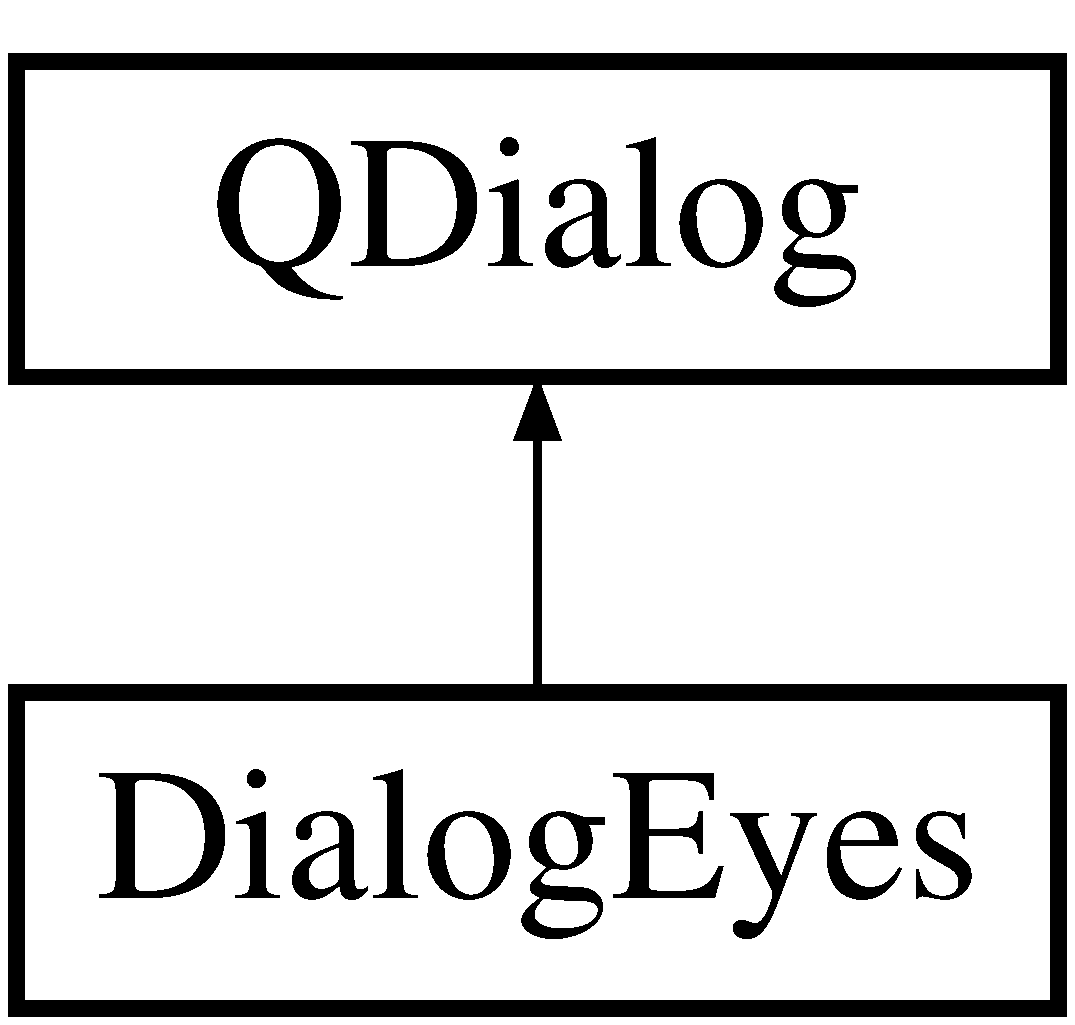
\includegraphics[height=2.000000cm]{class_dialog_eyes}
\end{center}
\end{figure}
\subsection*{Public Member Functions}
\begin{DoxyCompactItemize}
\item 
\hyperlink{class_dialog_eyes_a97beed52342196a6063d41f03dd63953}{Dialog\+Eyes} (Q\+Widget $\ast$parent=0)
\begin{DoxyCompactList}\small\item\em Constructor of the \hyperlink{class_dialog_eyes}{Dialog\+Eyes}. \end{DoxyCompactList}\item 
\hyperlink{class_dialog_eyes_a751e612833e5556f5c53dfc4875ef252}{$\sim$\+Dialog\+Eyes} ()
\begin{DoxyCompactList}\small\item\em Default destructor of the \hyperlink{class_dialog_eyes}{Dialog\+Eyes}. \end{DoxyCompactList}\item 
Q\+Dialog\+Button\+Box $\ast$const \hyperlink{class_dialog_eyes_a29267293c5a4b873aa59c7baafd65227}{get\+Button} ()
\begin{DoxyCompactList}\small\item\em Const Accessor method wich provide the button in order to connect it. \end{DoxyCompactList}\item 
\hyperlink{structset_of_view}{set\+Of\+View} const  \& \hyperlink{class_dialog_eyes_a71df236a91eafd03c9747ec3d245d017}{get\+Struct} ()
\begin{DoxyCompactList}\small\item\em Const Accessor method wich provide the structure. \end{DoxyCompactList}\end{DoxyCompactItemize}


\subsection{Detailed Description}
Set the structure and the links between objects when parameters of the view are entered. 

\subsection{Constructor \& Destructor Documentation}
\hypertarget{class_dialog_eyes_a97beed52342196a6063d41f03dd63953}{}\label{class_dialog_eyes_a97beed52342196a6063d41f03dd63953} 
\index{Dialog\+Eyes@{Dialog\+Eyes}!Dialog\+Eyes@{Dialog\+Eyes}}
\index{Dialog\+Eyes@{Dialog\+Eyes}!Dialog\+Eyes@{Dialog\+Eyes}}
\subsubsection{\texorpdfstring{Dialog\+Eyes()}{DialogEyes()}}
{\footnotesize\ttfamily Dialog\+Eyes\+::\+Dialog\+Eyes (\begin{DoxyParamCaption}\item[{Q\+Widget $\ast$}]{parent = {\ttfamily 0} }\end{DoxyParamCaption})\hspace{0.3cm}{\ttfamily [explicit]}}



Constructor of the \hyperlink{class_dialog_eyes}{Dialog\+Eyes}. 


\begin{DoxyParams}{Parameters}
{\em parent} & the global widget \\
\hline
\end{DoxyParams}
\hypertarget{class_dialog_eyes_a751e612833e5556f5c53dfc4875ef252}{}\label{class_dialog_eyes_a751e612833e5556f5c53dfc4875ef252} 
\index{Dialog\+Eyes@{Dialog\+Eyes}!````~Dialog\+Eyes@{$\sim$\+Dialog\+Eyes}}
\index{````~Dialog\+Eyes@{$\sim$\+Dialog\+Eyes}!Dialog\+Eyes@{Dialog\+Eyes}}
\subsubsection{\texorpdfstring{$\sim$\+Dialog\+Eyes()}{~DialogEyes()}}
{\footnotesize\ttfamily Dialog\+Eyes\+::$\sim$\+Dialog\+Eyes (\begin{DoxyParamCaption}{ }\end{DoxyParamCaption})}



Default destructor of the \hyperlink{class_dialog_eyes}{Dialog\+Eyes}. 



\subsection{Member Function Documentation}
\hypertarget{class_dialog_eyes_a29267293c5a4b873aa59c7baafd65227}{}\label{class_dialog_eyes_a29267293c5a4b873aa59c7baafd65227} 
\index{Dialog\+Eyes@{Dialog\+Eyes}!get\+Button@{get\+Button}}
\index{get\+Button@{get\+Button}!Dialog\+Eyes@{Dialog\+Eyes}}
\subsubsection{\texorpdfstring{get\+Button()}{getButton()}}
{\footnotesize\ttfamily Q\+Dialog\+Button\+Box $\ast$const Dialog\+Eyes\+::get\+Button (\begin{DoxyParamCaption}{ }\end{DoxyParamCaption})}



Const Accessor method wich provide the button in order to connect it. 

\begin{DoxyReturn}{Returns}
The button 
\end{DoxyReturn}
\hypertarget{class_dialog_eyes_a71df236a91eafd03c9747ec3d245d017}{}\label{class_dialog_eyes_a71df236a91eafd03c9747ec3d245d017} 
\index{Dialog\+Eyes@{Dialog\+Eyes}!get\+Struct@{get\+Struct}}
\index{get\+Struct@{get\+Struct}!Dialog\+Eyes@{Dialog\+Eyes}}
\subsubsection{\texorpdfstring{get\+Struct()}{getStruct()}}
{\footnotesize\ttfamily const \hyperlink{structset_of_view}{set\+Of\+View} \& Dialog\+Eyes\+::get\+Struct (\begin{DoxyParamCaption}{ }\end{DoxyParamCaption})}



Const Accessor method wich provide the structure. 

\begin{DoxyReturn}{Returns}
The structure which belong to the window 
\end{DoxyReturn}


The documentation for this class was generated from the following files\+:\begin{DoxyCompactItemize}
\item 
D\+:/\+Q\+T\+\_\+projets/\+Cube\+Menu/\hyperlink{dialogeyes_8h}{dialogeyes.\+h}\item 
D\+:/\+Q\+T\+\_\+projets/\+Cube\+Menu/\hyperlink{dialogeyes_8cpp}{dialogeyes.\+cpp}\end{DoxyCompactItemize}

\hypertarget{class_ui_1_1_dialog_eyes}{}\section{Ui\+:\+:Dialog\+Eyes Class Reference}
\label{class_ui_1_1_dialog_eyes}\index{Ui\+::\+Dialog\+Eyes@{Ui\+::\+Dialog\+Eyes}}


{\ttfamily \#include $<$ui\+\_\+dialogeyes.\+h$>$}

Inheritance diagram for Ui\+:\+:Dialog\+Eyes\+:\begin{figure}[H]
\begin{center}
\leavevmode
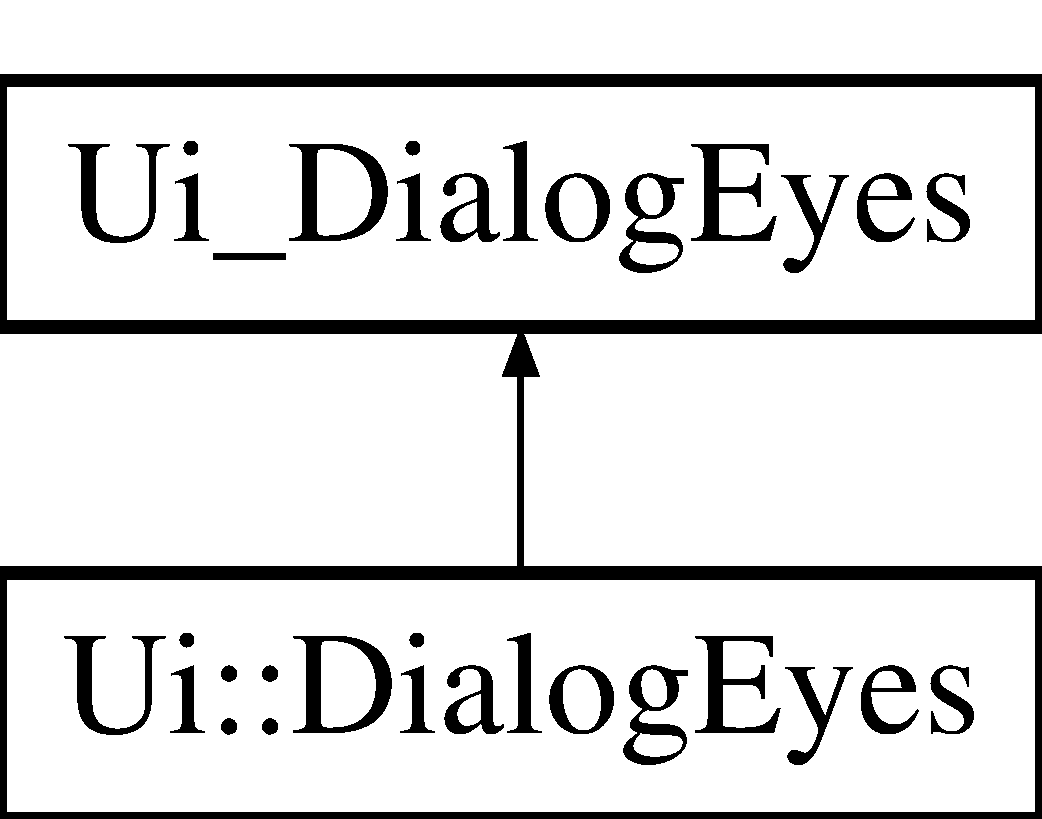
\includegraphics[height=2.000000cm]{class_ui_1_1_dialog_eyes}
\end{center}
\end{figure}
\subsection*{Additional Inherited Members}


The documentation for this class was generated from the following file\+:\begin{DoxyCompactItemize}
\item 
D\+:/\+Q\+T\+\_\+projets/\+Cube\+Menu/\hyperlink{ui__dialogeyes_8h}{ui\+\_\+dialogeyes.\+h}\end{DoxyCompactItemize}

\hypertarget{class_g_l_s_l_program}{}\section{G\+L\+S\+L\+Program Class Reference}
\label{class_g_l_s_l_program}\index{G\+L\+S\+L\+Program@{G\+L\+S\+L\+Program}}


{\ttfamily \#include $<$glslprogram.\+h$>$}

\subsection*{Public Member Functions}
\begin{DoxyCompactItemize}
\item 
\hyperlink{class_g_l_s_l_program_a9a93ab534634ee4abfda2f216008e553}{G\+L\+S\+L\+Program} ()
\begin{DoxyCompactList}\small\item\em Default constructor of \hyperlink{class_g_l_s_l_program}{G\+L\+S\+L\+Program}. \end{DoxyCompactList}\item 
bool \hyperlink{class_g_l_s_l_program_a31f24024046d5ed7646d0c53df4898dc}{compile\+Shader\+From\+File} (const char $\ast$file\+Name, \hyperlink{namespace_g_l_s_l_shader_a5da03bdfde28d414fcf090182b3b8177}{G\+L\+S\+L\+Shader\+::\+G\+L\+S\+L\+Shader\+Type} type)
\begin{DoxyCompactList}\small\item\em Read the shader source from a file and compile. \end{DoxyCompactList}\item 
bool \hyperlink{class_g_l_s_l_program_a428c7ce6d50b7100d06c621e6647dda8}{compile\+Shader\+From\+String} (const string \&source, \hyperlink{namespace_g_l_s_l_shader_a5da03bdfde28d414fcf090182b3b8177}{G\+L\+S\+L\+Shader\+::\+G\+L\+S\+L\+Shader\+Type} type)
\begin{DoxyCompactList}\small\item\em Compiles shader source code stored in a string. \end{DoxyCompactList}\item 
std\+::string \hyperlink{class_g_l_s_l_program_afc8f73c15d9696c49783b86a187123be}{load\+File\+To\+String} (const char $\ast$fname)
\begin{DoxyCompactList}\small\item\em Load the shader source code from the file into a string. \end{DoxyCompactList}\item 
void \hyperlink{class_g_l_s_l_program_afe85e8fe71e8b906f72ca3858531fa39}{load\+\_\+shader} (G\+Luint shaderobject, const char $\ast$shadersourcefilename)
\begin{DoxyCompactList}\small\item\em Load the shader code from a file. \end{DoxyCompactList}\item 
void \hyperlink{class_g_l_s_l_program_ae34d52138ce5780b39a6396e68b90349}{glcpp\+Shader\+Source} (G\+Luint shader, std\+::string const \&shader\+\_\+string)
\begin{DoxyCompactList}\small\item\em gl\+Shader\+Source sets the source code in shader to the source code in the array of strings specified by string. \end{DoxyCompactList}\item 
G\+Luint \hyperlink{class_g_l_s_l_program_ae4fe65254ed23ef5fba32dd4b7a3bee2}{create\+Shader} (G\+Lenum shader\+Type)
\begin{DoxyCompactList}\small\item\em gl\+Create\+Shader creates an empty shader object and returns a non-\/zero value by which it can be referenced. \end{DoxyCompactList}\item 
void \hyperlink{class_g_l_s_l_program_ae1ebde6b1ea8269f37064adb8e6d857f}{compile\+Shader} (G\+Luint shader)
\begin{DoxyCompactList}\small\item\em gl\+Compile\+Shader compiles the source code strings that have been stored in the shader object specified by shader. \end{DoxyCompactList}\item 
void \hyperlink{class_g_l_s_l_program_a4eebc77a6efe271bbf5eba25e8a27b66}{check\+Compile\+Status} (G\+Luint shader)
\begin{DoxyCompactList}\small\item\em Provides error log information for compilation of shader. \end{DoxyCompactList}\item 
void \hyperlink{class_g_l_s_l_program_a4b09d65133e3d9495315c2db2fb9295d}{attach\+Shader} (G\+Luint shader)
\begin{DoxyCompactList}\small\item\em Attaches the shader object specified by shader to the program object specified by handle. \end{DoxyCompactList}\item 
bool \hyperlink{class_g_l_s_l_program_a79c92c1c9a1a09c0a091cd52a8f602c6}{link} ()
\item 
void \hyperlink{class_g_l_s_l_program_a0ea2aeacb4361b37f145246430134bb6}{use} ()
\item 
bool \hyperlink{class_g_l_s_l_program_a07aaaf69f5837deb59a7551dc323f667}{create\+Object} ()
\item 
string \hyperlink{class_g_l_s_l_program_ac03cbf803fbcc60d3ff4b3b6d4ecbaa6}{log} ()
\item 
G\+Luint \hyperlink{class_g_l_s_l_program_a37f5a6e85135bc51ed4a94712bacde76}{get\+Handle} ()
\item 
bool \hyperlink{class_g_l_s_l_program_ad0d1efa38db415e35d9a329a93828815}{is\+Linked} ()
\item 
void \hyperlink{class_g_l_s_l_program_a54589ae245f6fac51f79a6617c91240b}{bind\+Attrib\+Location} (G\+Luint location, const char $\ast$name)
\begin{DoxyCompactList}\small\item\em associates a user-\/defined attribute variable in the program object specified by handle with a generic vertex attribute index. \end{DoxyCompactList}\item 
void \hyperlink{class_g_l_s_l_program_a44270f942de121ef2493e26f1226a902}{bind\+Frag\+Data\+Location} (G\+Luint location, const char $\ast$name)
\begin{DoxyCompactList}\small\item\em bind a user-\/defined varying out variable specified by name to a fragment shader color number specified by location \end{DoxyCompactList}\item 
void \hyperlink{class_g_l_s_l_program_a85e4c896c2a8524cb4574a064a2dfb0c}{set\+Uniform} (const char $\ast$name, float x, float y, float z)
\begin{DoxyCompactList}\small\item\em x,y,z are the new values to be used for the specified uniform variable \end{DoxyCompactList}\item 
void \hyperlink{class_g_l_s_l_program_a8784d794a6dbe97903d85bd0135a61c8}{set\+Uniform} (const char $\ast$name, const vec3 \&v)
\begin{DoxyCompactList}\small\item\em v.\+x,v.\+y,v.\+z are the new values to be used for the specified uniform variable \end{DoxyCompactList}\item 
void \hyperlink{class_g_l_s_l_program_aadf3691c119baac516735b0d01b85f7e}{set\+Uniform} (const char $\ast$name, const vec4 \&v)
\begin{DoxyCompactList}\small\item\em v.\+x,v.\+y,v.\+z, v.\+w are the new values to be used for the specified uniform variable \end{DoxyCompactList}\item 
void \hyperlink{class_g_l_s_l_program_aae087de52f91a47ac23c9f6ebf369bc3}{set\+Uniform} (const char $\ast$name, float val)
\begin{DoxyCompactList}\small\item\em val is the new value for the uniform variable \end{DoxyCompactList}\item 
void \hyperlink{class_g_l_s_l_program_a437782e359f10918044f1bbad0a98148}{set\+Uniform} (const char $\ast$name, int val)
\begin{DoxyCompactList}\small\item\em val is the new value for the uniform variable \end{DoxyCompactList}\item 
void \hyperlink{class_g_l_s_l_program_acfab16fafb4617f0625f170b39716eb8}{set\+Uniform} (const char $\ast$name, bool val)
\begin{DoxyCompactList}\small\item\em val is the new value for the uniform variable \end{DoxyCompactList}\item 
void \hyperlink{class_g_l_s_l_program_a44a7ace14e6c82311526e47264957fa9}{set\+Uniform} (const char $\ast$name, const mat4 \&m)
\begin{DoxyCompactList}\small\item\em The commands gl\+Uniform\+Matrix\{2$\vert$3$\vert$4\}fv are used to modify a matrix or an array of matrices. The numbers in the command name are interpreted as the dimensionality of the matrix. \end{DoxyCompactList}\item 
void \hyperlink{class_g_l_s_l_program_a69bd967b17f6b06e9fd4772b25e86396}{set\+Uniform} (const char $\ast$name, const mat3 \&m)
\begin{DoxyCompactList}\small\item\em The commands gl\+Uniform\+Matrix\{2$\vert$3$\vert$4\}fv are used to modify a matrix or an array of matrices. The numbers in the command name are interpreted as the dimensionality of the matrix. \end{DoxyCompactList}\item 
void \hyperlink{class_g_l_s_l_program_a75e11d36a5b634c58a84caa96c9c38e4}{print\+Active\+Uniforms} ()
\begin{DoxyCompactList}\small\item\em Prints all the active uniform variables. \end{DoxyCompactList}\item 
void \hyperlink{class_g_l_s_l_program_aab7c8bc0e5d0b75a9eb0c60de3cda5b5}{print\+Active\+Attribs} ()
\begin{DoxyCompactList}\small\item\em Prints all the active attribute variables. \end{DoxyCompactList}\end{DoxyCompactItemize}


\subsection{Constructor \& Destructor Documentation}
\hypertarget{class_g_l_s_l_program_a9a93ab534634ee4abfda2f216008e553}{}\label{class_g_l_s_l_program_a9a93ab534634ee4abfda2f216008e553} 
\index{G\+L\+S\+L\+Program@{G\+L\+S\+L\+Program}!G\+L\+S\+L\+Program@{G\+L\+S\+L\+Program}}
\index{G\+L\+S\+L\+Program@{G\+L\+S\+L\+Program}!G\+L\+S\+L\+Program@{G\+L\+S\+L\+Program}}
\subsubsection{\texorpdfstring{G\+L\+S\+L\+Program()}{GLSLProgram()}}
{\footnotesize\ttfamily G\+L\+S\+L\+Program\+::\+G\+L\+S\+L\+Program (\begin{DoxyParamCaption}{ }\end{DoxyParamCaption})}



Default constructor of \hyperlink{class_g_l_s_l_program}{G\+L\+S\+L\+Program}. 



\subsection{Member Function Documentation}
\hypertarget{class_g_l_s_l_program_a4b09d65133e3d9495315c2db2fb9295d}{}\label{class_g_l_s_l_program_a4b09d65133e3d9495315c2db2fb9295d} 
\index{G\+L\+S\+L\+Program@{G\+L\+S\+L\+Program}!attach\+Shader@{attach\+Shader}}
\index{attach\+Shader@{attach\+Shader}!G\+L\+S\+L\+Program@{G\+L\+S\+L\+Program}}
\subsubsection{\texorpdfstring{attach\+Shader()}{attachShader()}}
{\footnotesize\ttfamily void G\+L\+S\+L\+Program\+::attach\+Shader (\begin{DoxyParamCaption}\item[{G\+Luint}]{shader }\end{DoxyParamCaption})}



Attaches the shader object specified by shader to the program object specified by handle. 


\begin{DoxyParams}{Parameters}
{\em shader} & shader \\
\hline
\end{DoxyParams}
\hypertarget{class_g_l_s_l_program_a54589ae245f6fac51f79a6617c91240b}{}\label{class_g_l_s_l_program_a54589ae245f6fac51f79a6617c91240b} 
\index{G\+L\+S\+L\+Program@{G\+L\+S\+L\+Program}!bind\+Attrib\+Location@{bind\+Attrib\+Location}}
\index{bind\+Attrib\+Location@{bind\+Attrib\+Location}!G\+L\+S\+L\+Program@{G\+L\+S\+L\+Program}}
\subsubsection{\texorpdfstring{bind\+Attrib\+Location()}{bindAttribLocation()}}
{\footnotesize\ttfamily void G\+L\+S\+L\+Program\+::bind\+Attrib\+Location (\begin{DoxyParamCaption}\item[{G\+Luint}]{location,  }\item[{const char $\ast$}]{name }\end{DoxyParamCaption})}



associates a user-\/defined attribute variable in the program object specified by handle with a generic vertex attribute index. 


\begin{DoxyParams}{Parameters}
{\em location} & location of the G\+Luint \\
\hline
{\em name} & name \\
\hline
\end{DoxyParams}
\hypertarget{class_g_l_s_l_program_a44270f942de121ef2493e26f1226a902}{}\label{class_g_l_s_l_program_a44270f942de121ef2493e26f1226a902} 
\index{G\+L\+S\+L\+Program@{G\+L\+S\+L\+Program}!bind\+Frag\+Data\+Location@{bind\+Frag\+Data\+Location}}
\index{bind\+Frag\+Data\+Location@{bind\+Frag\+Data\+Location}!G\+L\+S\+L\+Program@{G\+L\+S\+L\+Program}}
\subsubsection{\texorpdfstring{bind\+Frag\+Data\+Location()}{bindFragDataLocation()}}
{\footnotesize\ttfamily void G\+L\+S\+L\+Program\+::bind\+Frag\+Data\+Location (\begin{DoxyParamCaption}\item[{G\+Luint}]{location,  }\item[{const char $\ast$}]{name }\end{DoxyParamCaption})}



bind a user-\/defined varying out variable specified by name to a fragment shader color number specified by location 


\begin{DoxyParams}{Parameters}
{\em location} & location of the G\+Luint \\
\hline
{\em name} & name \\
\hline
\end{DoxyParams}
\hypertarget{class_g_l_s_l_program_a4eebc77a6efe271bbf5eba25e8a27b66}{}\label{class_g_l_s_l_program_a4eebc77a6efe271bbf5eba25e8a27b66} 
\index{G\+L\+S\+L\+Program@{G\+L\+S\+L\+Program}!check\+Compile\+Status@{check\+Compile\+Status}}
\index{check\+Compile\+Status@{check\+Compile\+Status}!G\+L\+S\+L\+Program@{G\+L\+S\+L\+Program}}
\subsubsection{\texorpdfstring{check\+Compile\+Status()}{checkCompileStatus()}}
{\footnotesize\ttfamily void G\+L\+S\+L\+Program\+::check\+Compile\+Status (\begin{DoxyParamCaption}\item[{G\+Luint}]{shader }\end{DoxyParamCaption})}



Provides error log information for compilation of shader. 


\begin{DoxyParams}{Parameters}
{\em shader} & shader \\
\hline
\end{DoxyParams}
\hypertarget{class_g_l_s_l_program_ae1ebde6b1ea8269f37064adb8e6d857f}{}\label{class_g_l_s_l_program_ae1ebde6b1ea8269f37064adb8e6d857f} 
\index{G\+L\+S\+L\+Program@{G\+L\+S\+L\+Program}!compile\+Shader@{compile\+Shader}}
\index{compile\+Shader@{compile\+Shader}!G\+L\+S\+L\+Program@{G\+L\+S\+L\+Program}}
\subsubsection{\texorpdfstring{compile\+Shader()}{compileShader()}}
{\footnotesize\ttfamily void G\+L\+S\+L\+Program\+::compile\+Shader (\begin{DoxyParamCaption}\item[{G\+Luint}]{shader }\end{DoxyParamCaption})}



gl\+Compile\+Shader compiles the source code strings that have been stored in the shader object specified by shader. 


\begin{DoxyParams}{Parameters}
{\em shader} & shader \\
\hline
\end{DoxyParams}
\hypertarget{class_g_l_s_l_program_a31f24024046d5ed7646d0c53df4898dc}{}\label{class_g_l_s_l_program_a31f24024046d5ed7646d0c53df4898dc} 
\index{G\+L\+S\+L\+Program@{G\+L\+S\+L\+Program}!compile\+Shader\+From\+File@{compile\+Shader\+From\+File}}
\index{compile\+Shader\+From\+File@{compile\+Shader\+From\+File}!G\+L\+S\+L\+Program@{G\+L\+S\+L\+Program}}
\subsubsection{\texorpdfstring{compile\+Shader\+From\+File()}{compileShaderFromFile()}}
{\footnotesize\ttfamily bool G\+L\+S\+L\+Program\+::compile\+Shader\+From\+File (\begin{DoxyParamCaption}\item[{const char $\ast$}]{file\+Name,  }\item[{\hyperlink{namespace_g_l_s_l_shader_a5da03bdfde28d414fcf090182b3b8177}{G\+L\+S\+L\+Shader\+::\+G\+L\+S\+L\+Shader\+Type}}]{type }\end{DoxyParamCaption})}



Read the shader source from a file and compile. 


\begin{DoxyParams}{Parameters}
{\em file\+Name} & \+: name of the file \\
\hline
{\em type} & \+: type of shader \\
\hline
\end{DoxyParams}
\hypertarget{class_g_l_s_l_program_a428c7ce6d50b7100d06c621e6647dda8}{}\label{class_g_l_s_l_program_a428c7ce6d50b7100d06c621e6647dda8} 
\index{G\+L\+S\+L\+Program@{G\+L\+S\+L\+Program}!compile\+Shader\+From\+String@{compile\+Shader\+From\+String}}
\index{compile\+Shader\+From\+String@{compile\+Shader\+From\+String}!G\+L\+S\+L\+Program@{G\+L\+S\+L\+Program}}
\subsubsection{\texorpdfstring{compile\+Shader\+From\+String()}{compileShaderFromString()}}
{\footnotesize\ttfamily bool G\+L\+S\+L\+Program\+::compile\+Shader\+From\+String (\begin{DoxyParamCaption}\item[{const string \&}]{source,  }\item[{\hyperlink{namespace_g_l_s_l_shader_a5da03bdfde28d414fcf090182b3b8177}{G\+L\+S\+L\+Shader\+::\+G\+L\+S\+L\+Shader\+Type}}]{type }\end{DoxyParamCaption})}



Compiles shader source code stored in a string. 


\begin{DoxyParams}{Parameters}
{\em source} & \+: source of the shader \\
\hline
{\em type} & \+: type of shader \\
\hline
\end{DoxyParams}
\hypertarget{class_g_l_s_l_program_a07aaaf69f5837deb59a7551dc323f667}{}\label{class_g_l_s_l_program_a07aaaf69f5837deb59a7551dc323f667} 
\index{G\+L\+S\+L\+Program@{G\+L\+S\+L\+Program}!create\+Object@{create\+Object}}
\index{create\+Object@{create\+Object}!G\+L\+S\+L\+Program@{G\+L\+S\+L\+Program}}
\subsubsection{\texorpdfstring{create\+Object()}{createObject()}}
{\footnotesize\ttfamily bool G\+L\+S\+L\+Program\+::create\+Object (\begin{DoxyParamCaption}{ }\end{DoxyParamCaption})}

Creates an empty program object and returns a non-\/zero value by which it can be referenced. \hypertarget{class_g_l_s_l_program_ae4fe65254ed23ef5fba32dd4b7a3bee2}{}\label{class_g_l_s_l_program_ae4fe65254ed23ef5fba32dd4b7a3bee2} 
\index{G\+L\+S\+L\+Program@{G\+L\+S\+L\+Program}!create\+Shader@{create\+Shader}}
\index{create\+Shader@{create\+Shader}!G\+L\+S\+L\+Program@{G\+L\+S\+L\+Program}}
\subsubsection{\texorpdfstring{create\+Shader()}{createShader()}}
{\footnotesize\ttfamily G\+Luint G\+L\+S\+L\+Program\+::create\+Shader (\begin{DoxyParamCaption}\item[{G\+Lenum}]{shader\+Type }\end{DoxyParamCaption})}



gl\+Create\+Shader creates an empty shader object and returns a non-\/zero value by which it can be referenced. 


\begin{DoxyParams}{Parameters}
{\em shader\+Type} & type of the shader \\
\hline
\end{DoxyParams}
\hypertarget{class_g_l_s_l_program_a37f5a6e85135bc51ed4a94712bacde76}{}\label{class_g_l_s_l_program_a37f5a6e85135bc51ed4a94712bacde76} 
\index{G\+L\+S\+L\+Program@{G\+L\+S\+L\+Program}!get\+Handle@{get\+Handle}}
\index{get\+Handle@{get\+Handle}!G\+L\+S\+L\+Program@{G\+L\+S\+L\+Program}}
\subsubsection{\texorpdfstring{get\+Handle()}{getHandle()}}
{\footnotesize\ttfamily G\+Luint G\+L\+S\+L\+Program\+::get\+Handle (\begin{DoxyParamCaption}{ }\end{DoxyParamCaption})}

Return the program object handle \hypertarget{class_g_l_s_l_program_ae34d52138ce5780b39a6396e68b90349}{}\label{class_g_l_s_l_program_ae34d52138ce5780b39a6396e68b90349} 
\index{G\+L\+S\+L\+Program@{G\+L\+S\+L\+Program}!glcpp\+Shader\+Source@{glcpp\+Shader\+Source}}
\index{glcpp\+Shader\+Source@{glcpp\+Shader\+Source}!G\+L\+S\+L\+Program@{G\+L\+S\+L\+Program}}
\subsubsection{\texorpdfstring{glcpp\+Shader\+Source()}{glcppShaderSource()}}
{\footnotesize\ttfamily void G\+L\+S\+L\+Program\+::glcpp\+Shader\+Source (\begin{DoxyParamCaption}\item[{G\+Luint}]{shader,  }\item[{std\+::string const \&}]{shader\+\_\+string }\end{DoxyParamCaption})}



gl\+Shader\+Source sets the source code in shader to the source code in the array of strings specified by string. 


\begin{DoxyParams}{Parameters}
{\em shader} & \+: shader \\
\hline
{\em shader\+\_\+string} & \+: name of the file of the shader (string) \\
\hline
\end{DoxyParams}
\hypertarget{class_g_l_s_l_program_ad0d1efa38db415e35d9a329a93828815}{}\label{class_g_l_s_l_program_ad0d1efa38db415e35d9a329a93828815} 
\index{G\+L\+S\+L\+Program@{G\+L\+S\+L\+Program}!is\+Linked@{is\+Linked}}
\index{is\+Linked@{is\+Linked}!G\+L\+S\+L\+Program@{G\+L\+S\+L\+Program}}
\subsubsection{\texorpdfstring{is\+Linked()}{isLinked()}}
{\footnotesize\ttfamily bool G\+L\+S\+L\+Program\+::is\+Linked (\begin{DoxyParamCaption}{ }\end{DoxyParamCaption})}

Returns the link status \hypertarget{class_g_l_s_l_program_a79c92c1c9a1a09c0a091cd52a8f602c6}{}\label{class_g_l_s_l_program_a79c92c1c9a1a09c0a091cd52a8f602c6} 
\index{G\+L\+S\+L\+Program@{G\+L\+S\+L\+Program}!link@{link}}
\index{link@{link}!G\+L\+S\+L\+Program@{G\+L\+S\+L\+Program}}
\subsubsection{\texorpdfstring{link()}{link()}}
{\footnotesize\ttfamily bool G\+L\+S\+L\+Program\+::link (\begin{DoxyParamCaption}{ }\end{DoxyParamCaption})}

Links the program object specified by handle. \hypertarget{class_g_l_s_l_program_afe85e8fe71e8b906f72ca3858531fa39}{}\label{class_g_l_s_l_program_afe85e8fe71e8b906f72ca3858531fa39} 
\index{G\+L\+S\+L\+Program@{G\+L\+S\+L\+Program}!load\+\_\+shader@{load\+\_\+shader}}
\index{load\+\_\+shader@{load\+\_\+shader}!G\+L\+S\+L\+Program@{G\+L\+S\+L\+Program}}
\subsubsection{\texorpdfstring{load\+\_\+shader()}{load\_shader()}}
{\footnotesize\ttfamily void G\+L\+S\+L\+Program\+::load\+\_\+shader (\begin{DoxyParamCaption}\item[{G\+Luint}]{shaderobject,  }\item[{const char $\ast$}]{shadersourcefilename }\end{DoxyParamCaption})}



Load the shader code from a file. 


\begin{DoxyParams}{Parameters}
{\em shaderobject} & \+: shader object \\
\hline
{\em shadersourcefilename} & \+: name of the file of the shader \\
\hline
\end{DoxyParams}
\hypertarget{class_g_l_s_l_program_afc8f73c15d9696c49783b86a187123be}{}\label{class_g_l_s_l_program_afc8f73c15d9696c49783b86a187123be} 
\index{G\+L\+S\+L\+Program@{G\+L\+S\+L\+Program}!load\+File\+To\+String@{load\+File\+To\+String}}
\index{load\+File\+To\+String@{load\+File\+To\+String}!G\+L\+S\+L\+Program@{G\+L\+S\+L\+Program}}
\subsubsection{\texorpdfstring{load\+File\+To\+String()}{loadFileToString()}}
{\footnotesize\ttfamily std\+::string G\+L\+S\+L\+Program\+::load\+File\+To\+String (\begin{DoxyParamCaption}\item[{const char $\ast$}]{fname }\end{DoxyParamCaption})}



Load the shader source code from the file into a string. 


\begin{DoxyParams}{Parameters}
{\em fname} & \+: name of the file \\
\hline
\end{DoxyParams}
\hypertarget{class_g_l_s_l_program_ac03cbf803fbcc60d3ff4b3b6d4ecbaa6}{}\label{class_g_l_s_l_program_ac03cbf803fbcc60d3ff4b3b6d4ecbaa6} 
\index{G\+L\+S\+L\+Program@{G\+L\+S\+L\+Program}!log@{log}}
\index{log@{log}!G\+L\+S\+L\+Program@{G\+L\+S\+L\+Program}}
\subsubsection{\texorpdfstring{log()}{log()}}
{\footnotesize\ttfamily string G\+L\+S\+L\+Program\+::log (\begin{DoxyParamCaption}{ }\end{DoxyParamCaption})}

Returns the log\+String \hypertarget{class_g_l_s_l_program_aab7c8bc0e5d0b75a9eb0c60de3cda5b5}{}\label{class_g_l_s_l_program_aab7c8bc0e5d0b75a9eb0c60de3cda5b5} 
\index{G\+L\+S\+L\+Program@{G\+L\+S\+L\+Program}!print\+Active\+Attribs@{print\+Active\+Attribs}}
\index{print\+Active\+Attribs@{print\+Active\+Attribs}!G\+L\+S\+L\+Program@{G\+L\+S\+L\+Program}}
\subsubsection{\texorpdfstring{print\+Active\+Attribs()}{printActiveAttribs()}}
{\footnotesize\ttfamily void G\+L\+S\+L\+Program\+::print\+Active\+Attribs (\begin{DoxyParamCaption}{ }\end{DoxyParamCaption})}



Prints all the active attribute variables. 

\hypertarget{class_g_l_s_l_program_a75e11d36a5b634c58a84caa96c9c38e4}{}\label{class_g_l_s_l_program_a75e11d36a5b634c58a84caa96c9c38e4} 
\index{G\+L\+S\+L\+Program@{G\+L\+S\+L\+Program}!print\+Active\+Uniforms@{print\+Active\+Uniforms}}
\index{print\+Active\+Uniforms@{print\+Active\+Uniforms}!G\+L\+S\+L\+Program@{G\+L\+S\+L\+Program}}
\subsubsection{\texorpdfstring{print\+Active\+Uniforms()}{printActiveUniforms()}}
{\footnotesize\ttfamily void G\+L\+S\+L\+Program\+::print\+Active\+Uniforms (\begin{DoxyParamCaption}{ }\end{DoxyParamCaption})}



Prints all the active uniform variables. 

\hypertarget{class_g_l_s_l_program_a85e4c896c2a8524cb4574a064a2dfb0c}{}\label{class_g_l_s_l_program_a85e4c896c2a8524cb4574a064a2dfb0c} 
\index{G\+L\+S\+L\+Program@{G\+L\+S\+L\+Program}!set\+Uniform@{set\+Uniform}}
\index{set\+Uniform@{set\+Uniform}!G\+L\+S\+L\+Program@{G\+L\+S\+L\+Program}}
\subsubsection{\texorpdfstring{set\+Uniform()}{setUniform()}\hspace{0.1cm}{\footnotesize\ttfamily [1/8]}}
{\footnotesize\ttfamily void G\+L\+S\+L\+Program\+::set\+Uniform (\begin{DoxyParamCaption}\item[{const char $\ast$}]{name,  }\item[{float}]{x,  }\item[{float}]{y,  }\item[{float}]{z }\end{DoxyParamCaption})}



x,y,z are the new values to be used for the specified uniform variable 


\begin{DoxyParams}{Parameters}
{\em name} & name \\
\hline
{\em x} & coordinate x \\
\hline
{\em y} & coordinate y \\
\hline
{\em z} & coordinate z \\
\hline
\end{DoxyParams}
\hypertarget{class_g_l_s_l_program_a8784d794a6dbe97903d85bd0135a61c8}{}\label{class_g_l_s_l_program_a8784d794a6dbe97903d85bd0135a61c8} 
\index{G\+L\+S\+L\+Program@{G\+L\+S\+L\+Program}!set\+Uniform@{set\+Uniform}}
\index{set\+Uniform@{set\+Uniform}!G\+L\+S\+L\+Program@{G\+L\+S\+L\+Program}}
\subsubsection{\texorpdfstring{set\+Uniform()}{setUniform()}\hspace{0.1cm}{\footnotesize\ttfamily [2/8]}}
{\footnotesize\ttfamily void G\+L\+S\+L\+Program\+::set\+Uniform (\begin{DoxyParamCaption}\item[{const char $\ast$}]{name,  }\item[{const vec3 \&}]{v }\end{DoxyParamCaption})}



v.\+x,v.\+y,v.\+z are the new values to be used for the specified uniform variable 


\begin{DoxyParams}{Parameters}
{\em name} & name \\
\hline
{\em v} & vector of values \\
\hline
\end{DoxyParams}
\hypertarget{class_g_l_s_l_program_aadf3691c119baac516735b0d01b85f7e}{}\label{class_g_l_s_l_program_aadf3691c119baac516735b0d01b85f7e} 
\index{G\+L\+S\+L\+Program@{G\+L\+S\+L\+Program}!set\+Uniform@{set\+Uniform}}
\index{set\+Uniform@{set\+Uniform}!G\+L\+S\+L\+Program@{G\+L\+S\+L\+Program}}
\subsubsection{\texorpdfstring{set\+Uniform()}{setUniform()}\hspace{0.1cm}{\footnotesize\ttfamily [3/8]}}
{\footnotesize\ttfamily void G\+L\+S\+L\+Program\+::set\+Uniform (\begin{DoxyParamCaption}\item[{const char $\ast$}]{name,  }\item[{const vec4 \&}]{v }\end{DoxyParamCaption})}



v.\+x,v.\+y,v.\+z, v.\+w are the new values to be used for the specified uniform variable 


\begin{DoxyParams}{Parameters}
{\em name} & name \\
\hline
{\em v} & vector of values \\
\hline
\end{DoxyParams}
\hypertarget{class_g_l_s_l_program_aae087de52f91a47ac23c9f6ebf369bc3}{}\label{class_g_l_s_l_program_aae087de52f91a47ac23c9f6ebf369bc3} 
\index{G\+L\+S\+L\+Program@{G\+L\+S\+L\+Program}!set\+Uniform@{set\+Uniform}}
\index{set\+Uniform@{set\+Uniform}!G\+L\+S\+L\+Program@{G\+L\+S\+L\+Program}}
\subsubsection{\texorpdfstring{set\+Uniform()}{setUniform()}\hspace{0.1cm}{\footnotesize\ttfamily [4/8]}}
{\footnotesize\ttfamily void G\+L\+S\+L\+Program\+::set\+Uniform (\begin{DoxyParamCaption}\item[{const char $\ast$}]{name,  }\item[{float}]{val }\end{DoxyParamCaption})}



val is the new value for the uniform variable 


\begin{DoxyParams}{Parameters}
{\em name} & name \\
\hline
{\em val} & value of the uniform variable \\
\hline
\end{DoxyParams}
\hypertarget{class_g_l_s_l_program_a437782e359f10918044f1bbad0a98148}{}\label{class_g_l_s_l_program_a437782e359f10918044f1bbad0a98148} 
\index{G\+L\+S\+L\+Program@{G\+L\+S\+L\+Program}!set\+Uniform@{set\+Uniform}}
\index{set\+Uniform@{set\+Uniform}!G\+L\+S\+L\+Program@{G\+L\+S\+L\+Program}}
\subsubsection{\texorpdfstring{set\+Uniform()}{setUniform()}\hspace{0.1cm}{\footnotesize\ttfamily [5/8]}}
{\footnotesize\ttfamily void G\+L\+S\+L\+Program\+::set\+Uniform (\begin{DoxyParamCaption}\item[{const char $\ast$}]{name,  }\item[{int}]{val }\end{DoxyParamCaption})}



val is the new value for the uniform variable 


\begin{DoxyParams}{Parameters}
{\em name} & name \\
\hline
{\em val} & value of the uniform variable \\
\hline
\end{DoxyParams}
\hypertarget{class_g_l_s_l_program_acfab16fafb4617f0625f170b39716eb8}{}\label{class_g_l_s_l_program_acfab16fafb4617f0625f170b39716eb8} 
\index{G\+L\+S\+L\+Program@{G\+L\+S\+L\+Program}!set\+Uniform@{set\+Uniform}}
\index{set\+Uniform@{set\+Uniform}!G\+L\+S\+L\+Program@{G\+L\+S\+L\+Program}}
\subsubsection{\texorpdfstring{set\+Uniform()}{setUniform()}\hspace{0.1cm}{\footnotesize\ttfamily [6/8]}}
{\footnotesize\ttfamily void G\+L\+S\+L\+Program\+::set\+Uniform (\begin{DoxyParamCaption}\item[{const char $\ast$}]{name,  }\item[{bool}]{val }\end{DoxyParamCaption})}



val is the new value for the uniform variable 


\begin{DoxyParams}{Parameters}
{\em name} & name \\
\hline
{\em val} & value of the uniform variable \\
\hline
\end{DoxyParams}
\hypertarget{class_g_l_s_l_program_a44a7ace14e6c82311526e47264957fa9}{}\label{class_g_l_s_l_program_a44a7ace14e6c82311526e47264957fa9} 
\index{G\+L\+S\+L\+Program@{G\+L\+S\+L\+Program}!set\+Uniform@{set\+Uniform}}
\index{set\+Uniform@{set\+Uniform}!G\+L\+S\+L\+Program@{G\+L\+S\+L\+Program}}
\subsubsection{\texorpdfstring{set\+Uniform()}{setUniform()}\hspace{0.1cm}{\footnotesize\ttfamily [7/8]}}
{\footnotesize\ttfamily void G\+L\+S\+L\+Program\+::set\+Uniform (\begin{DoxyParamCaption}\item[{const char $\ast$}]{name,  }\item[{const mat4 \&}]{m }\end{DoxyParamCaption})}



The commands gl\+Uniform\+Matrix\{2$\vert$3$\vert$4\}fv are used to modify a matrix or an array of matrices. The numbers in the command name are interpreted as the dimensionality of the matrix. 


\begin{DoxyParams}{Parameters}
{\em name} & name \\
\hline
{\em m} & matrix 4$\ast$4 \\
\hline
\end{DoxyParams}
\hypertarget{class_g_l_s_l_program_a69bd967b17f6b06e9fd4772b25e86396}{}\label{class_g_l_s_l_program_a69bd967b17f6b06e9fd4772b25e86396} 
\index{G\+L\+S\+L\+Program@{G\+L\+S\+L\+Program}!set\+Uniform@{set\+Uniform}}
\index{set\+Uniform@{set\+Uniform}!G\+L\+S\+L\+Program@{G\+L\+S\+L\+Program}}
\subsubsection{\texorpdfstring{set\+Uniform()}{setUniform()}\hspace{0.1cm}{\footnotesize\ttfamily [8/8]}}
{\footnotesize\ttfamily void G\+L\+S\+L\+Program\+::set\+Uniform (\begin{DoxyParamCaption}\item[{const char $\ast$}]{name,  }\item[{const mat3 \&}]{m }\end{DoxyParamCaption})}



The commands gl\+Uniform\+Matrix\{2$\vert$3$\vert$4\}fv are used to modify a matrix or an array of matrices. The numbers in the command name are interpreted as the dimensionality of the matrix. 


\begin{DoxyParams}{Parameters}
{\em name} & name \\
\hline
{\em m} & matrix 3$\ast$3 \\
\hline
\end{DoxyParams}
\hypertarget{class_g_l_s_l_program_a0ea2aeacb4361b37f145246430134bb6}{}\label{class_g_l_s_l_program_a0ea2aeacb4361b37f145246430134bb6} 
\index{G\+L\+S\+L\+Program@{G\+L\+S\+L\+Program}!use@{use}}
\index{use@{use}!G\+L\+S\+L\+Program@{G\+L\+S\+L\+Program}}
\subsubsection{\texorpdfstring{use()}{use()}}
{\footnotesize\ttfamily void G\+L\+S\+L\+Program\+::use (\begin{DoxyParamCaption}{ }\end{DoxyParamCaption})}

Installs the program object specified by handle as part of current rendering state. 

The documentation for this class was generated from the following files\+:\begin{DoxyCompactItemize}
\item 
D\+:/\+Q\+T\+\_\+projets/\+Cube\+Menu/\hyperlink{glslprogram_8h}{glslprogram.\+h}\item 
D\+:/\+Q\+T\+\_\+projets/\+Cube\+Menu/\hyperlink{glslprogram_8cpp}{glslprogram.\+cpp}\end{DoxyCompactItemize}

\hypertarget{class_g_l_utils}{}\section{G\+L\+Utils Class Reference}
\label{class_g_l_utils}\index{G\+L\+Utils@{G\+L\+Utils}}


{\ttfamily \#include $<$glutils.\+h$>$}

\subsection*{Public Member Functions}
\begin{DoxyCompactItemize}
\item 
\hyperlink{class_g_l_utils_a259722d18bb9c6aceb35628a1e70e8eb}{G\+L\+Utils} ()
\begin{DoxyCompactList}\small\item\em Constructor of \hyperlink{class_g_l_utils}{G\+L\+Utils}. \end{DoxyCompactList}\end{DoxyCompactItemize}
\subsection*{Static Public Member Functions}
\begin{DoxyCompactItemize}
\item 
static int \hyperlink{class_g_l_utils_ae607a5d975a4e5f5ad12ca597fa6da6e}{check\+For\+Open\+G\+L\+Error} (const char $\ast$, int)
\item 
static int \hyperlink{class_g_l_utils_a6a512ab58f764da2a706f4d0ed6b060e}{check\+For\+Open\+G\+L\+Error} ()
\item 
static void \hyperlink{class_g_l_utils_a065718e951492c03747f34ec08f71d64}{dump\+G\+L\+Info} (bool dump\+Extensions=false)
\end{DoxyCompactItemize}


\subsection{Constructor \& Destructor Documentation}
\hypertarget{class_g_l_utils_a259722d18bb9c6aceb35628a1e70e8eb}{}\label{class_g_l_utils_a259722d18bb9c6aceb35628a1e70e8eb} 
\index{G\+L\+Utils@{G\+L\+Utils}!G\+L\+Utils@{G\+L\+Utils}}
\index{G\+L\+Utils@{G\+L\+Utils}!G\+L\+Utils@{G\+L\+Utils}}
\subsubsection{\texorpdfstring{G\+L\+Utils()}{GLUtils()}}
{\footnotesize\ttfamily G\+L\+Utils\+::\+G\+L\+Utils (\begin{DoxyParamCaption}{ }\end{DoxyParamCaption})}



Constructor of \hyperlink{class_g_l_utils}{G\+L\+Utils}. 


\begin{DoxyParams}{Parameters}
{\em none} & \\
\hline
\end{DoxyParams}


\subsection{Member Function Documentation}
\hypertarget{class_g_l_utils_ae607a5d975a4e5f5ad12ca597fa6da6e}{}\label{class_g_l_utils_ae607a5d975a4e5f5ad12ca597fa6da6e} 
\index{G\+L\+Utils@{G\+L\+Utils}!check\+For\+Open\+G\+L\+Error@{check\+For\+Open\+G\+L\+Error}}
\index{check\+For\+Open\+G\+L\+Error@{check\+For\+Open\+G\+L\+Error}!G\+L\+Utils@{G\+L\+Utils}}
\subsubsection{\texorpdfstring{check\+For\+Open\+G\+L\+Error()}{checkForOpenGLError()}\hspace{0.1cm}{\footnotesize\ttfamily [1/2]}}
{\footnotesize\ttfamily static int G\+L\+Utils\+::check\+For\+Open\+G\+L\+Error (\begin{DoxyParamCaption}\item[{const char $\ast$}]{,  }\item[{int}]{ }\end{DoxyParamCaption})\hspace{0.3cm}{\ttfamily [static]}}

\hypertarget{class_g_l_utils_a6a512ab58f764da2a706f4d0ed6b060e}{}\label{class_g_l_utils_a6a512ab58f764da2a706f4d0ed6b060e} 
\index{G\+L\+Utils@{G\+L\+Utils}!check\+For\+Open\+G\+L\+Error@{check\+For\+Open\+G\+L\+Error}}
\index{check\+For\+Open\+G\+L\+Error@{check\+For\+Open\+G\+L\+Error}!G\+L\+Utils@{G\+L\+Utils}}
\subsubsection{\texorpdfstring{check\+For\+Open\+G\+L\+Error()}{checkForOpenGLError()}\hspace{0.1cm}{\footnotesize\ttfamily [2/2]}}
{\footnotesize\ttfamily int G\+L\+Utils\+::check\+For\+Open\+G\+L\+Error (\begin{DoxyParamCaption}{ }\end{DoxyParamCaption})\hspace{0.3cm}{\ttfamily [static]}}

\hypertarget{class_g_l_utils_a065718e951492c03747f34ec08f71d64}{}\label{class_g_l_utils_a065718e951492c03747f34ec08f71d64} 
\index{G\+L\+Utils@{G\+L\+Utils}!dump\+G\+L\+Info@{dump\+G\+L\+Info}}
\index{dump\+G\+L\+Info@{dump\+G\+L\+Info}!G\+L\+Utils@{G\+L\+Utils}}
\subsubsection{\texorpdfstring{dump\+G\+L\+Info()}{dumpGLInfo()}}
{\footnotesize\ttfamily void G\+L\+Utils\+::dump\+G\+L\+Info (\begin{DoxyParamCaption}\item[{bool}]{dump\+Extensions = {\ttfamily false} }\end{DoxyParamCaption})\hspace{0.3cm}{\ttfamily [static]}}



The documentation for this class was generated from the following files\+:\begin{DoxyCompactItemize}
\item 
D\+:/\+Q\+T\+\_\+projets/\+Cube\+Menu/\hyperlink{glutils_8h}{glutils.\+h}\item 
D\+:/\+Q\+T\+\_\+projets/\+Cube\+Menu/\hyperlink{glutils_8cpp}{glutils.\+cpp}\end{DoxyCompactItemize}

\hypertarget{class_main_view}{}\section{Main\+View Class Reference}
\label{class_main_view}\index{Main\+View@{Main\+View}}


It is the main view, it will recover data and transmit them.  




{\ttfamily \#include $<$mainview.\+h$>$}

Inheritance diagram for Main\+View\+:\begin{figure}[H]
\begin{center}
\leavevmode
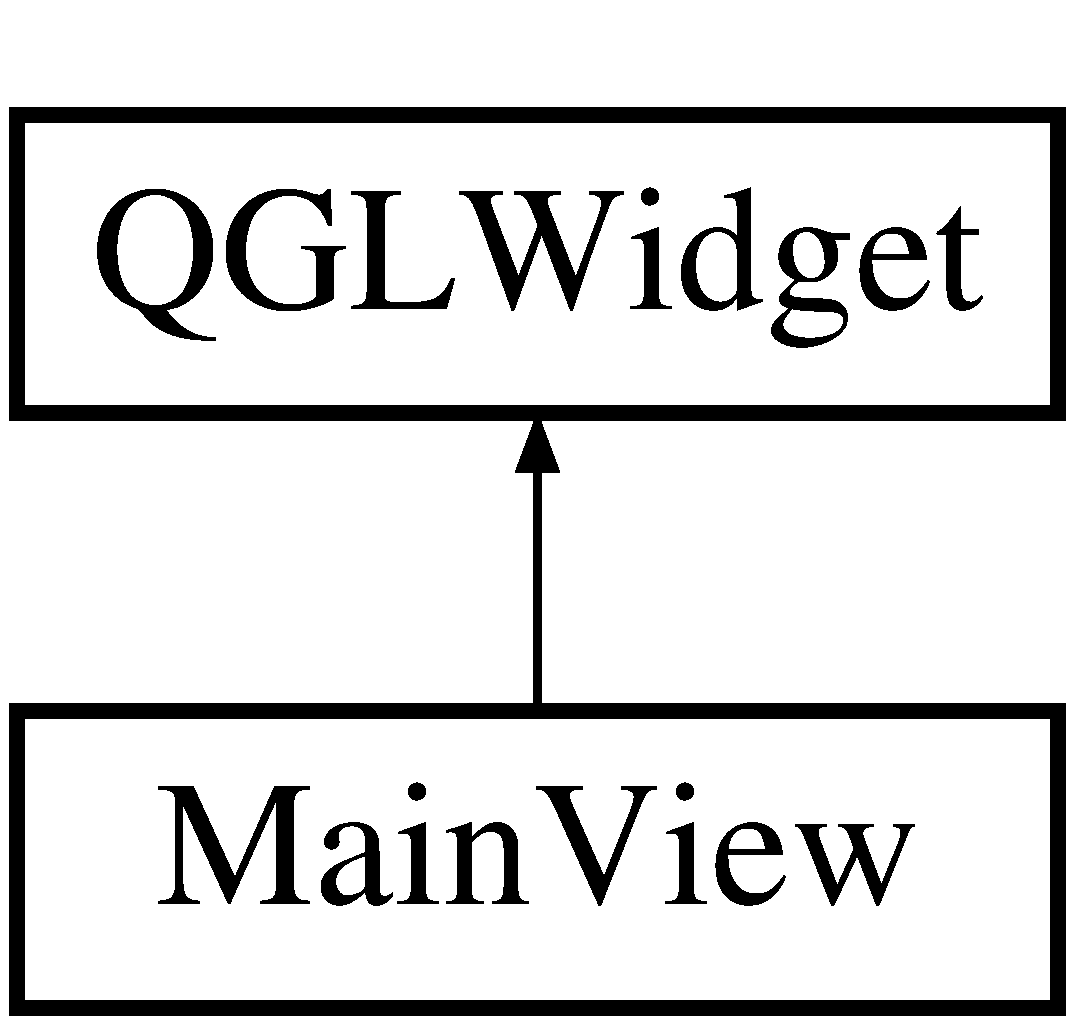
\includegraphics[height=2.000000cm]{class_main_view}
\end{center}
\end{figure}
\subsection*{Public Slots}
\begin{DoxyCompactItemize}
\item 
void \hyperlink{class_main_view_a456d4761f9c8dcf828ea4fcfac37c21a}{timer\+Update} ()
\item 
void \hyperlink{class_main_view_afbc772adcee43265ce364ff656c19500}{toggle\+Animation} ()
\item 
void \hyperlink{class_main_view_a8e1549cbc6edb92d9eedfeae3976f161}{take\+Screen\+Shot} ()
\end{DoxyCompactItemize}
\subsection*{Public Member Functions}
\begin{DoxyCompactItemize}
\item 
\hyperlink{class_main_view_a46ff460541fd6b9dfe75eeff6b78466a}{Main\+View} (const Q\+G\+L\+Format \&format, Q\+Widget $\ast$parent=0)
\begin{DoxyCompactList}\small\item\em Constructor of \hyperlink{class_main_view}{Main\+View}. \end{DoxyCompactList}\item 
void \hyperlink{class_main_view_a90f82be94e9397e1f12efbe1bd9dcc8a}{update\+Cube} (glm\+::vec3 p1, glm\+::vec3 p2)
\begin{DoxyCompactList}\small\item\em Update the models of the line and the cube. \end{DoxyCompactList}\item 
void \hyperlink{class_main_view_a4534f6ae9efa1c02922692dc06cc335a}{rotate\+Matrix} (\hyperlink{structset_of_values}{set\+Of\+Values} param)
\begin{DoxyCompactList}\small\item\em Do the transformations (translations and rotation) on the models. \end{DoxyCompactList}\item 
void \hyperlink{class_main_view_a3a3c5e12f747bb2226401c3cbd7618f6}{update\+Camera} (\hyperlink{structset_of_view}{set\+Of\+View} param)
\begin{DoxyCompactList}\small\item\em Update the camera. \end{DoxyCompactList}\item 
void \hyperlink{class_main_view_ad30cbdd44fc8711ec461bd268fe9d66a}{restore\+Camera} ()
\begin{DoxyCompactList}\small\item\em Restore the default parameters of the cube and the view. \end{DoxyCompactList}\end{DoxyCompactItemize}
\subsection*{Protected Member Functions}
\begin{DoxyCompactItemize}
\item 
void \hyperlink{class_main_view_aba66808352339bdf5f459d134181e4b0}{initialize\+GL} ()
\item 
void \hyperlink{class_main_view_a9b9be05c20817f6eb853bd58c406f0e0}{paint\+GL} ()
\item 
void \hyperlink{class_main_view_a8d8c7515e0a637a0db30608ebf489f1d}{resize\+GL} (int w, int h)
\end{DoxyCompactItemize}


\subsection{Detailed Description}
It is the main view, it will recover data and transmit them. 

\subsection{Constructor \& Destructor Documentation}
\hypertarget{class_main_view_a46ff460541fd6b9dfe75eeff6b78466a}{}\label{class_main_view_a46ff460541fd6b9dfe75eeff6b78466a} 
\index{Main\+View@{Main\+View}!Main\+View@{Main\+View}}
\index{Main\+View@{Main\+View}!Main\+View@{Main\+View}}
\subsubsection{\texorpdfstring{Main\+View()}{MainView()}}
{\footnotesize\ttfamily Main\+View\+::\+Main\+View (\begin{DoxyParamCaption}\item[{const Q\+G\+L\+Format \&}]{format,  }\item[{Q\+Widget $\ast$}]{parent = {\ttfamily 0} }\end{DoxyParamCaption})}



Constructor of \hyperlink{class_main_view}{Main\+View}. 


\begin{DoxyParams}{Parameters}
{\em format} & Specifies the display format of an Open\+GL rendering context. \\
\hline
{\em widget} & the global widget \\
\hline
\end{DoxyParams}


\subsection{Member Function Documentation}
\hypertarget{class_main_view_aba66808352339bdf5f459d134181e4b0}{}\label{class_main_view_aba66808352339bdf5f459d134181e4b0} 
\index{Main\+View@{Main\+View}!initialize\+GL@{initialize\+GL}}
\index{initialize\+GL@{initialize\+GL}!Main\+View@{Main\+View}}
\subsubsection{\texorpdfstring{initialize\+G\+L()}{initializeGL()}}
{\footnotesize\ttfamily void Main\+View\+::initialize\+GL (\begin{DoxyParamCaption}{ }\end{DoxyParamCaption})\hspace{0.3cm}{\ttfamily [protected]}}

Initialize \hypertarget{class_main_view_a9b9be05c20817f6eb853bd58c406f0e0}{}\label{class_main_view_a9b9be05c20817f6eb853bd58c406f0e0} 
\index{Main\+View@{Main\+View}!paint\+GL@{paint\+GL}}
\index{paint\+GL@{paint\+GL}!Main\+View@{Main\+View}}
\subsubsection{\texorpdfstring{paint\+G\+L()}{paintGL()}}
{\footnotesize\ttfamily void Main\+View\+::paint\+GL (\begin{DoxyParamCaption}{ }\end{DoxyParamCaption})\hspace{0.3cm}{\ttfamily [protected]}}

Paint \hypertarget{class_main_view_a8d8c7515e0a637a0db30608ebf489f1d}{}\label{class_main_view_a8d8c7515e0a637a0db30608ebf489f1d} 
\index{Main\+View@{Main\+View}!resize\+GL@{resize\+GL}}
\index{resize\+GL@{resize\+GL}!Main\+View@{Main\+View}}
\subsubsection{\texorpdfstring{resize\+G\+L()}{resizeGL()}}
{\footnotesize\ttfamily void Main\+View\+::resize\+GL (\begin{DoxyParamCaption}\item[{int}]{w,  }\item[{int}]{h }\end{DoxyParamCaption})\hspace{0.3cm}{\ttfamily [protected]}}

Resize \hypertarget{class_main_view_ad30cbdd44fc8711ec461bd268fe9d66a}{}\label{class_main_view_ad30cbdd44fc8711ec461bd268fe9d66a} 
\index{Main\+View@{Main\+View}!restore\+Camera@{restore\+Camera}}
\index{restore\+Camera@{restore\+Camera}!Main\+View@{Main\+View}}
\subsubsection{\texorpdfstring{restore\+Camera()}{restoreCamera()}}
{\footnotesize\ttfamily void Main\+View\+::restore\+Camera (\begin{DoxyParamCaption}{ }\end{DoxyParamCaption})}



Restore the default parameters of the cube and the view. 

\hypertarget{class_main_view_a4534f6ae9efa1c02922692dc06cc335a}{}\label{class_main_view_a4534f6ae9efa1c02922692dc06cc335a} 
\index{Main\+View@{Main\+View}!rotate\+Matrix@{rotate\+Matrix}}
\index{rotate\+Matrix@{rotate\+Matrix}!Main\+View@{Main\+View}}
\subsubsection{\texorpdfstring{rotate\+Matrix()}{rotateMatrix()}}
{\footnotesize\ttfamily void Main\+View\+::rotate\+Matrix (\begin{DoxyParamCaption}\item[{\hyperlink{structset_of_values}{set\+Of\+Values}}]{param }\end{DoxyParamCaption})}



Do the transformations (translations and rotation) on the models. 


\begin{DoxyParams}{Parameters}
{\em param} & set of values from the user \\
\hline
\end{DoxyParams}
\hypertarget{class_main_view_a8e1549cbc6edb92d9eedfeae3976f161}{}\label{class_main_view_a8e1549cbc6edb92d9eedfeae3976f161} 
\index{Main\+View@{Main\+View}!take\+Screen\+Shot@{take\+Screen\+Shot}}
\index{take\+Screen\+Shot@{take\+Screen\+Shot}!Main\+View@{Main\+View}}
\subsubsection{\texorpdfstring{take\+Screen\+Shot}{takeScreenShot}}
{\footnotesize\ttfamily void Main\+View\+::take\+Screen\+Shot (\begin{DoxyParamCaption}{ }\end{DoxyParamCaption})\hspace{0.3cm}{\ttfamily [slot]}}

Slot which allow us to do a screenshot \hypertarget{class_main_view_a456d4761f9c8dcf828ea4fcfac37c21a}{}\label{class_main_view_a456d4761f9c8dcf828ea4fcfac37c21a} 
\index{Main\+View@{Main\+View}!timer\+Update@{timer\+Update}}
\index{timer\+Update@{timer\+Update}!Main\+View@{Main\+View}}
\subsubsection{\texorpdfstring{timer\+Update}{timerUpdate}}
{\footnotesize\ttfamily void Main\+View\+::timer\+Update (\begin{DoxyParamCaption}{ }\end{DoxyParamCaption})\hspace{0.3cm}{\ttfamily [slot]}}

Slot wich update the timer \hypertarget{class_main_view_afbc772adcee43265ce364ff656c19500}{}\label{class_main_view_afbc772adcee43265ce364ff656c19500} 
\index{Main\+View@{Main\+View}!toggle\+Animation@{toggle\+Animation}}
\index{toggle\+Animation@{toggle\+Animation}!Main\+View@{Main\+View}}
\subsubsection{\texorpdfstring{toggle\+Animation}{toggleAnimation}}
{\footnotesize\ttfamily void Main\+View\+::toggle\+Animation (\begin{DoxyParamCaption}{ }\end{DoxyParamCaption})\hspace{0.3cm}{\ttfamily [slot]}}

Slot which deals with animations \hypertarget{class_main_view_a3a3c5e12f747bb2226401c3cbd7618f6}{}\label{class_main_view_a3a3c5e12f747bb2226401c3cbd7618f6} 
\index{Main\+View@{Main\+View}!update\+Camera@{update\+Camera}}
\index{update\+Camera@{update\+Camera}!Main\+View@{Main\+View}}
\subsubsection{\texorpdfstring{update\+Camera()}{updateCamera()}}
{\footnotesize\ttfamily void Main\+View\+::update\+Camera (\begin{DoxyParamCaption}\item[{\hyperlink{structset_of_view}{set\+Of\+View}}]{param }\end{DoxyParamCaption})}



Update the camera. 


\begin{DoxyParams}{Parameters}
{\em param} & set of values of the view from the user \\
\hline
\end{DoxyParams}
\hypertarget{class_main_view_a90f82be94e9397e1f12efbe1bd9dcc8a}{}\label{class_main_view_a90f82be94e9397e1f12efbe1bd9dcc8a} 
\index{Main\+View@{Main\+View}!update\+Cube@{update\+Cube}}
\index{update\+Cube@{update\+Cube}!Main\+View@{Main\+View}}
\subsubsection{\texorpdfstring{update\+Cube()}{updateCube()}}
{\footnotesize\ttfamily void Main\+View\+::update\+Cube (\begin{DoxyParamCaption}\item[{glm\+::vec3}]{p1,  }\item[{glm\+::vec3}]{p2 }\end{DoxyParamCaption})}



Update the models of the line and the cube. 


\begin{DoxyParams}{Parameters}
{\em p1} & point 1 of the line \\
\hline
{\em p1} & point 1 of the line \\
\hline
\end{DoxyParams}


The documentation for this class was generated from the following files\+:\begin{DoxyCompactItemize}
\item 
D\+:/\+Q\+T\+\_\+projets/\+Cube\+Menu/\hyperlink{mainview_8h}{mainview.\+h}\item 
D\+:/\+Q\+T\+\_\+projets/\+Cube\+Menu/\hyperlink{mainview_8cpp}{mainview.\+cpp}\end{DoxyCompactItemize}

\hypertarget{class_ui_1_1_main_window}{}\section{Ui\+:\+:Main\+Window Class Reference}
\label{class_ui_1_1_main_window}\index{Ui\+::\+Main\+Window@{Ui\+::\+Main\+Window}}


{\ttfamily \#include $<$ui\+\_\+mainwindow.\+h$>$}

Inheritance diagram for Ui\+:\+:Main\+Window\+:\begin{figure}[H]
\begin{center}
\leavevmode
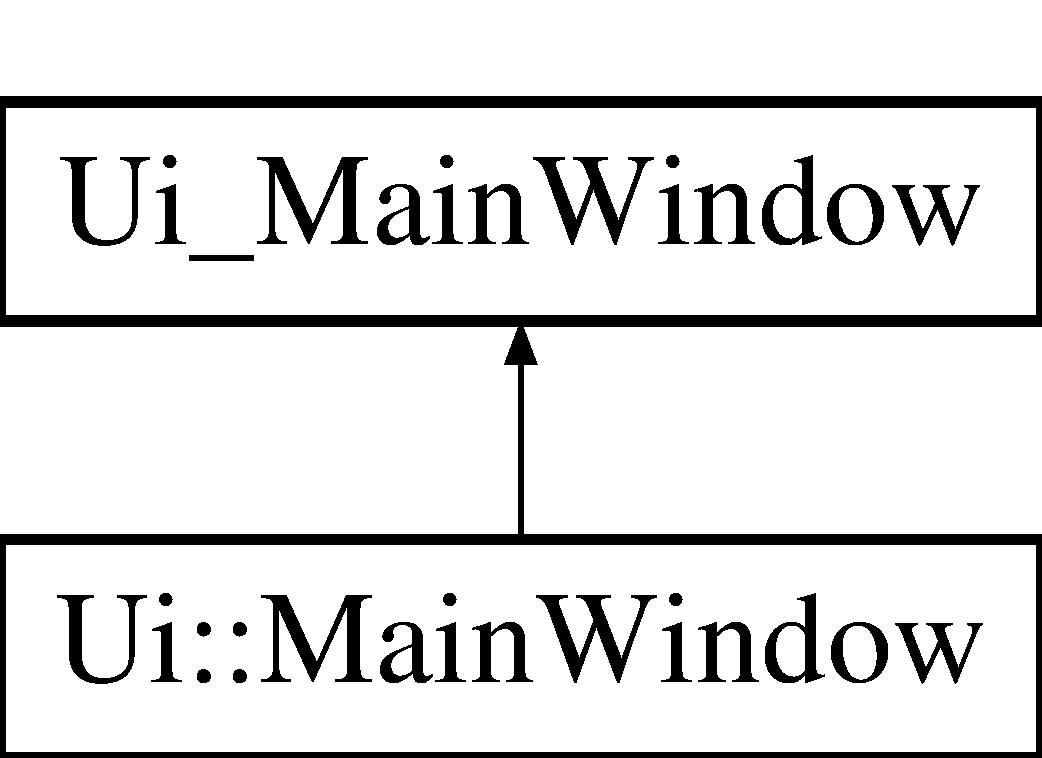
\includegraphics[height=2.000000cm]{class_ui_1_1_main_window}
\end{center}
\end{figure}
\subsection*{Additional Inherited Members}


The documentation for this class was generated from the following file\+:\begin{DoxyCompactItemize}
\item 
D\+:/\+Q\+T\+\_\+projets/\+Cube\+Menu/\hyperlink{ui__mainwindow_8h}{ui\+\_\+mainwindow.\+h}\end{DoxyCompactItemize}

\hypertarget{class_main_window}{}\section{Main\+Window Class Reference}
\label{class_main_window}\index{Main\+Window@{Main\+Window}}


It is the main window, where the user can choose parameters.  




{\ttfamily \#include $<$mainwindow.\+h$>$}

Inheritance diagram for Main\+Window\+:\begin{figure}[H]
\begin{center}
\leavevmode
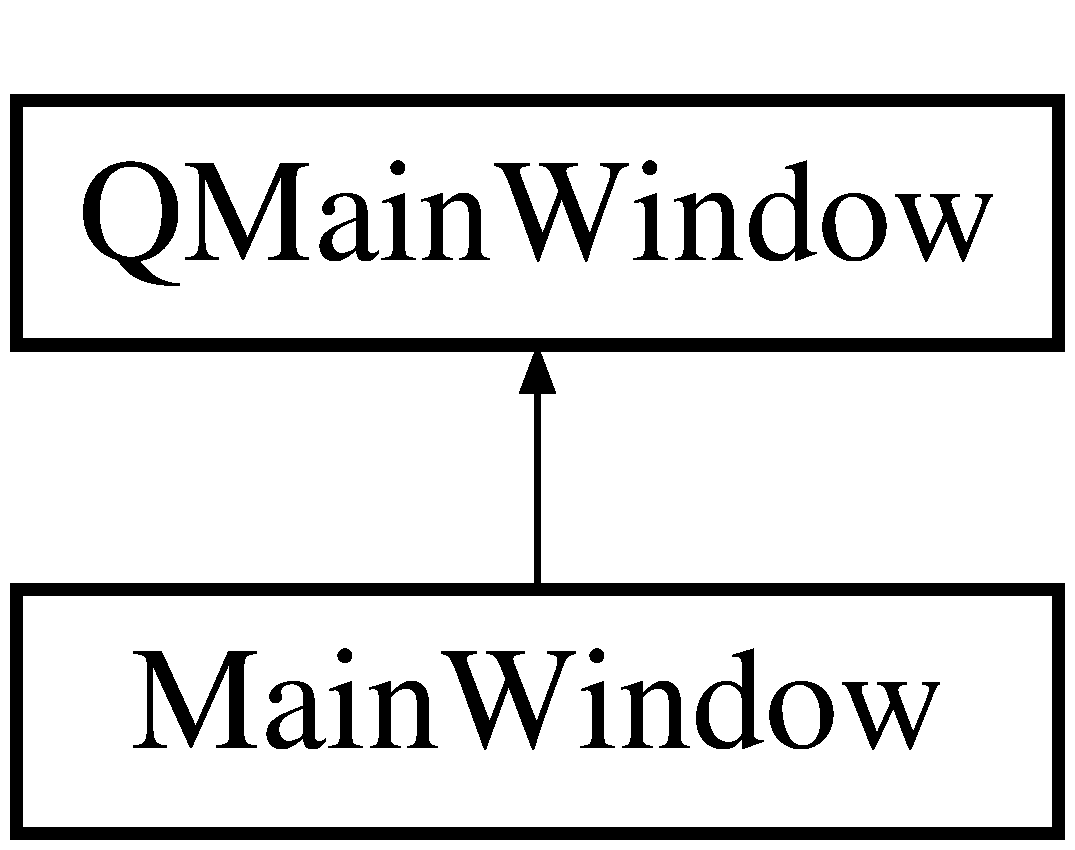
\includegraphics[height=2.000000cm]{class_main_window}
\end{center}
\end{figure}
\subsection*{Public Member Functions}
\begin{DoxyCompactItemize}
\item 
\hyperlink{class_main_window_a8b244be8b7b7db1b08de2a2acb9409db}{Main\+Window} (Q\+Widget $\ast$parent=0)
\begin{DoxyCompactList}\small\item\em Constructor of \hyperlink{class_main_window}{Main\+Window}. \end{DoxyCompactList}\item 
void \hyperlink{class_main_window_adffbce021ec28108d1b1893bf43da5e0}{set\+View} (\hyperlink{class_main_view}{Main\+View} $\ast$view)
\begin{DoxyCompactList}\small\item\em Set the Mainview of the project. \end{DoxyCompactList}\item 
\hyperlink{class_main_window_ae98d00a93bc118200eeef9f9bba1dba7}{$\sim$\+Main\+Window} ()
\begin{DoxyCompactList}\small\item\em Default destructor of \hyperlink{class_main_window}{Main\+Window}. \end{DoxyCompactList}\end{DoxyCompactItemize}


\subsection{Detailed Description}
It is the main window, where the user can choose parameters. 

\subsection{Constructor \& Destructor Documentation}
\hypertarget{class_main_window_a8b244be8b7b7db1b08de2a2acb9409db}{}\label{class_main_window_a8b244be8b7b7db1b08de2a2acb9409db} 
\index{Main\+Window@{Main\+Window}!Main\+Window@{Main\+Window}}
\index{Main\+Window@{Main\+Window}!Main\+Window@{Main\+Window}}
\subsubsection{\texorpdfstring{Main\+Window()}{MainWindow()}}
{\footnotesize\ttfamily Main\+Window\+::\+Main\+Window (\begin{DoxyParamCaption}\item[{Q\+Widget $\ast$}]{parent = {\ttfamily 0} }\end{DoxyParamCaption})\hspace{0.3cm}{\ttfamily [explicit]}}



Constructor of \hyperlink{class_main_window}{Main\+Window}. 


\begin{DoxyParams}{Parameters}
{\em parent} & the global widget \\
\hline
\end{DoxyParams}
\hypertarget{class_main_window_ae98d00a93bc118200eeef9f9bba1dba7}{}\label{class_main_window_ae98d00a93bc118200eeef9f9bba1dba7} 
\index{Main\+Window@{Main\+Window}!````~Main\+Window@{$\sim$\+Main\+Window}}
\index{````~Main\+Window@{$\sim$\+Main\+Window}!Main\+Window@{Main\+Window}}
\subsubsection{\texorpdfstring{$\sim$\+Main\+Window()}{~MainWindow()}}
{\footnotesize\ttfamily Main\+Window\+::$\sim$\+Main\+Window (\begin{DoxyParamCaption}{ }\end{DoxyParamCaption})}



Default destructor of \hyperlink{class_main_window}{Main\+Window}. 



\subsection{Member Function Documentation}
\hypertarget{class_main_window_adffbce021ec28108d1b1893bf43da5e0}{}\label{class_main_window_adffbce021ec28108d1b1893bf43da5e0} 
\index{Main\+Window@{Main\+Window}!set\+View@{set\+View}}
\index{set\+View@{set\+View}!Main\+Window@{Main\+Window}}
\subsubsection{\texorpdfstring{set\+View()}{setView()}}
{\footnotesize\ttfamily void Main\+Window\+::set\+View (\begin{DoxyParamCaption}\item[{\hyperlink{class_main_view}{Main\+View} $\ast$}]{view }\end{DoxyParamCaption})}



Set the Mainview of the project. 


\begin{DoxyParams}{Parameters}
{\em view} & Mainview \\
\hline
\end{DoxyParams}


The documentation for this class was generated from the following files\+:\begin{DoxyCompactItemize}
\item 
D\+:/\+Q\+T\+\_\+projets/\+Cube\+Menu/\hyperlink{mainwindow_8h}{mainwindow.\+h}\item 
D\+:/\+Q\+T\+\_\+projets/\+Cube\+Menu/\hyperlink{mainwindow_8cpp}{mainwindow.\+cpp}\end{DoxyCompactItemize}

\hypertarget{structqt__meta__stringdata___dialog__t}{}\section{qt\+\_\+meta\+\_\+stringdata\+\_\+\+Dialog\+\_\+t Struct Reference}
\label{structqt__meta__stringdata___dialog__t}\index{qt\+\_\+meta\+\_\+stringdata\+\_\+\+Dialog\+\_\+t@{qt\+\_\+meta\+\_\+stringdata\+\_\+\+Dialog\+\_\+t}}
\subsection*{Public Attributes}
\begin{DoxyCompactItemize}
\item 
Q\+Byte\+Array\+Data \hyperlink{structqt__meta__stringdata___dialog__t_a8d4d74626c71b087b6b991b787f5368e}{data} \mbox{[}5\mbox{]}
\item 
char \hyperlink{structqt__meta__stringdata___dialog__t_af93413df8f81b853970c266cdb3d8869}{stringdata0} \mbox{[}74\mbox{]}
\end{DoxyCompactItemize}


\subsection{Member Data Documentation}
\hypertarget{structqt__meta__stringdata___dialog__t_a8d4d74626c71b087b6b991b787f5368e}{}\label{structqt__meta__stringdata___dialog__t_a8d4d74626c71b087b6b991b787f5368e} 
\index{qt\+\_\+meta\+\_\+stringdata\+\_\+\+Dialog\+\_\+t@{qt\+\_\+meta\+\_\+stringdata\+\_\+\+Dialog\+\_\+t}!data@{data}}
\index{data@{data}!qt\+\_\+meta\+\_\+stringdata\+\_\+\+Dialog\+\_\+t@{qt\+\_\+meta\+\_\+stringdata\+\_\+\+Dialog\+\_\+t}}
\subsubsection{\texorpdfstring{data}{data}}
{\footnotesize\ttfamily Q\+Byte\+Array\+Data qt\+\_\+meta\+\_\+stringdata\+\_\+\+Dialog\+\_\+t\+::data}

\hypertarget{structqt__meta__stringdata___dialog__t_af93413df8f81b853970c266cdb3d8869}{}\label{structqt__meta__stringdata___dialog__t_af93413df8f81b853970c266cdb3d8869} 
\index{qt\+\_\+meta\+\_\+stringdata\+\_\+\+Dialog\+\_\+t@{qt\+\_\+meta\+\_\+stringdata\+\_\+\+Dialog\+\_\+t}!stringdata0@{stringdata0}}
\index{stringdata0@{stringdata0}!qt\+\_\+meta\+\_\+stringdata\+\_\+\+Dialog\+\_\+t@{qt\+\_\+meta\+\_\+stringdata\+\_\+\+Dialog\+\_\+t}}
\subsubsection{\texorpdfstring{stringdata0}{stringdata0}}
{\footnotesize\ttfamily char qt\+\_\+meta\+\_\+stringdata\+\_\+\+Dialog\+\_\+t\+::stringdata0}



The documentation for this struct was generated from the following file\+:\begin{DoxyCompactItemize}
\item 
D\+:/\+Q\+T\+\_\+projets/\+Cube\+Menu/debug/\hyperlink{debug_2moc__dialog_8cpp}{moc\+\_\+dialog.\+cpp}\end{DoxyCompactItemize}

\hypertarget{structqt__meta__stringdata___dialog__view__t}{}\section{qt\+\_\+meta\+\_\+stringdata\+\_\+\+Dialog\+\_\+view\+\_\+t Struct Reference}
\label{structqt__meta__stringdata___dialog__view__t}\index{qt\+\_\+meta\+\_\+stringdata\+\_\+\+Dialog\+\_\+view\+\_\+t@{qt\+\_\+meta\+\_\+stringdata\+\_\+\+Dialog\+\_\+view\+\_\+t}}
\subsection*{Public Attributes}
\begin{DoxyCompactItemize}
\item 
Q\+Byte\+Array\+Data \hyperlink{structqt__meta__stringdata___dialog__view__t_adce2bfd7d9c5d652c6a42fcefaf98219}{data} \mbox{[}3\mbox{]}
\item 
char \hyperlink{structqt__meta__stringdata___dialog__view__t_a9c929253a0c00e3ba615ee5244832dd9}{stringdata0} \mbox{[}34\mbox{]}
\end{DoxyCompactItemize}


\subsection{Member Data Documentation}
\hypertarget{structqt__meta__stringdata___dialog__view__t_adce2bfd7d9c5d652c6a42fcefaf98219}{}\label{structqt__meta__stringdata___dialog__view__t_adce2bfd7d9c5d652c6a42fcefaf98219} 
\index{qt\+\_\+meta\+\_\+stringdata\+\_\+\+Dialog\+\_\+view\+\_\+t@{qt\+\_\+meta\+\_\+stringdata\+\_\+\+Dialog\+\_\+view\+\_\+t}!data@{data}}
\index{data@{data}!qt\+\_\+meta\+\_\+stringdata\+\_\+\+Dialog\+\_\+view\+\_\+t@{qt\+\_\+meta\+\_\+stringdata\+\_\+\+Dialog\+\_\+view\+\_\+t}}
\subsubsection{\texorpdfstring{data}{data}}
{\footnotesize\ttfamily Q\+Byte\+Array\+Data qt\+\_\+meta\+\_\+stringdata\+\_\+\+Dialog\+\_\+view\+\_\+t\+::data\mbox{[}3\mbox{]}}

\hypertarget{structqt__meta__stringdata___dialog__view__t_a9c929253a0c00e3ba615ee5244832dd9}{}\label{structqt__meta__stringdata___dialog__view__t_a9c929253a0c00e3ba615ee5244832dd9} 
\index{qt\+\_\+meta\+\_\+stringdata\+\_\+\+Dialog\+\_\+view\+\_\+t@{qt\+\_\+meta\+\_\+stringdata\+\_\+\+Dialog\+\_\+view\+\_\+t}!stringdata0@{stringdata0}}
\index{stringdata0@{stringdata0}!qt\+\_\+meta\+\_\+stringdata\+\_\+\+Dialog\+\_\+view\+\_\+t@{qt\+\_\+meta\+\_\+stringdata\+\_\+\+Dialog\+\_\+view\+\_\+t}}
\subsubsection{\texorpdfstring{stringdata0}{stringdata0}}
{\footnotesize\ttfamily char qt\+\_\+meta\+\_\+stringdata\+\_\+\+Dialog\+\_\+view\+\_\+t\+::stringdata0\mbox{[}34\mbox{]}}



The documentation for this struct was generated from the following file\+:\begin{DoxyCompactItemize}
\item 
D\+:/\+Q\+T\+\_\+projets/\+Cube\+Menu/debug/\hyperlink{moc__dialog__view_8cpp}{moc\+\_\+dialog\+\_\+view.\+cpp}\end{DoxyCompactItemize}

\hypertarget{structqt__meta__stringdata___dialog_eyes__t}{}\section{qt\+\_\+meta\+\_\+stringdata\+\_\+\+Dialog\+Eyes\+\_\+t Struct Reference}
\label{structqt__meta__stringdata___dialog_eyes__t}\index{qt\+\_\+meta\+\_\+stringdata\+\_\+\+Dialog\+Eyes\+\_\+t@{qt\+\_\+meta\+\_\+stringdata\+\_\+\+Dialog\+Eyes\+\_\+t}}
\subsection*{Public Attributes}
\begin{DoxyCompactItemize}
\item 
Q\+Byte\+Array\+Data \hyperlink{structqt__meta__stringdata___dialog_eyes__t_ad659505232893d9249a61e4ea0d9628a}{data} \mbox{[}5\mbox{]}
\item 
char \hyperlink{structqt__meta__stringdata___dialog_eyes__t_a1ad6dad721de3132170d24f2879ce8c8}{stringdata0} \mbox{[}84\mbox{]}
\end{DoxyCompactItemize}


\subsection{Member Data Documentation}
\hypertarget{structqt__meta__stringdata___dialog_eyes__t_ad659505232893d9249a61e4ea0d9628a}{}\label{structqt__meta__stringdata___dialog_eyes__t_ad659505232893d9249a61e4ea0d9628a} 
\index{qt\+\_\+meta\+\_\+stringdata\+\_\+\+Dialog\+Eyes\+\_\+t@{qt\+\_\+meta\+\_\+stringdata\+\_\+\+Dialog\+Eyes\+\_\+t}!data@{data}}
\index{data@{data}!qt\+\_\+meta\+\_\+stringdata\+\_\+\+Dialog\+Eyes\+\_\+t@{qt\+\_\+meta\+\_\+stringdata\+\_\+\+Dialog\+Eyes\+\_\+t}}
\subsubsection{\texorpdfstring{data}{data}}
{\footnotesize\ttfamily Q\+Byte\+Array\+Data qt\+\_\+meta\+\_\+stringdata\+\_\+\+Dialog\+Eyes\+\_\+t\+::data}

\hypertarget{structqt__meta__stringdata___dialog_eyes__t_a1ad6dad721de3132170d24f2879ce8c8}{}\label{structqt__meta__stringdata___dialog_eyes__t_a1ad6dad721de3132170d24f2879ce8c8} 
\index{qt\+\_\+meta\+\_\+stringdata\+\_\+\+Dialog\+Eyes\+\_\+t@{qt\+\_\+meta\+\_\+stringdata\+\_\+\+Dialog\+Eyes\+\_\+t}!stringdata0@{stringdata0}}
\index{stringdata0@{stringdata0}!qt\+\_\+meta\+\_\+stringdata\+\_\+\+Dialog\+Eyes\+\_\+t@{qt\+\_\+meta\+\_\+stringdata\+\_\+\+Dialog\+Eyes\+\_\+t}}
\subsubsection{\texorpdfstring{stringdata0}{stringdata0}}
{\footnotesize\ttfamily char qt\+\_\+meta\+\_\+stringdata\+\_\+\+Dialog\+Eyes\+\_\+t\+::stringdata0}



The documentation for this struct was generated from the following file\+:\begin{DoxyCompactItemize}
\item 
D\+:/\+Q\+T\+\_\+projets/\+Cube\+Menu/debug/\hyperlink{debug_2moc__dialogeyes_8cpp}{moc\+\_\+dialogeyes.\+cpp}\end{DoxyCompactItemize}

\hypertarget{structqt__meta__stringdata___main_view__t}{}\section{qt\+\_\+meta\+\_\+stringdata\+\_\+\+Main\+View\+\_\+t Struct Reference}
\label{structqt__meta__stringdata___main_view__t}\index{qt\+\_\+meta\+\_\+stringdata\+\_\+\+Main\+View\+\_\+t@{qt\+\_\+meta\+\_\+stringdata\+\_\+\+Main\+View\+\_\+t}}
\subsection*{Public Attributes}
\begin{DoxyCompactItemize}
\item 
Q\+Byte\+Array\+Data \hyperlink{structqt__meta__stringdata___main_view__t_a3eef91355782fab250988585fdf2e5ad}{data} \mbox{[}5\mbox{]}
\item 
char \hyperlink{structqt__meta__stringdata___main_view__t_abc5243f08f83cd082d01bf06a4c01e34}{stringdata0} \mbox{[}53\mbox{]}
\end{DoxyCompactItemize}


\subsection{Member Data Documentation}
\hypertarget{structqt__meta__stringdata___main_view__t_a3eef91355782fab250988585fdf2e5ad}{}\label{structqt__meta__stringdata___main_view__t_a3eef91355782fab250988585fdf2e5ad} 
\index{qt\+\_\+meta\+\_\+stringdata\+\_\+\+Main\+View\+\_\+t@{qt\+\_\+meta\+\_\+stringdata\+\_\+\+Main\+View\+\_\+t}!data@{data}}
\index{data@{data}!qt\+\_\+meta\+\_\+stringdata\+\_\+\+Main\+View\+\_\+t@{qt\+\_\+meta\+\_\+stringdata\+\_\+\+Main\+View\+\_\+t}}
\subsubsection{\texorpdfstring{data}{data}}
{\footnotesize\ttfamily Q\+Byte\+Array\+Data qt\+\_\+meta\+\_\+stringdata\+\_\+\+Main\+View\+\_\+t\+::data}

\hypertarget{structqt__meta__stringdata___main_view__t_abc5243f08f83cd082d01bf06a4c01e34}{}\label{structqt__meta__stringdata___main_view__t_abc5243f08f83cd082d01bf06a4c01e34} 
\index{qt\+\_\+meta\+\_\+stringdata\+\_\+\+Main\+View\+\_\+t@{qt\+\_\+meta\+\_\+stringdata\+\_\+\+Main\+View\+\_\+t}!stringdata0@{stringdata0}}
\index{stringdata0@{stringdata0}!qt\+\_\+meta\+\_\+stringdata\+\_\+\+Main\+View\+\_\+t@{qt\+\_\+meta\+\_\+stringdata\+\_\+\+Main\+View\+\_\+t}}
\subsubsection{\texorpdfstring{stringdata0}{stringdata0}}
{\footnotesize\ttfamily char qt\+\_\+meta\+\_\+stringdata\+\_\+\+Main\+View\+\_\+t\+::stringdata0}



The documentation for this struct was generated from the following file\+:\begin{DoxyCompactItemize}
\item 
D\+:/\+Q\+T\+\_\+projets/\+Cube\+Menu/debug/\hyperlink{debug_2moc__mainview_8cpp}{moc\+\_\+mainview.\+cpp}\end{DoxyCompactItemize}

\hypertarget{structqt__meta__stringdata___main_window__t}{}\section{qt\+\_\+meta\+\_\+stringdata\+\_\+\+Main\+Window\+\_\+t Struct Reference}
\label{structqt__meta__stringdata___main_window__t}\index{qt\+\_\+meta\+\_\+stringdata\+\_\+\+Main\+Window\+\_\+t@{qt\+\_\+meta\+\_\+stringdata\+\_\+\+Main\+Window\+\_\+t}}
\subsection*{Public Attributes}
\begin{DoxyCompactItemize}
\item 
Q\+Byte\+Array\+Data \hyperlink{structqt__meta__stringdata___main_window__t_a092956d0ba2e51cd73092e8a5ebb6ce6}{data} \mbox{[}8\mbox{]}
\item 
char \hyperlink{structqt__meta__stringdata___main_window__t_a88959992f1140a84ca21ab555f0345a1}{stringdata0} \mbox{[}225\mbox{]}
\end{DoxyCompactItemize}


\subsection{Member Data Documentation}
\hypertarget{structqt__meta__stringdata___main_window__t_a092956d0ba2e51cd73092e8a5ebb6ce6}{}\label{structqt__meta__stringdata___main_window__t_a092956d0ba2e51cd73092e8a5ebb6ce6} 
\index{qt\+\_\+meta\+\_\+stringdata\+\_\+\+Main\+Window\+\_\+t@{qt\+\_\+meta\+\_\+stringdata\+\_\+\+Main\+Window\+\_\+t}!data@{data}}
\index{data@{data}!qt\+\_\+meta\+\_\+stringdata\+\_\+\+Main\+Window\+\_\+t@{qt\+\_\+meta\+\_\+stringdata\+\_\+\+Main\+Window\+\_\+t}}
\subsubsection{\texorpdfstring{data}{data}}
{\footnotesize\ttfamily Q\+Byte\+Array\+Data qt\+\_\+meta\+\_\+stringdata\+\_\+\+Main\+Window\+\_\+t\+::data}

\hypertarget{structqt__meta__stringdata___main_window__t_a88959992f1140a84ca21ab555f0345a1}{}\label{structqt__meta__stringdata___main_window__t_a88959992f1140a84ca21ab555f0345a1} 
\index{qt\+\_\+meta\+\_\+stringdata\+\_\+\+Main\+Window\+\_\+t@{qt\+\_\+meta\+\_\+stringdata\+\_\+\+Main\+Window\+\_\+t}!stringdata0@{stringdata0}}
\index{stringdata0@{stringdata0}!qt\+\_\+meta\+\_\+stringdata\+\_\+\+Main\+Window\+\_\+t@{qt\+\_\+meta\+\_\+stringdata\+\_\+\+Main\+Window\+\_\+t}}
\subsubsection{\texorpdfstring{stringdata0}{stringdata0}}
{\footnotesize\ttfamily char qt\+\_\+meta\+\_\+stringdata\+\_\+\+Main\+Window\+\_\+t\+::stringdata0}



The documentation for this struct was generated from the following file\+:\begin{DoxyCompactItemize}
\item 
D\+:/\+Q\+T\+\_\+projets/\+Cube\+Menu/debug/\hyperlink{debug_2moc__mainwindow_8cpp}{moc\+\_\+mainwindow.\+cpp}\end{DoxyCompactItemize}

\hypertarget{class_scene}{}\section{Scene Class Reference}
\label{class_scene}\index{Scene@{Scene}}


{\ttfamily \#include $<$scene.\+h$>$}

Inheritance diagram for Scene\+:\begin{figure}[H]
\begin{center}
\leavevmode
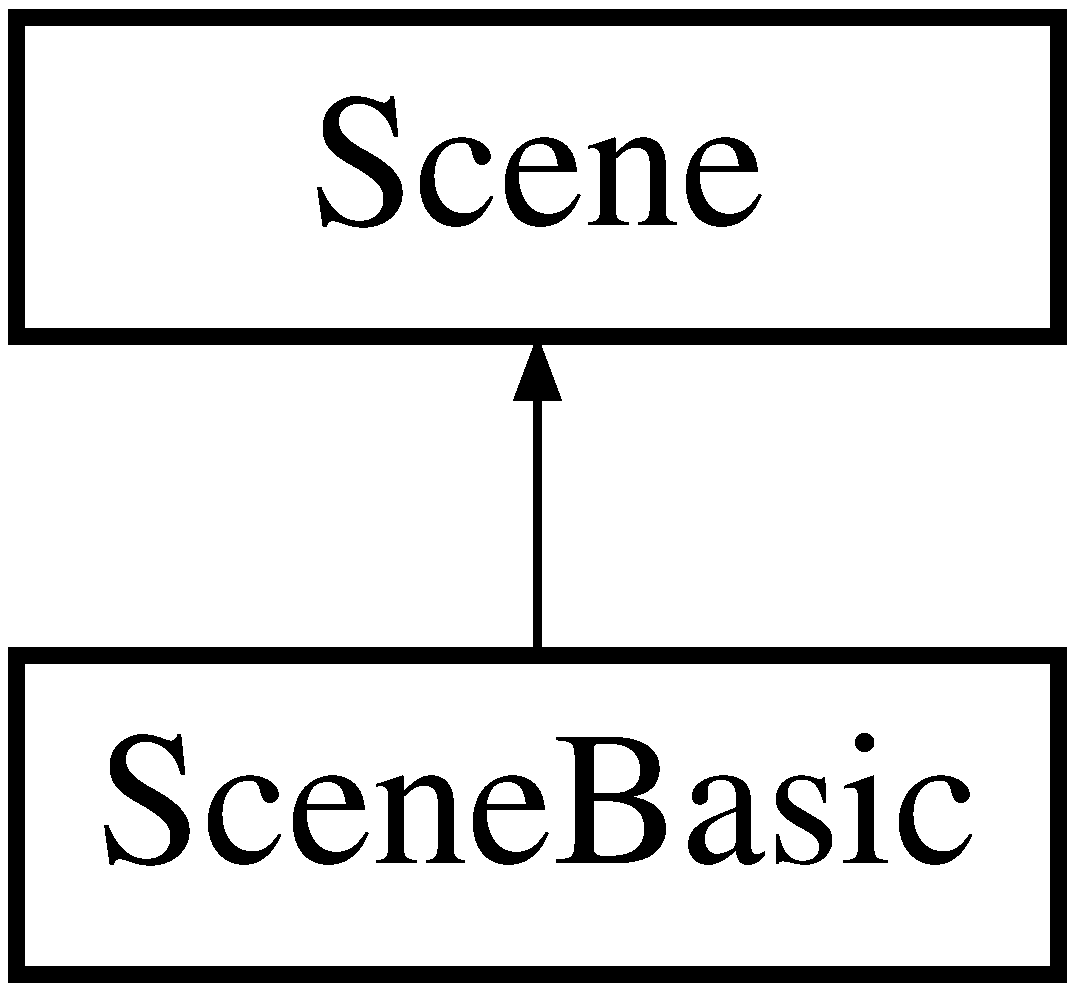
\includegraphics[height=2.000000cm]{class_scene}
\end{center}
\end{figure}
\subsection*{Public Member Functions}
\begin{DoxyCompactItemize}
\item 
virtual void \hyperlink{class_scene_ae76b830c1156bb40bd744afb63776be2}{init\+Scene} ()=0
\item 
virtual void \hyperlink{class_scene_aafa9ccf4d019005fdd41672afd13a7a9}{update} (float t)=0
\item 
virtual void \hyperlink{class_scene_a823f4cd60d27932ee16f74adb0421ff6}{render} ()=0
\item 
virtual void \hyperlink{class_scene_a454bd0a09c125201fbb32e15d4f62fa3}{resize} (int, int)=0
\item 
virtual void \hyperlink{class_scene_ab0c59864d813f7d11a2d362acfdd0e26}{set\+Angle\+Axis} (float angle, vec3 axis)=0
\item 
virtual void \hyperlink{class_scene_a0813a564a23d9a2d0a965d5bf422c1fd}{write\+Line} (glm\+::vec3 p1, glm\+::vec3 p2)=0
\item 
virtual void \hyperlink{class_scene_a2e371aa848e8c30f593c2d9a2687dd28}{Create\+V\+B\+O\+Line} ()=0
\item 
virtual void \hyperlink{class_scene_af0c5ec79be9fbb4a6a2554ac4aaaf473}{rotate\+Model} (\hyperlink{structset_of_values}{set\+Of\+Values} param)=0
\item 
virtual void \hyperlink{class_scene_a04ae3637cb26c4ad95004372d5a63654}{update\+Eye\+Camera\+On\+Cube} (std\+::vector$<$ double $>$ center)=0
\item 
virtual void \hyperlink{class_scene_a52181459b75a0c2f4706a26f3e200ca1}{update\+Eye\+Camera\+User} (\hyperlink{structset_of_view}{set\+Of\+View} param)=0
\item 
virtual void \hyperlink{class_scene_a74dc104a3f44abf1f09d7b627c9baa36}{restore\+Cam\+Default} ()=0
\item 
virtual std\+::vector$<$ double $>$ const  \& \hyperlink{class_scene_a15d25044dbd65a8d7d0759888fcd55a1}{get\+Center} ()=0
\end{DoxyCompactItemize}


\subsection{Member Function Documentation}
\hypertarget{class_scene_a2e371aa848e8c30f593c2d9a2687dd28}{}\label{class_scene_a2e371aa848e8c30f593c2d9a2687dd28} 
\index{Scene@{Scene}!Create\+V\+B\+O\+Line@{Create\+V\+B\+O\+Line}}
\index{Create\+V\+B\+O\+Line@{Create\+V\+B\+O\+Line}!Scene@{Scene}}
\subsubsection{\texorpdfstring{Create\+V\+B\+O\+Line()}{CreateVBOLine()}}
{\footnotesize\ttfamily virtual void Scene\+::\+Create\+V\+B\+O\+Line (\begin{DoxyParamCaption}{ }\end{DoxyParamCaption})\hspace{0.3cm}{\ttfamily [pure virtual]}}



Implemented in \hyperlink{class_scene_basic_ac0cc945b040983d7527cda36963ec711}{Scene\+Basic}.

\hypertarget{class_scene_a15d25044dbd65a8d7d0759888fcd55a1}{}\label{class_scene_a15d25044dbd65a8d7d0759888fcd55a1} 
\index{Scene@{Scene}!get\+Center@{get\+Center}}
\index{get\+Center@{get\+Center}!Scene@{Scene}}
\subsubsection{\texorpdfstring{get\+Center()}{getCenter()}}
{\footnotesize\ttfamily virtual std\+::vector$<$double$>$ const\& Scene\+::get\+Center (\begin{DoxyParamCaption}{ }\end{DoxyParamCaption})\hspace{0.3cm}{\ttfamily [pure virtual]}}



Implemented in \hyperlink{class_scene_basic_ac805ba94deedc1f4d606d9554d088ea0}{Scene\+Basic}.

\hypertarget{class_scene_ae76b830c1156bb40bd744afb63776be2}{}\label{class_scene_ae76b830c1156bb40bd744afb63776be2} 
\index{Scene@{Scene}!init\+Scene@{init\+Scene}}
\index{init\+Scene@{init\+Scene}!Scene@{Scene}}
\subsubsection{\texorpdfstring{init\+Scene()}{initScene()}}
{\footnotesize\ttfamily virtual void Scene\+::init\+Scene (\begin{DoxyParamCaption}{ }\end{DoxyParamCaption})\hspace{0.3cm}{\ttfamily [pure virtual]}}

Load textures, initialize shaders, etc. 

Implemented in \hyperlink{class_scene_basic_a0575ddd74a9f9a5f238def19657f275e}{Scene\+Basic}.

\hypertarget{class_scene_a823f4cd60d27932ee16f74adb0421ff6}{}\label{class_scene_a823f4cd60d27932ee16f74adb0421ff6} 
\index{Scene@{Scene}!render@{render}}
\index{render@{render}!Scene@{Scene}}
\subsubsection{\texorpdfstring{render()}{render()}}
{\footnotesize\ttfamily virtual void Scene\+::render (\begin{DoxyParamCaption}{ }\end{DoxyParamCaption})\hspace{0.3cm}{\ttfamily [pure virtual]}}

Draw your scene. 

Implemented in \hyperlink{class_scene_basic_a8cfaad3ce6a4586e088b8d55d0e23ea6}{Scene\+Basic}.

\hypertarget{class_scene_a454bd0a09c125201fbb32e15d4f62fa3}{}\label{class_scene_a454bd0a09c125201fbb32e15d4f62fa3} 
\index{Scene@{Scene}!resize@{resize}}
\index{resize@{resize}!Scene@{Scene}}
\subsubsection{\texorpdfstring{resize()}{resize()}}
{\footnotesize\ttfamily virtual void Scene\+::resize (\begin{DoxyParamCaption}\item[{int}]{,  }\item[{int}]{ }\end{DoxyParamCaption})\hspace{0.3cm}{\ttfamily [pure virtual]}}

Called when screen is resized 

Implemented in \hyperlink{class_scene_basic_af8a829370fa5e7386f46b5b659f3a083}{Scene\+Basic}.

\hypertarget{class_scene_a74dc104a3f44abf1f09d7b627c9baa36}{}\label{class_scene_a74dc104a3f44abf1f09d7b627c9baa36} 
\index{Scene@{Scene}!restore\+Cam\+Default@{restore\+Cam\+Default}}
\index{restore\+Cam\+Default@{restore\+Cam\+Default}!Scene@{Scene}}
\subsubsection{\texorpdfstring{restore\+Cam\+Default()}{restoreCamDefault()}}
{\footnotesize\ttfamily virtual void Scene\+::restore\+Cam\+Default (\begin{DoxyParamCaption}{ }\end{DoxyParamCaption})\hspace{0.3cm}{\ttfamily [pure virtual]}}



Implemented in \hyperlink{class_scene_basic_ad7930ecd7654ac2c794ba666d71330e0}{Scene\+Basic}.

\hypertarget{class_scene_af0c5ec79be9fbb4a6a2554ac4aaaf473}{}\label{class_scene_af0c5ec79be9fbb4a6a2554ac4aaaf473} 
\index{Scene@{Scene}!rotate\+Model@{rotate\+Model}}
\index{rotate\+Model@{rotate\+Model}!Scene@{Scene}}
\subsubsection{\texorpdfstring{rotate\+Model()}{rotateModel()}}
{\footnotesize\ttfamily virtual void Scene\+::rotate\+Model (\begin{DoxyParamCaption}\item[{\hyperlink{structset_of_values}{set\+Of\+Values}}]{param }\end{DoxyParamCaption})\hspace{0.3cm}{\ttfamily [pure virtual]}}



Implemented in \hyperlink{class_scene_basic_aa434179e3d31306f521f0d38c34baea3}{Scene\+Basic}.

\hypertarget{class_scene_ab0c59864d813f7d11a2d362acfdd0e26}{}\label{class_scene_ab0c59864d813f7d11a2d362acfdd0e26} 
\index{Scene@{Scene}!set\+Angle\+Axis@{set\+Angle\+Axis}}
\index{set\+Angle\+Axis@{set\+Angle\+Axis}!Scene@{Scene}}
\subsubsection{\texorpdfstring{set\+Angle\+Axis()}{setAngleAxis()}}
{\footnotesize\ttfamily virtual void Scene\+::set\+Angle\+Axis (\begin{DoxyParamCaption}\item[{float}]{angle,  }\item[{vec3}]{axis }\end{DoxyParamCaption})\hspace{0.3cm}{\ttfamily [pure virtual]}}



Implemented in \hyperlink{class_scene_basic_ae98490655b1c7cffe9ebeca001096b87}{Scene\+Basic}.

\hypertarget{class_scene_aafa9ccf4d019005fdd41672afd13a7a9}{}\label{class_scene_aafa9ccf4d019005fdd41672afd13a7a9} 
\index{Scene@{Scene}!update@{update}}
\index{update@{update}!Scene@{Scene}}
\subsubsection{\texorpdfstring{update()}{update()}}
{\footnotesize\ttfamily virtual void Scene\+::update (\begin{DoxyParamCaption}\item[{float}]{t }\end{DoxyParamCaption})\hspace{0.3cm}{\ttfamily [pure virtual]}}

This is called prior to every frame. Use this to update your animation. 

Implemented in \hyperlink{class_scene_basic_a40b11f479361056d418edbf0a14c9a59}{Scene\+Basic}.

\hypertarget{class_scene_a04ae3637cb26c4ad95004372d5a63654}{}\label{class_scene_a04ae3637cb26c4ad95004372d5a63654} 
\index{Scene@{Scene}!update\+Eye\+Camera\+On\+Cube@{update\+Eye\+Camera\+On\+Cube}}
\index{update\+Eye\+Camera\+On\+Cube@{update\+Eye\+Camera\+On\+Cube}!Scene@{Scene}}
\subsubsection{\texorpdfstring{update\+Eye\+Camera\+On\+Cube()}{updateEyeCameraOnCube()}}
{\footnotesize\ttfamily virtual void Scene\+::update\+Eye\+Camera\+On\+Cube (\begin{DoxyParamCaption}\item[{std\+::vector$<$ double $>$}]{center }\end{DoxyParamCaption})\hspace{0.3cm}{\ttfamily [pure virtual]}}



Implemented in \hyperlink{class_scene_basic_a3fa1c3ba519581687c7fe7214af8cc58}{Scene\+Basic}.

\hypertarget{class_scene_a52181459b75a0c2f4706a26f3e200ca1}{}\label{class_scene_a52181459b75a0c2f4706a26f3e200ca1} 
\index{Scene@{Scene}!update\+Eye\+Camera\+User@{update\+Eye\+Camera\+User}}
\index{update\+Eye\+Camera\+User@{update\+Eye\+Camera\+User}!Scene@{Scene}}
\subsubsection{\texorpdfstring{update\+Eye\+Camera\+User()}{updateEyeCameraUser()}}
{\footnotesize\ttfamily virtual void Scene\+::update\+Eye\+Camera\+User (\begin{DoxyParamCaption}\item[{\hyperlink{structset_of_view}{set\+Of\+View}}]{param }\end{DoxyParamCaption})\hspace{0.3cm}{\ttfamily [pure virtual]}}



Implemented in \hyperlink{class_scene_basic_abcd244d71f229f3d7c7133818c5e1898}{Scene\+Basic}.

\hypertarget{class_scene_a0813a564a23d9a2d0a965d5bf422c1fd}{}\label{class_scene_a0813a564a23d9a2d0a965d5bf422c1fd} 
\index{Scene@{Scene}!write\+Line@{write\+Line}}
\index{write\+Line@{write\+Line}!Scene@{Scene}}
\subsubsection{\texorpdfstring{write\+Line()}{writeLine()}}
{\footnotesize\ttfamily virtual void Scene\+::write\+Line (\begin{DoxyParamCaption}\item[{glm\+::vec3}]{p1,  }\item[{glm\+::vec3}]{p2 }\end{DoxyParamCaption})\hspace{0.3cm}{\ttfamily [pure virtual]}}



The documentation for this class was generated from the following file\+:\begin{DoxyCompactItemize}
\item 
D\+:/\+Q\+T\+\_\+projets/\+Cube\+Menu/\hyperlink{scene_8h}{scene.\+h}\end{DoxyCompactItemize}

\hypertarget{class_scene_basic}{}\section{Scene\+Basic Class Reference}
\label{class_scene_basic}\index{Scene\+Basic@{Scene\+Basic}}


It is the scene of the project. Where all transformations, actions are done.  




{\ttfamily \#include $<$scenebasic.\+h$>$}

Inheritance diagram for Scene\+Basic\+:\begin{figure}[H]
\begin{center}
\leavevmode
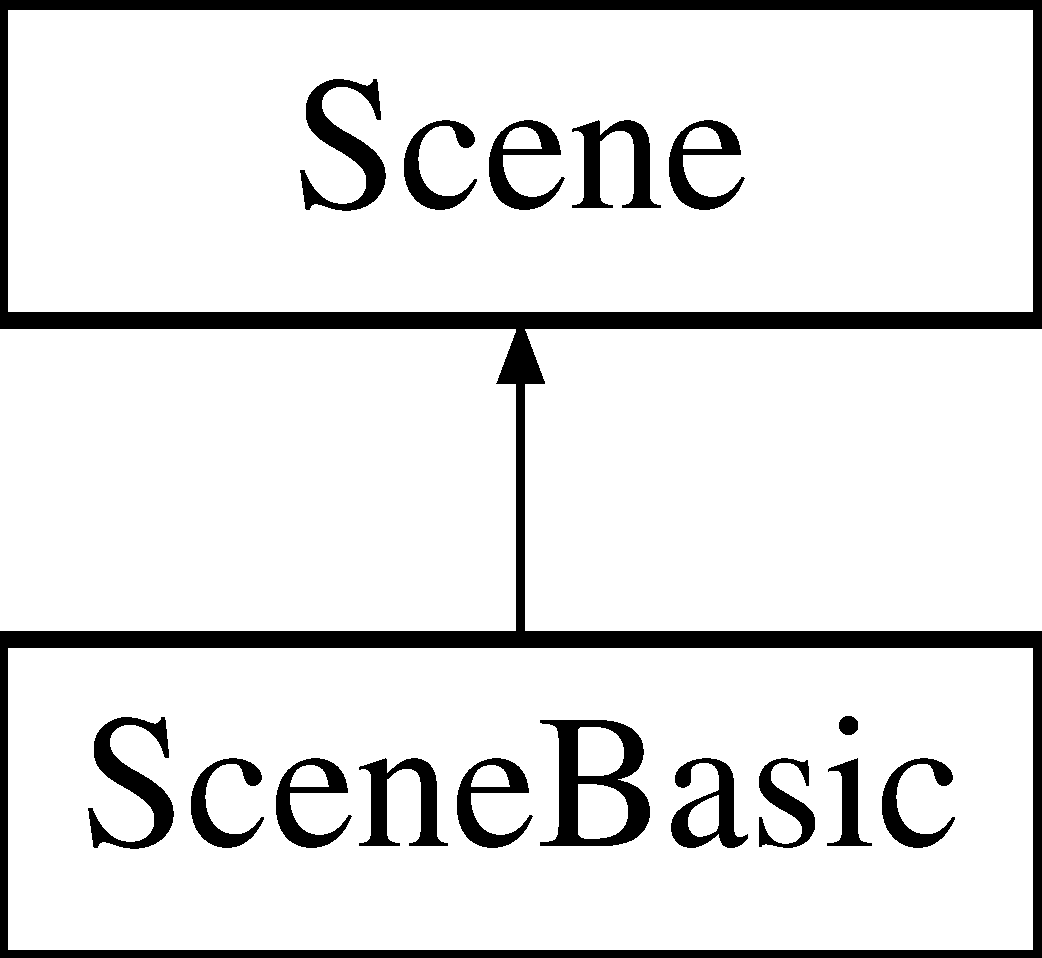
\includegraphics[height=2.000000cm]{class_scene_basic}
\end{center}
\end{figure}
\subsection*{Public Member Functions}
\begin{DoxyCompactItemize}
\item 
\hyperlink{class_scene_basic_a4eedd794e7e095992bda1566f2e3bd2e}{Scene\+Basic} ()
\begin{DoxyCompactList}\small\item\em Default constructor of \hyperlink{class_scene_basic}{Scene\+Basic}. \end{DoxyCompactList}\item 
std\+::vector$<$ double $>$ const  \& \hyperlink{class_scene_basic_ac805ba94deedc1f4d606d9554d088ea0}{get\+Center} ()
\begin{DoxyCompactList}\small\item\em Const Accessor inherited method wich provide the center of the cube. \end{DoxyCompactList}\item 
void \hyperlink{class_scene_basic_ac0cc945b040983d7527cda36963ec711}{Create\+V\+B\+O\+Line} ()
\begin{DoxyCompactList}\small\item\em Inherited function from scene. Create vbos for the line. \end{DoxyCompactList}\item 
void \hyperlink{class_scene_basic_a0575ddd74a9f9a5f238def19657f275e}{init\+Scene} ()
\begin{DoxyCompactList}\small\item\em Inherited function from scene. Initialize the scene. \end{DoxyCompactList}\item 
void \hyperlink{class_scene_basic_a8cfaad3ce6a4586e088b8d55d0e23ea6}{render} ()
\begin{DoxyCompactList}\small\item\em Inherited function from scene. Update the scene. \end{DoxyCompactList}\item 
void \hyperlink{class_scene_basic_af8a829370fa5e7386f46b5b659f3a083}{resize} (int, int)
\begin{DoxyCompactList}\small\item\em Resize the window. \end{DoxyCompactList}\item 
void \hyperlink{class_scene_basic_a40b11f479361056d418edbf0a14c9a59}{update} (float t)
\begin{DoxyCompactList}\small\item\em Update the angle. \end{DoxyCompactList}\item 
void \hyperlink{class_scene_basic_ae98490655b1c7cffe9ebeca001096b87}{set\+Angle\+Axis} (float ang, vec3 ax)
\begin{DoxyCompactList}\small\item\em Set the angle of the axis. \end{DoxyCompactList}\item 
void \hyperlink{class_scene_basic_abe43716a4f7a637850f725fcf14d4e5f}{print\+Active\+Uniforms} (G\+Luint program\+Handle)
\item 
void \hyperlink{class_scene_basic_a3a475225ffef7d3227401d762c7f2744}{print\+Active\+Attribs} (G\+Luint program\+Handle)
\item 
void \hyperlink{class_scene_basic_aa434179e3d31306f521f0d38c34baea3}{rotate\+Model} (\hyperlink{structset_of_values}{set\+Of\+Values} param)
\begin{DoxyCompactList}\small\item\em Do tranformations on the models. \end{DoxyCompactList}\item 
void \hyperlink{class_scene_basic_a3fa1c3ba519581687c7fe7214af8cc58}{update\+Eye\+Camera\+On\+Cube} (std\+::vector$<$ double $>$ center)
\begin{DoxyCompactList}\small\item\em Update the camera. \end{DoxyCompactList}\item 
void \hyperlink{class_scene_basic_abcd244d71f229f3d7c7133818c5e1898}{update\+Eye\+Camera\+User} (\hyperlink{structset_of_view}{set\+Of\+View} param)
\begin{DoxyCompactList}\small\item\em Set the camera with the parameters chosen by the user. \end{DoxyCompactList}\item 
void \hyperlink{class_scene_basic_ad7930ecd7654ac2c794ba666d71330e0}{restore\+Cam\+Default} ()
\begin{DoxyCompactList}\small\item\em Inherited function from scene. Restore the default parameters of the view and the cube. \end{DoxyCompactList}\end{DoxyCompactItemize}


\subsection{Detailed Description}
It is the scene of the project. Where all transformations, actions are done. 

\subsection{Constructor \& Destructor Documentation}
\hypertarget{class_scene_basic_a4eedd794e7e095992bda1566f2e3bd2e}{}\label{class_scene_basic_a4eedd794e7e095992bda1566f2e3bd2e} 
\index{Scene\+Basic@{Scene\+Basic}!Scene\+Basic@{Scene\+Basic}}
\index{Scene\+Basic@{Scene\+Basic}!Scene\+Basic@{Scene\+Basic}}
\subsubsection{\texorpdfstring{Scene\+Basic()}{SceneBasic()}}
{\footnotesize\ttfamily Scene\+Basic\+::\+Scene\+Basic (\begin{DoxyParamCaption}{ }\end{DoxyParamCaption})}



Default constructor of \hyperlink{class_scene_basic}{Scene\+Basic}. 



\subsection{Member Function Documentation}
\hypertarget{class_scene_basic_ac0cc945b040983d7527cda36963ec711}{}\label{class_scene_basic_ac0cc945b040983d7527cda36963ec711} 
\index{Scene\+Basic@{Scene\+Basic}!Create\+V\+B\+O\+Line@{Create\+V\+B\+O\+Line}}
\index{Create\+V\+B\+O\+Line@{Create\+V\+B\+O\+Line}!Scene\+Basic@{Scene\+Basic}}
\subsubsection{\texorpdfstring{Create\+V\+B\+O\+Line()}{CreateVBOLine()}}
{\footnotesize\ttfamily void Scene\+Basic\+::\+Create\+V\+B\+O\+Line (\begin{DoxyParamCaption}{ }\end{DoxyParamCaption})\hspace{0.3cm}{\ttfamily [virtual]}}



Inherited function from scene. Create vbos for the line. 



Implements \hyperlink{class_scene_a2e371aa848e8c30f593c2d9a2687dd28}{Scene}.

\hypertarget{class_scene_basic_ac805ba94deedc1f4d606d9554d088ea0}{}\label{class_scene_basic_ac805ba94deedc1f4d606d9554d088ea0} 
\index{Scene\+Basic@{Scene\+Basic}!get\+Center@{get\+Center}}
\index{get\+Center@{get\+Center}!Scene\+Basic@{Scene\+Basic}}
\subsubsection{\texorpdfstring{get\+Center()}{getCenter()}}
{\footnotesize\ttfamily std\+::vector$<$ double $>$ const  \& Scene\+Basic\+::get\+Center (\begin{DoxyParamCaption}{ }\end{DoxyParamCaption})\hspace{0.3cm}{\ttfamily [virtual]}}



Const Accessor inherited method wich provide the center of the cube. 

\begin{DoxyReturn}{Returns}
The center of the cube 
\end{DoxyReturn}


Implements \hyperlink{class_scene_a15d25044dbd65a8d7d0759888fcd55a1}{Scene}.

\hypertarget{class_scene_basic_a0575ddd74a9f9a5f238def19657f275e}{}\label{class_scene_basic_a0575ddd74a9f9a5f238def19657f275e} 
\index{Scene\+Basic@{Scene\+Basic}!init\+Scene@{init\+Scene}}
\index{init\+Scene@{init\+Scene}!Scene\+Basic@{Scene\+Basic}}
\subsubsection{\texorpdfstring{init\+Scene()}{initScene()}}
{\footnotesize\ttfamily void Scene\+Basic\+::init\+Scene (\begin{DoxyParamCaption}{ }\end{DoxyParamCaption})\hspace{0.3cm}{\ttfamily [virtual]}}



Inherited function from scene. Initialize the scene. 



Implements \hyperlink{class_scene_ae76b830c1156bb40bd744afb63776be2}{Scene}.

\hypertarget{class_scene_basic_a3a475225ffef7d3227401d762c7f2744}{}\label{class_scene_basic_a3a475225ffef7d3227401d762c7f2744} 
\index{Scene\+Basic@{Scene\+Basic}!print\+Active\+Attribs@{print\+Active\+Attribs}}
\index{print\+Active\+Attribs@{print\+Active\+Attribs}!Scene\+Basic@{Scene\+Basic}}
\subsubsection{\texorpdfstring{print\+Active\+Attribs()}{printActiveAttribs()}}
{\footnotesize\ttfamily void Scene\+Basic\+::print\+Active\+Attribs (\begin{DoxyParamCaption}\item[{G\+Luint}]{program\+Handle }\end{DoxyParamCaption})}

\hypertarget{class_scene_basic_abe43716a4f7a637850f725fcf14d4e5f}{}\label{class_scene_basic_abe43716a4f7a637850f725fcf14d4e5f} 
\index{Scene\+Basic@{Scene\+Basic}!print\+Active\+Uniforms@{print\+Active\+Uniforms}}
\index{print\+Active\+Uniforms@{print\+Active\+Uniforms}!Scene\+Basic@{Scene\+Basic}}
\subsubsection{\texorpdfstring{print\+Active\+Uniforms()}{printActiveUniforms()}}
{\footnotesize\ttfamily void Scene\+Basic\+::print\+Active\+Uniforms (\begin{DoxyParamCaption}\item[{G\+Luint}]{program\+Handle }\end{DoxyParamCaption})}

\hypertarget{class_scene_basic_a8cfaad3ce6a4586e088b8d55d0e23ea6}{}\label{class_scene_basic_a8cfaad3ce6a4586e088b8d55d0e23ea6} 
\index{Scene\+Basic@{Scene\+Basic}!render@{render}}
\index{render@{render}!Scene\+Basic@{Scene\+Basic}}
\subsubsection{\texorpdfstring{render()}{render()}}
{\footnotesize\ttfamily void Scene\+Basic\+::render (\begin{DoxyParamCaption}{ }\end{DoxyParamCaption})\hspace{0.3cm}{\ttfamily [virtual]}}



Inherited function from scene. Update the scene. 



Implements \hyperlink{class_scene_a823f4cd60d27932ee16f74adb0421ff6}{Scene}.

\hypertarget{class_scene_basic_af8a829370fa5e7386f46b5b659f3a083}{}\label{class_scene_basic_af8a829370fa5e7386f46b5b659f3a083} 
\index{Scene\+Basic@{Scene\+Basic}!resize@{resize}}
\index{resize@{resize}!Scene\+Basic@{Scene\+Basic}}
\subsubsection{\texorpdfstring{resize()}{resize()}}
{\footnotesize\ttfamily void Scene\+Basic\+::resize (\begin{DoxyParamCaption}\item[{int}]{w,  }\item[{int}]{h }\end{DoxyParamCaption})\hspace{0.3cm}{\ttfamily [virtual]}}



Resize the window. 



Implements \hyperlink{class_scene_a454bd0a09c125201fbb32e15d4f62fa3}{Scene}.

\hypertarget{class_scene_basic_ad7930ecd7654ac2c794ba666d71330e0}{}\label{class_scene_basic_ad7930ecd7654ac2c794ba666d71330e0} 
\index{Scene\+Basic@{Scene\+Basic}!restore\+Cam\+Default@{restore\+Cam\+Default}}
\index{restore\+Cam\+Default@{restore\+Cam\+Default}!Scene\+Basic@{Scene\+Basic}}
\subsubsection{\texorpdfstring{restore\+Cam\+Default()}{restoreCamDefault()}}
{\footnotesize\ttfamily void Scene\+Basic\+::restore\+Cam\+Default (\begin{DoxyParamCaption}{ }\end{DoxyParamCaption})\hspace{0.3cm}{\ttfamily [virtual]}}



Inherited function from scene. Restore the default parameters of the view and the cube. 



Implements \hyperlink{class_scene_a74dc104a3f44abf1f09d7b627c9baa36}{Scene}.

\hypertarget{class_scene_basic_aa434179e3d31306f521f0d38c34baea3}{}\label{class_scene_basic_aa434179e3d31306f521f0d38c34baea3} 
\index{Scene\+Basic@{Scene\+Basic}!rotate\+Model@{rotate\+Model}}
\index{rotate\+Model@{rotate\+Model}!Scene\+Basic@{Scene\+Basic}}
\subsubsection{\texorpdfstring{rotate\+Model()}{rotateModel()}}
{\footnotesize\ttfamily void Scene\+Basic\+::rotate\+Model (\begin{DoxyParamCaption}\item[{\hyperlink{structset_of_values}{set\+Of\+Values}}]{param }\end{DoxyParamCaption})\hspace{0.3cm}{\ttfamily [virtual]}}



Do tranformations on the models. 


\begin{DoxyParams}{Parameters}
{\em param} & set of values of the user when he choses the parameters of the line \\
\hline
\end{DoxyParams}


Implements \hyperlink{class_scene_af0c5ec79be9fbb4a6a2554ac4aaaf473}{Scene}.

\hypertarget{class_scene_basic_ae98490655b1c7cffe9ebeca001096b87}{}\label{class_scene_basic_ae98490655b1c7cffe9ebeca001096b87} 
\index{Scene\+Basic@{Scene\+Basic}!set\+Angle\+Axis@{set\+Angle\+Axis}}
\index{set\+Angle\+Axis@{set\+Angle\+Axis}!Scene\+Basic@{Scene\+Basic}}
\subsubsection{\texorpdfstring{set\+Angle\+Axis()}{setAngleAxis()}}
{\footnotesize\ttfamily void Scene\+Basic\+::set\+Angle\+Axis (\begin{DoxyParamCaption}\item[{float}]{ang,  }\item[{vec3}]{ax }\end{DoxyParamCaption})\hspace{0.3cm}{\ttfamily [virtual]}}



Set the angle of the axis. 


\begin{DoxyParams}{Parameters}
{\em ang} & angle \\
\hline
{\em ax} & axis \\
\hline
\end{DoxyParams}


Implements \hyperlink{class_scene_ab0c59864d813f7d11a2d362acfdd0e26}{Scene}.

\hypertarget{class_scene_basic_a40b11f479361056d418edbf0a14c9a59}{}\label{class_scene_basic_a40b11f479361056d418edbf0a14c9a59} 
\index{Scene\+Basic@{Scene\+Basic}!update@{update}}
\index{update@{update}!Scene\+Basic@{Scene\+Basic}}
\subsubsection{\texorpdfstring{update()}{update()}}
{\footnotesize\ttfamily void Scene\+Basic\+::update (\begin{DoxyParamCaption}\item[{float}]{t }\end{DoxyParamCaption})\hspace{0.3cm}{\ttfamily [virtual]}}



Update the angle. 


\begin{DoxyParams}{Parameters}
{\em t} & t$\ast$2$\ast$\+Pi$\ast$angle \\
\hline
\end{DoxyParams}


Implements \hyperlink{class_scene_aafa9ccf4d019005fdd41672afd13a7a9}{Scene}.

\hypertarget{class_scene_basic_a3fa1c3ba519581687c7fe7214af8cc58}{}\label{class_scene_basic_a3fa1c3ba519581687c7fe7214af8cc58} 
\index{Scene\+Basic@{Scene\+Basic}!update\+Eye\+Camera\+On\+Cube@{update\+Eye\+Camera\+On\+Cube}}
\index{update\+Eye\+Camera\+On\+Cube@{update\+Eye\+Camera\+On\+Cube}!Scene\+Basic@{Scene\+Basic}}
\subsubsection{\texorpdfstring{update\+Eye\+Camera\+On\+Cube()}{updateEyeCameraOnCube()}}
{\footnotesize\ttfamily void Scene\+Basic\+::update\+Eye\+Camera\+On\+Cube (\begin{DoxyParamCaption}\item[{std\+::vector$<$ double $>$}]{center }\end{DoxyParamCaption})\hspace{0.3cm}{\ttfamily [virtual]}}



Update the camera. 


\begin{DoxyParams}{Parameters}
{\em center} & center of the cube \\
\hline
\end{DoxyParams}


Implements \hyperlink{class_scene_a04ae3637cb26c4ad95004372d5a63654}{Scene}.

\hypertarget{class_scene_basic_abcd244d71f229f3d7c7133818c5e1898}{}\label{class_scene_basic_abcd244d71f229f3d7c7133818c5e1898} 
\index{Scene\+Basic@{Scene\+Basic}!update\+Eye\+Camera\+User@{update\+Eye\+Camera\+User}}
\index{update\+Eye\+Camera\+User@{update\+Eye\+Camera\+User}!Scene\+Basic@{Scene\+Basic}}
\subsubsection{\texorpdfstring{update\+Eye\+Camera\+User()}{updateEyeCameraUser()}}
{\footnotesize\ttfamily void Scene\+Basic\+::update\+Eye\+Camera\+User (\begin{DoxyParamCaption}\item[{\hyperlink{structset_of_view}{set\+Of\+View}}]{param }\end{DoxyParamCaption})\hspace{0.3cm}{\ttfamily [virtual]}}



Set the camera with the parameters chosen by the user. 


\begin{DoxyParams}{Parameters}
{\em param} & set of values of the user when he choses the parameters of the camera \\
\hline
\end{DoxyParams}


Implements \hyperlink{class_scene_a52181459b75a0c2f4706a26f3e200ca1}{Scene}.



The documentation for this class was generated from the following files\+:\begin{DoxyCompactItemize}
\item 
D\+:/\+Q\+T\+\_\+projets/\+Cube\+Menu/\hyperlink{scenebasic_8h}{scenebasic.\+h}\item 
D\+:/\+Q\+T\+\_\+projets/\+Cube\+Menu/\hyperlink{scenebasic_8cpp}{scenebasic.\+cpp}\end{DoxyCompactItemize}

\hypertarget{struct_set_of_values}{}\section{Set\+Of\+Values Struct Reference}
\label{struct_set_of_values}\index{Set\+Of\+Values@{Set\+Of\+Values}}


{\ttfamily \#include \char`\"{}Parameters of the G\+U\+I of the line\char`\"{}}



\subsection{Detailed Description}


The documentation for this struct was generated from the following file\+:\begin{DoxyCompactItemize}
\item 
D\+:/\+Q\+T\+\_\+projets/\+Cube\+Menu/\hyperlink{dialog_8h}{dialog.\+h}\end{DoxyCompactItemize}

\hypertarget{structset_of_values}{}\section{set\+Of\+Values Struct Reference}
\label{structset_of_values}\index{set\+Of\+Values@{set\+Of\+Values}}


{\ttfamily \#include $<$dialog.\+h$>$}

\subsection*{Public Attributes}
\begin{DoxyCompactItemize}
\item 
double \hyperlink{structset_of_values_af51a2722732fb80f626e6ab9c1f1fed3}{xB}
\item 
double \hyperlink{structset_of_values_a64756693023b45c80cbb542fd2f834e3}{yB}
\item 
double \hyperlink{structset_of_values_a00e8dca4650208fa2d9a7c8cce72bae2}{zB}
\item 
double \hyperlink{structset_of_values_ab937d8ca1493a6b7fcb4ec13a6507dd1}{xD}
\item 
double \hyperlink{structset_of_values_a229a82279aeb68d2b63c3ca81d12a4db}{yD}
\item 
double \hyperlink{structset_of_values_ae75c3668aeac869d48699ce68ab58375}{zD}
\item 
double \hyperlink{structset_of_values_a80a95f64eeeaf8e9fd70be85f6a47a77}{alpha}
\end{DoxyCompactItemize}


\subsection{Member Data Documentation}
\hypertarget{structset_of_values_a80a95f64eeeaf8e9fd70be85f6a47a77}{}\label{structset_of_values_a80a95f64eeeaf8e9fd70be85f6a47a77} 
\index{set\+Of\+Values@{set\+Of\+Values}!alpha@{alpha}}
\index{alpha@{alpha}!set\+Of\+Values@{set\+Of\+Values}}
\subsubsection{\texorpdfstring{alpha}{alpha}}
{\footnotesize\ttfamily double set\+Of\+Values\+::alpha}

\hypertarget{structset_of_values_af51a2722732fb80f626e6ab9c1f1fed3}{}\label{structset_of_values_af51a2722732fb80f626e6ab9c1f1fed3} 
\index{set\+Of\+Values@{set\+Of\+Values}!xB@{xB}}
\index{xB@{xB}!set\+Of\+Values@{set\+Of\+Values}}
\subsubsection{\texorpdfstring{xB}{xB}}
{\footnotesize\ttfamily double set\+Of\+Values\+::xB}

\hypertarget{structset_of_values_ab937d8ca1493a6b7fcb4ec13a6507dd1}{}\label{structset_of_values_ab937d8ca1493a6b7fcb4ec13a6507dd1} 
\index{set\+Of\+Values@{set\+Of\+Values}!xD@{xD}}
\index{xD@{xD}!set\+Of\+Values@{set\+Of\+Values}}
\subsubsection{\texorpdfstring{xD}{xD}}
{\footnotesize\ttfamily double set\+Of\+Values\+::xD}

\hypertarget{structset_of_values_a64756693023b45c80cbb542fd2f834e3}{}\label{structset_of_values_a64756693023b45c80cbb542fd2f834e3} 
\index{set\+Of\+Values@{set\+Of\+Values}!yB@{yB}}
\index{yB@{yB}!set\+Of\+Values@{set\+Of\+Values}}
\subsubsection{\texorpdfstring{yB}{yB}}
{\footnotesize\ttfamily double set\+Of\+Values\+::yB}

\hypertarget{structset_of_values_a229a82279aeb68d2b63c3ca81d12a4db}{}\label{structset_of_values_a229a82279aeb68d2b63c3ca81d12a4db} 
\index{set\+Of\+Values@{set\+Of\+Values}!yD@{yD}}
\index{yD@{yD}!set\+Of\+Values@{set\+Of\+Values}}
\subsubsection{\texorpdfstring{yD}{yD}}
{\footnotesize\ttfamily double set\+Of\+Values\+::yD}

\hypertarget{structset_of_values_a00e8dca4650208fa2d9a7c8cce72bae2}{}\label{structset_of_values_a00e8dca4650208fa2d9a7c8cce72bae2} 
\index{set\+Of\+Values@{set\+Of\+Values}!zB@{zB}}
\index{zB@{zB}!set\+Of\+Values@{set\+Of\+Values}}
\subsubsection{\texorpdfstring{zB}{zB}}
{\footnotesize\ttfamily double set\+Of\+Values\+::zB}

\hypertarget{structset_of_values_ae75c3668aeac869d48699ce68ab58375}{}\label{structset_of_values_ae75c3668aeac869d48699ce68ab58375} 
\index{set\+Of\+Values@{set\+Of\+Values}!zD@{zD}}
\index{zD@{zD}!set\+Of\+Values@{set\+Of\+Values}}
\subsubsection{\texorpdfstring{zD}{zD}}
{\footnotesize\ttfamily double set\+Of\+Values\+::zD}



The documentation for this struct was generated from the following file\+:\begin{DoxyCompactItemize}
\item 
D\+:/\+Q\+T\+\_\+projets/\+Cube\+Menu/\hyperlink{dialog_8h}{dialog.\+h}\end{DoxyCompactItemize}

\hypertarget{struct_set_of_view}{}\section{Set\+Of\+View Struct Reference}
\label{struct_set_of_view}\index{Set\+Of\+View@{Set\+Of\+View}}


{\ttfamily \#include \char`\"{}Parameters of the G\+U\+I of the camera\char`\"{}}



\subsection{Detailed Description}


The documentation for this struct was generated from the following file\+:\begin{DoxyCompactItemize}
\item 
D\+:/\+Q\+T\+\_\+projets/\+Cube\+Menu/\hyperlink{dialogeyes_8h}{dialogeyes.\+h}\end{DoxyCompactItemize}

\hypertarget{structset_of_view}{}\section{set\+Of\+View Struct Reference}
\label{structset_of_view}\index{set\+Of\+View@{set\+Of\+View}}


{\ttfamily \#include $<$dialogeyes.\+h$>$}

\subsection*{Public Attributes}
\begin{DoxyCompactItemize}
\item 
double \hyperlink{structset_of_view_a0bb9d7f541ae499a85494ccb697e48fc}{eyex}
\item 
double \hyperlink{structset_of_view_af7c9b4ac6d7a4098d3b4639b2763376e}{eyey}
\item 
double \hyperlink{structset_of_view_ae8bf003e65ba68562d248ade07168b8e}{eyez}
\item 
double \hyperlink{structset_of_view_a91713a1fe5754075293a26ff11cbc5fb}{directx}
\item 
double \hyperlink{structset_of_view_a3edfcb674ff889fa9779ff9483ccdd5e}{directy}
\item 
double \hyperlink{structset_of_view_a6c47319cf5b1aadaacb5fbbcdc4ab280}{directz}
\end{DoxyCompactItemize}


\subsection{Member Data Documentation}
\hypertarget{structset_of_view_a91713a1fe5754075293a26ff11cbc5fb}{}\label{structset_of_view_a91713a1fe5754075293a26ff11cbc5fb} 
\index{set\+Of\+View@{set\+Of\+View}!directx@{directx}}
\index{directx@{directx}!set\+Of\+View@{set\+Of\+View}}
\subsubsection{\texorpdfstring{directx}{directx}}
{\footnotesize\ttfamily double set\+Of\+View\+::directx}

\hypertarget{structset_of_view_a3edfcb674ff889fa9779ff9483ccdd5e}{}\label{structset_of_view_a3edfcb674ff889fa9779ff9483ccdd5e} 
\index{set\+Of\+View@{set\+Of\+View}!directy@{directy}}
\index{directy@{directy}!set\+Of\+View@{set\+Of\+View}}
\subsubsection{\texorpdfstring{directy}{directy}}
{\footnotesize\ttfamily double set\+Of\+View\+::directy}

\hypertarget{structset_of_view_a6c47319cf5b1aadaacb5fbbcdc4ab280}{}\label{structset_of_view_a6c47319cf5b1aadaacb5fbbcdc4ab280} 
\index{set\+Of\+View@{set\+Of\+View}!directz@{directz}}
\index{directz@{directz}!set\+Of\+View@{set\+Of\+View}}
\subsubsection{\texorpdfstring{directz}{directz}}
{\footnotesize\ttfamily double set\+Of\+View\+::directz}

\hypertarget{structset_of_view_a0bb9d7f541ae499a85494ccb697e48fc}{}\label{structset_of_view_a0bb9d7f541ae499a85494ccb697e48fc} 
\index{set\+Of\+View@{set\+Of\+View}!eyex@{eyex}}
\index{eyex@{eyex}!set\+Of\+View@{set\+Of\+View}}
\subsubsection{\texorpdfstring{eyex}{eyex}}
{\footnotesize\ttfamily double set\+Of\+View\+::eyex}

\hypertarget{structset_of_view_af7c9b4ac6d7a4098d3b4639b2763376e}{}\label{structset_of_view_af7c9b4ac6d7a4098d3b4639b2763376e} 
\index{set\+Of\+View@{set\+Of\+View}!eyey@{eyey}}
\index{eyey@{eyey}!set\+Of\+View@{set\+Of\+View}}
\subsubsection{\texorpdfstring{eyey}{eyey}}
{\footnotesize\ttfamily double set\+Of\+View\+::eyey}

\hypertarget{structset_of_view_ae8bf003e65ba68562d248ade07168b8e}{}\label{structset_of_view_ae8bf003e65ba68562d248ade07168b8e} 
\index{set\+Of\+View@{set\+Of\+View}!eyez@{eyez}}
\index{eyez@{eyez}!set\+Of\+View@{set\+Of\+View}}
\subsubsection{\texorpdfstring{eyez}{eyez}}
{\footnotesize\ttfamily double set\+Of\+View\+::eyez}



The documentation for this struct was generated from the following file\+:\begin{DoxyCompactItemize}
\item 
D\+:/\+Q\+T\+\_\+projets/\+Cube\+Menu/\hyperlink{dialogeyes_8h}{dialogeyes.\+h}\end{DoxyCompactItemize}

\hypertarget{class_ui___dialog}{}\section{Ui\+\_\+\+Dialog Class Reference}
\label{class_ui___dialog}\index{Ui\+\_\+\+Dialog@{Ui\+\_\+\+Dialog}}


{\ttfamily \#include $<$ui\+\_\+dialog.\+h$>$}

Inheritance diagram for Ui\+\_\+\+Dialog\+:\begin{figure}[H]
\begin{center}
\leavevmode
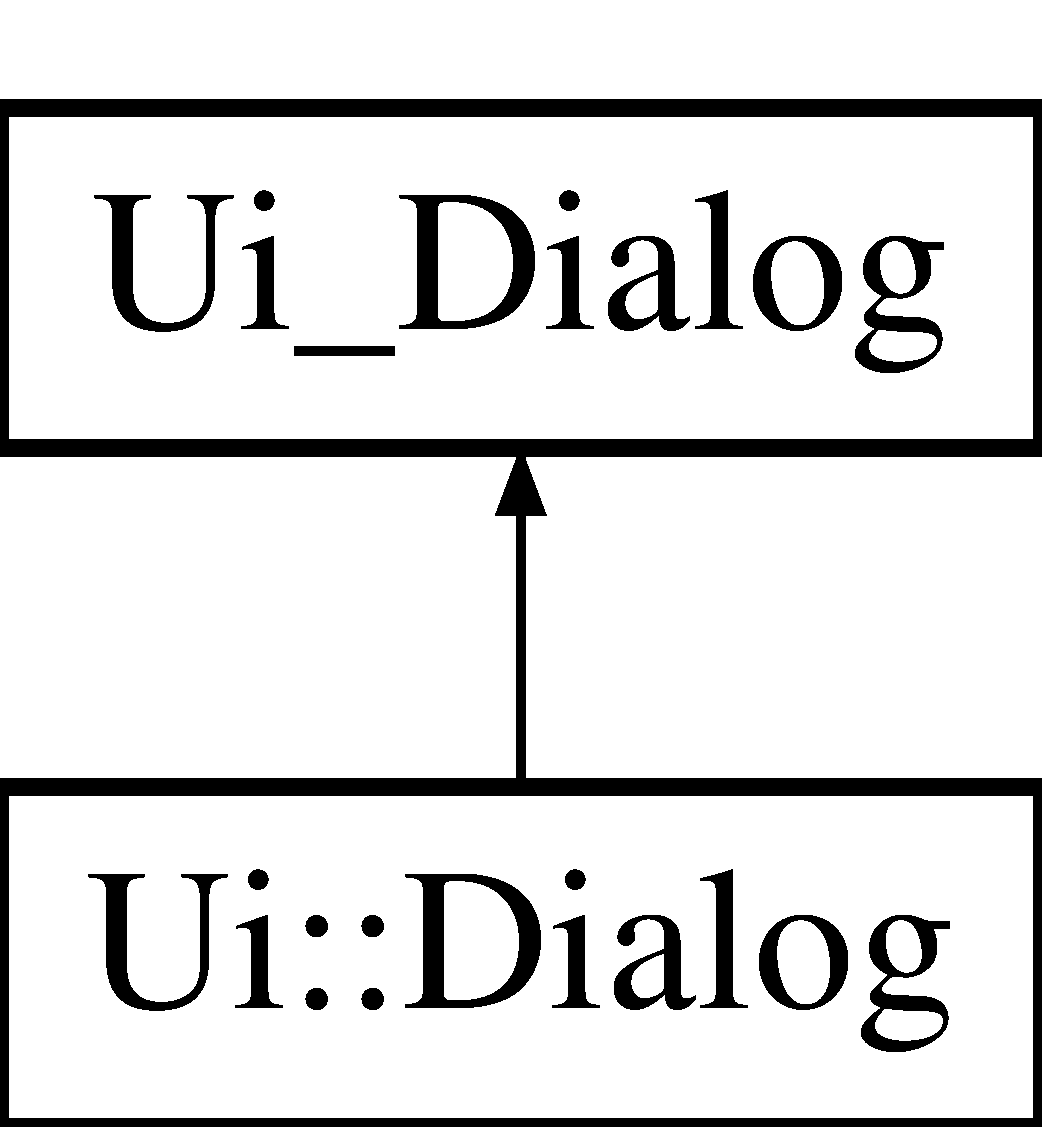
\includegraphics[height=2.000000cm]{class_ui___dialog}
\end{center}
\end{figure}
\subsection*{Public Member Functions}
\begin{DoxyCompactItemize}
\item 
void \hyperlink{class_ui___dialog_a4f6a478c3ecdafabffb17b39cb26444a}{setup\+Ui} (Q\+Dialog $\ast$\hyperlink{class_dialog}{Dialog})
\item 
void \hyperlink{class_ui___dialog_afa0ccb6f716ca6178260522a193c250e}{retranslate\+Ui} (Q\+Dialog $\ast$\hyperlink{class_dialog}{Dialog})
\end{DoxyCompactItemize}
\subsection*{Public Attributes}
\begin{DoxyCompactItemize}
\item 
Q\+Widget $\ast$ \hyperlink{class_ui___dialog_af56f0c59b650c50a635d4b11890c172e}{grid\+Layout\+Widget}
\item 
Q\+Grid\+Layout $\ast$ \hyperlink{class_ui___dialog_a41336d41594e8776a81d095e8e4ffc61}{grid\+Layout}
\item 
Q\+V\+Box\+Layout $\ast$ \hyperlink{class_ui___dialog_acd165ec013acc890cb290ce16b9563f6}{vertical\+Layout\+\_\+3}
\item 
Q\+Label $\ast$ \hyperlink{class_ui___dialog_aa90f8f5a9ff9c2260913ff6c04e18702}{label\+\_\+chooseD}
\item 
Q\+Grid\+Layout $\ast$ \hyperlink{class_ui___dialog_a95e4393e872e5101ebfc05e5e5cd182f}{grid\+Layout\+\_\+3}
\item 
Q\+Double\+Spin\+Box $\ast$ \hyperlink{class_ui___dialog_af56082e875190dce33551c7b80637f67}{double\+Spin\+Box\+\_\+z\+\_\+d}
\item 
Q\+Double\+Spin\+Box $\ast$ \hyperlink{class_ui___dialog_a979c774889164d711599270126aa7f7a}{double\+Spin\+Box\+\_\+x\+\_\+d}
\item 
Q\+Label $\ast$ \hyperlink{class_ui___dialog_a6dfc56c2ed0c6f1141dddb9ce6ce65f7}{label\+\_\+y\+\_\+d}
\item 
Q\+Label $\ast$ \hyperlink{class_ui___dialog_a24bc1d94076a61c599e0626cce0ecbff}{label\+\_\+x\+\_\+d}
\item 
Q\+Label $\ast$ \hyperlink{class_ui___dialog_a680efd605623366cfbd396c56bfe8fbd}{label\+\_\+z\+\_\+d}
\item 
Q\+Double\+Spin\+Box $\ast$ \hyperlink{class_ui___dialog_a81747c4db62ac24a132abe8cf5270405}{double\+Spin\+Box\+\_\+y\+\_\+d}
\item 
Q\+V\+Box\+Layout $\ast$ \hyperlink{class_ui___dialog_a4fb6d1c8d4780f0d513f4a48af4a2b10}{vertical\+Layout\+\_\+2}
\item 
Q\+Label $\ast$ \hyperlink{class_ui___dialog_afdb95c03e64a971906bad7a49fbb887f}{label\+\_\+equation\+\_\+general}
\item 
Q\+Label $\ast$ \hyperlink{class_ui___dialog_a71bdeed53adf9ef8db30eb55a879864a}{label\+\_\+choose\+B\+\_\+2}
\item 
Q\+Grid\+Layout $\ast$ \hyperlink{class_ui___dialog_af3de0f6556fd8c9d0aac09a2f90d92b9}{grid\+Layout\+\_\+2}
\item 
Q\+Double\+Spin\+Box $\ast$ \hyperlink{class_ui___dialog_acb6d62af6a65734d26b419c39fac30bd}{double\+Spin\+Box\+\_\+x\+\_\+b}
\item 
Q\+Double\+Spin\+Box $\ast$ \hyperlink{class_ui___dialog_a20dc0d9e1d1c6829f8c1969bc1bfc6c8}{double\+Spin\+Box\+\_\+z\+\_\+b}
\item 
Q\+Label $\ast$ \hyperlink{class_ui___dialog_a0fced57090e5ac447ac60756bc36a68d}{label\+\_\+y\+\_\+b\+\_\+2}
\item 
Q\+Label $\ast$ \hyperlink{class_ui___dialog_a60553ee369483b9b346c5ad7377765e2}{label\+\_\+x\+\_\+b\+\_\+2}
\item 
Q\+Label $\ast$ \hyperlink{class_ui___dialog_a6ca6cabd6bb980d5804d866d1c166dd7}{label\+\_\+z\+\_\+b\+\_\+2}
\item 
Q\+Double\+Spin\+Box $\ast$ \hyperlink{class_ui___dialog_aa3d1e02dcb0016a94ac9810fff2c55f4}{double\+Spin\+Box\+\_\+y\+\_\+b}
\item 
Q\+V\+Box\+Layout $\ast$ \hyperlink{class_ui___dialog_a02f973813b741621c5461918b3d9d4bb}{vertical\+Layout}
\item 
Q\+V\+Box\+Layout $\ast$ \hyperlink{class_ui___dialog_a5ea05598d639698eabf0cbc00b1f0180}{vertical\+Layout\+\_\+4}
\item 
Q\+Label $\ast$ \hyperlink{class_ui___dialog_ac3844fd0281707dc5535826da7506ca5}{label}
\item 
Q\+Double\+Spin\+Box $\ast$ \hyperlink{class_ui___dialog_a45223f3641a2da220e880eba8c7ae100}{double\+Spin\+Box\+\_\+value\+\_\+alpha}
\item 
Q\+Dialog\+Button\+Box $\ast$ \hyperlink{class_ui___dialog_a271a59402f80983c2722bb455db37365}{button\+Box}
\item 
Q\+Push\+Button $\ast$ \hyperlink{class_ui___dialog_aebeace7895da27076f8f90c301742ec3}{push\+Button}
\end{DoxyCompactItemize}


\subsection{Member Function Documentation}
\hypertarget{class_ui___dialog_afa0ccb6f716ca6178260522a193c250e}{}\label{class_ui___dialog_afa0ccb6f716ca6178260522a193c250e} 
\index{Ui\+\_\+\+Dialog@{Ui\+\_\+\+Dialog}!retranslate\+Ui@{retranslate\+Ui}}
\index{retranslate\+Ui@{retranslate\+Ui}!Ui\+\_\+\+Dialog@{Ui\+\_\+\+Dialog}}
\subsubsection{\texorpdfstring{retranslate\+Ui()}{retranslateUi()}}
{\footnotesize\ttfamily void Ui\+\_\+\+Dialog\+::retranslate\+Ui (\begin{DoxyParamCaption}\item[{Q\+Dialog $\ast$}]{Dialog }\end{DoxyParamCaption})\hspace{0.3cm}{\ttfamily [inline]}}

\hypertarget{class_ui___dialog_a4f6a478c3ecdafabffb17b39cb26444a}{}\label{class_ui___dialog_a4f6a478c3ecdafabffb17b39cb26444a} 
\index{Ui\+\_\+\+Dialog@{Ui\+\_\+\+Dialog}!setup\+Ui@{setup\+Ui}}
\index{setup\+Ui@{setup\+Ui}!Ui\+\_\+\+Dialog@{Ui\+\_\+\+Dialog}}
\subsubsection{\texorpdfstring{setup\+Ui()}{setupUi()}}
{\footnotesize\ttfamily void Ui\+\_\+\+Dialog\+::setup\+Ui (\begin{DoxyParamCaption}\item[{Q\+Dialog $\ast$}]{Dialog }\end{DoxyParamCaption})\hspace{0.3cm}{\ttfamily [inline]}}



\subsection{Member Data Documentation}
\hypertarget{class_ui___dialog_a271a59402f80983c2722bb455db37365}{}\label{class_ui___dialog_a271a59402f80983c2722bb455db37365} 
\index{Ui\+\_\+\+Dialog@{Ui\+\_\+\+Dialog}!button\+Box@{button\+Box}}
\index{button\+Box@{button\+Box}!Ui\+\_\+\+Dialog@{Ui\+\_\+\+Dialog}}
\subsubsection{\texorpdfstring{button\+Box}{buttonBox}}
{\footnotesize\ttfamily Q\+Dialog\+Button\+Box$\ast$ Ui\+\_\+\+Dialog\+::button\+Box}

\hypertarget{class_ui___dialog_a45223f3641a2da220e880eba8c7ae100}{}\label{class_ui___dialog_a45223f3641a2da220e880eba8c7ae100} 
\index{Ui\+\_\+\+Dialog@{Ui\+\_\+\+Dialog}!double\+Spin\+Box\+\_\+value\+\_\+alpha@{double\+Spin\+Box\+\_\+value\+\_\+alpha}}
\index{double\+Spin\+Box\+\_\+value\+\_\+alpha@{double\+Spin\+Box\+\_\+value\+\_\+alpha}!Ui\+\_\+\+Dialog@{Ui\+\_\+\+Dialog}}
\subsubsection{\texorpdfstring{double\+Spin\+Box\+\_\+value\+\_\+alpha}{doubleSpinBox\_value\_alpha}}
{\footnotesize\ttfamily Q\+Double\+Spin\+Box$\ast$ Ui\+\_\+\+Dialog\+::double\+Spin\+Box\+\_\+value\+\_\+alpha}

\hypertarget{class_ui___dialog_acb6d62af6a65734d26b419c39fac30bd}{}\label{class_ui___dialog_acb6d62af6a65734d26b419c39fac30bd} 
\index{Ui\+\_\+\+Dialog@{Ui\+\_\+\+Dialog}!double\+Spin\+Box\+\_\+x\+\_\+b@{double\+Spin\+Box\+\_\+x\+\_\+b}}
\index{double\+Spin\+Box\+\_\+x\+\_\+b@{double\+Spin\+Box\+\_\+x\+\_\+b}!Ui\+\_\+\+Dialog@{Ui\+\_\+\+Dialog}}
\subsubsection{\texorpdfstring{double\+Spin\+Box\+\_\+x\+\_\+b}{doubleSpinBox\_x\_b}}
{\footnotesize\ttfamily Q\+Double\+Spin\+Box$\ast$ Ui\+\_\+\+Dialog\+::double\+Spin\+Box\+\_\+x\+\_\+b}

\hypertarget{class_ui___dialog_a979c774889164d711599270126aa7f7a}{}\label{class_ui___dialog_a979c774889164d711599270126aa7f7a} 
\index{Ui\+\_\+\+Dialog@{Ui\+\_\+\+Dialog}!double\+Spin\+Box\+\_\+x\+\_\+d@{double\+Spin\+Box\+\_\+x\+\_\+d}}
\index{double\+Spin\+Box\+\_\+x\+\_\+d@{double\+Spin\+Box\+\_\+x\+\_\+d}!Ui\+\_\+\+Dialog@{Ui\+\_\+\+Dialog}}
\subsubsection{\texorpdfstring{double\+Spin\+Box\+\_\+x\+\_\+d}{doubleSpinBox\_x\_d}}
{\footnotesize\ttfamily Q\+Double\+Spin\+Box$\ast$ Ui\+\_\+\+Dialog\+::double\+Spin\+Box\+\_\+x\+\_\+d}

\hypertarget{class_ui___dialog_aa3d1e02dcb0016a94ac9810fff2c55f4}{}\label{class_ui___dialog_aa3d1e02dcb0016a94ac9810fff2c55f4} 
\index{Ui\+\_\+\+Dialog@{Ui\+\_\+\+Dialog}!double\+Spin\+Box\+\_\+y\+\_\+b@{double\+Spin\+Box\+\_\+y\+\_\+b}}
\index{double\+Spin\+Box\+\_\+y\+\_\+b@{double\+Spin\+Box\+\_\+y\+\_\+b}!Ui\+\_\+\+Dialog@{Ui\+\_\+\+Dialog}}
\subsubsection{\texorpdfstring{double\+Spin\+Box\+\_\+y\+\_\+b}{doubleSpinBox\_y\_b}}
{\footnotesize\ttfamily Q\+Double\+Spin\+Box$\ast$ Ui\+\_\+\+Dialog\+::double\+Spin\+Box\+\_\+y\+\_\+b}

\hypertarget{class_ui___dialog_a81747c4db62ac24a132abe8cf5270405}{}\label{class_ui___dialog_a81747c4db62ac24a132abe8cf5270405} 
\index{Ui\+\_\+\+Dialog@{Ui\+\_\+\+Dialog}!double\+Spin\+Box\+\_\+y\+\_\+d@{double\+Spin\+Box\+\_\+y\+\_\+d}}
\index{double\+Spin\+Box\+\_\+y\+\_\+d@{double\+Spin\+Box\+\_\+y\+\_\+d}!Ui\+\_\+\+Dialog@{Ui\+\_\+\+Dialog}}
\subsubsection{\texorpdfstring{double\+Spin\+Box\+\_\+y\+\_\+d}{doubleSpinBox\_y\_d}}
{\footnotesize\ttfamily Q\+Double\+Spin\+Box$\ast$ Ui\+\_\+\+Dialog\+::double\+Spin\+Box\+\_\+y\+\_\+d}

\hypertarget{class_ui___dialog_a20dc0d9e1d1c6829f8c1969bc1bfc6c8}{}\label{class_ui___dialog_a20dc0d9e1d1c6829f8c1969bc1bfc6c8} 
\index{Ui\+\_\+\+Dialog@{Ui\+\_\+\+Dialog}!double\+Spin\+Box\+\_\+z\+\_\+b@{double\+Spin\+Box\+\_\+z\+\_\+b}}
\index{double\+Spin\+Box\+\_\+z\+\_\+b@{double\+Spin\+Box\+\_\+z\+\_\+b}!Ui\+\_\+\+Dialog@{Ui\+\_\+\+Dialog}}
\subsubsection{\texorpdfstring{double\+Spin\+Box\+\_\+z\+\_\+b}{doubleSpinBox\_z\_b}}
{\footnotesize\ttfamily Q\+Double\+Spin\+Box$\ast$ Ui\+\_\+\+Dialog\+::double\+Spin\+Box\+\_\+z\+\_\+b}

\hypertarget{class_ui___dialog_af56082e875190dce33551c7b80637f67}{}\label{class_ui___dialog_af56082e875190dce33551c7b80637f67} 
\index{Ui\+\_\+\+Dialog@{Ui\+\_\+\+Dialog}!double\+Spin\+Box\+\_\+z\+\_\+d@{double\+Spin\+Box\+\_\+z\+\_\+d}}
\index{double\+Spin\+Box\+\_\+z\+\_\+d@{double\+Spin\+Box\+\_\+z\+\_\+d}!Ui\+\_\+\+Dialog@{Ui\+\_\+\+Dialog}}
\subsubsection{\texorpdfstring{double\+Spin\+Box\+\_\+z\+\_\+d}{doubleSpinBox\_z\_d}}
{\footnotesize\ttfamily Q\+Double\+Spin\+Box$\ast$ Ui\+\_\+\+Dialog\+::double\+Spin\+Box\+\_\+z\+\_\+d}

\hypertarget{class_ui___dialog_a41336d41594e8776a81d095e8e4ffc61}{}\label{class_ui___dialog_a41336d41594e8776a81d095e8e4ffc61} 
\index{Ui\+\_\+\+Dialog@{Ui\+\_\+\+Dialog}!grid\+Layout@{grid\+Layout}}
\index{grid\+Layout@{grid\+Layout}!Ui\+\_\+\+Dialog@{Ui\+\_\+\+Dialog}}
\subsubsection{\texorpdfstring{grid\+Layout}{gridLayout}}
{\footnotesize\ttfamily Q\+Grid\+Layout$\ast$ Ui\+\_\+\+Dialog\+::grid\+Layout}

\hypertarget{class_ui___dialog_af3de0f6556fd8c9d0aac09a2f90d92b9}{}\label{class_ui___dialog_af3de0f6556fd8c9d0aac09a2f90d92b9} 
\index{Ui\+\_\+\+Dialog@{Ui\+\_\+\+Dialog}!grid\+Layout\+\_\+2@{grid\+Layout\+\_\+2}}
\index{grid\+Layout\+\_\+2@{grid\+Layout\+\_\+2}!Ui\+\_\+\+Dialog@{Ui\+\_\+\+Dialog}}
\subsubsection{\texorpdfstring{grid\+Layout\+\_\+2}{gridLayout\_2}}
{\footnotesize\ttfamily Q\+Grid\+Layout$\ast$ Ui\+\_\+\+Dialog\+::grid\+Layout\+\_\+2}

\hypertarget{class_ui___dialog_a95e4393e872e5101ebfc05e5e5cd182f}{}\label{class_ui___dialog_a95e4393e872e5101ebfc05e5e5cd182f} 
\index{Ui\+\_\+\+Dialog@{Ui\+\_\+\+Dialog}!grid\+Layout\+\_\+3@{grid\+Layout\+\_\+3}}
\index{grid\+Layout\+\_\+3@{grid\+Layout\+\_\+3}!Ui\+\_\+\+Dialog@{Ui\+\_\+\+Dialog}}
\subsubsection{\texorpdfstring{grid\+Layout\+\_\+3}{gridLayout\_3}}
{\footnotesize\ttfamily Q\+Grid\+Layout$\ast$ Ui\+\_\+\+Dialog\+::grid\+Layout\+\_\+3}

\hypertarget{class_ui___dialog_af56f0c59b650c50a635d4b11890c172e}{}\label{class_ui___dialog_af56f0c59b650c50a635d4b11890c172e} 
\index{Ui\+\_\+\+Dialog@{Ui\+\_\+\+Dialog}!grid\+Layout\+Widget@{grid\+Layout\+Widget}}
\index{grid\+Layout\+Widget@{grid\+Layout\+Widget}!Ui\+\_\+\+Dialog@{Ui\+\_\+\+Dialog}}
\subsubsection{\texorpdfstring{grid\+Layout\+Widget}{gridLayoutWidget}}
{\footnotesize\ttfamily Q\+Widget$\ast$ Ui\+\_\+\+Dialog\+::grid\+Layout\+Widget}

\hypertarget{class_ui___dialog_ac3844fd0281707dc5535826da7506ca5}{}\label{class_ui___dialog_ac3844fd0281707dc5535826da7506ca5} 
\index{Ui\+\_\+\+Dialog@{Ui\+\_\+\+Dialog}!label@{label}}
\index{label@{label}!Ui\+\_\+\+Dialog@{Ui\+\_\+\+Dialog}}
\subsubsection{\texorpdfstring{label}{label}}
{\footnotesize\ttfamily Q\+Label$\ast$ Ui\+\_\+\+Dialog\+::label}

\hypertarget{class_ui___dialog_a71bdeed53adf9ef8db30eb55a879864a}{}\label{class_ui___dialog_a71bdeed53adf9ef8db30eb55a879864a} 
\index{Ui\+\_\+\+Dialog@{Ui\+\_\+\+Dialog}!label\+\_\+choose\+B\+\_\+2@{label\+\_\+choose\+B\+\_\+2}}
\index{label\+\_\+choose\+B\+\_\+2@{label\+\_\+choose\+B\+\_\+2}!Ui\+\_\+\+Dialog@{Ui\+\_\+\+Dialog}}
\subsubsection{\texorpdfstring{label\+\_\+choose\+B\+\_\+2}{label\_chooseB\_2}}
{\footnotesize\ttfamily Q\+Label$\ast$ Ui\+\_\+\+Dialog\+::label\+\_\+choose\+B\+\_\+2}

\hypertarget{class_ui___dialog_aa90f8f5a9ff9c2260913ff6c04e18702}{}\label{class_ui___dialog_aa90f8f5a9ff9c2260913ff6c04e18702} 
\index{Ui\+\_\+\+Dialog@{Ui\+\_\+\+Dialog}!label\+\_\+chooseD@{label\+\_\+chooseD}}
\index{label\+\_\+chooseD@{label\+\_\+chooseD}!Ui\+\_\+\+Dialog@{Ui\+\_\+\+Dialog}}
\subsubsection{\texorpdfstring{label\+\_\+chooseD}{label\_chooseD}}
{\footnotesize\ttfamily Q\+Label$\ast$ Ui\+\_\+\+Dialog\+::label\+\_\+chooseD}

\hypertarget{class_ui___dialog_afdb95c03e64a971906bad7a49fbb887f}{}\label{class_ui___dialog_afdb95c03e64a971906bad7a49fbb887f} 
\index{Ui\+\_\+\+Dialog@{Ui\+\_\+\+Dialog}!label\+\_\+equation\+\_\+general@{label\+\_\+equation\+\_\+general}}
\index{label\+\_\+equation\+\_\+general@{label\+\_\+equation\+\_\+general}!Ui\+\_\+\+Dialog@{Ui\+\_\+\+Dialog}}
\subsubsection{\texorpdfstring{label\+\_\+equation\+\_\+general}{label\_equation\_general}}
{\footnotesize\ttfamily Q\+Label$\ast$ Ui\+\_\+\+Dialog\+::label\+\_\+equation\+\_\+general}

\hypertarget{class_ui___dialog_a60553ee369483b9b346c5ad7377765e2}{}\label{class_ui___dialog_a60553ee369483b9b346c5ad7377765e2} 
\index{Ui\+\_\+\+Dialog@{Ui\+\_\+\+Dialog}!label\+\_\+x\+\_\+b\+\_\+2@{label\+\_\+x\+\_\+b\+\_\+2}}
\index{label\+\_\+x\+\_\+b\+\_\+2@{label\+\_\+x\+\_\+b\+\_\+2}!Ui\+\_\+\+Dialog@{Ui\+\_\+\+Dialog}}
\subsubsection{\texorpdfstring{label\+\_\+x\+\_\+b\+\_\+2}{label\_x\_b\_2}}
{\footnotesize\ttfamily Q\+Label$\ast$ Ui\+\_\+\+Dialog\+::label\+\_\+x\+\_\+b\+\_\+2}

\hypertarget{class_ui___dialog_a24bc1d94076a61c599e0626cce0ecbff}{}\label{class_ui___dialog_a24bc1d94076a61c599e0626cce0ecbff} 
\index{Ui\+\_\+\+Dialog@{Ui\+\_\+\+Dialog}!label\+\_\+x\+\_\+d@{label\+\_\+x\+\_\+d}}
\index{label\+\_\+x\+\_\+d@{label\+\_\+x\+\_\+d}!Ui\+\_\+\+Dialog@{Ui\+\_\+\+Dialog}}
\subsubsection{\texorpdfstring{label\+\_\+x\+\_\+d}{label\_x\_d}}
{\footnotesize\ttfamily Q\+Label$\ast$ Ui\+\_\+\+Dialog\+::label\+\_\+x\+\_\+d}

\hypertarget{class_ui___dialog_a0fced57090e5ac447ac60756bc36a68d}{}\label{class_ui___dialog_a0fced57090e5ac447ac60756bc36a68d} 
\index{Ui\+\_\+\+Dialog@{Ui\+\_\+\+Dialog}!label\+\_\+y\+\_\+b\+\_\+2@{label\+\_\+y\+\_\+b\+\_\+2}}
\index{label\+\_\+y\+\_\+b\+\_\+2@{label\+\_\+y\+\_\+b\+\_\+2}!Ui\+\_\+\+Dialog@{Ui\+\_\+\+Dialog}}
\subsubsection{\texorpdfstring{label\+\_\+y\+\_\+b\+\_\+2}{label\_y\_b\_2}}
{\footnotesize\ttfamily Q\+Label$\ast$ Ui\+\_\+\+Dialog\+::label\+\_\+y\+\_\+b\+\_\+2}

\hypertarget{class_ui___dialog_a6dfc56c2ed0c6f1141dddb9ce6ce65f7}{}\label{class_ui___dialog_a6dfc56c2ed0c6f1141dddb9ce6ce65f7} 
\index{Ui\+\_\+\+Dialog@{Ui\+\_\+\+Dialog}!label\+\_\+y\+\_\+d@{label\+\_\+y\+\_\+d}}
\index{label\+\_\+y\+\_\+d@{label\+\_\+y\+\_\+d}!Ui\+\_\+\+Dialog@{Ui\+\_\+\+Dialog}}
\subsubsection{\texorpdfstring{label\+\_\+y\+\_\+d}{label\_y\_d}}
{\footnotesize\ttfamily Q\+Label$\ast$ Ui\+\_\+\+Dialog\+::label\+\_\+y\+\_\+d}

\hypertarget{class_ui___dialog_a6ca6cabd6bb980d5804d866d1c166dd7}{}\label{class_ui___dialog_a6ca6cabd6bb980d5804d866d1c166dd7} 
\index{Ui\+\_\+\+Dialog@{Ui\+\_\+\+Dialog}!label\+\_\+z\+\_\+b\+\_\+2@{label\+\_\+z\+\_\+b\+\_\+2}}
\index{label\+\_\+z\+\_\+b\+\_\+2@{label\+\_\+z\+\_\+b\+\_\+2}!Ui\+\_\+\+Dialog@{Ui\+\_\+\+Dialog}}
\subsubsection{\texorpdfstring{label\+\_\+z\+\_\+b\+\_\+2}{label\_z\_b\_2}}
{\footnotesize\ttfamily Q\+Label$\ast$ Ui\+\_\+\+Dialog\+::label\+\_\+z\+\_\+b\+\_\+2}

\hypertarget{class_ui___dialog_a680efd605623366cfbd396c56bfe8fbd}{}\label{class_ui___dialog_a680efd605623366cfbd396c56bfe8fbd} 
\index{Ui\+\_\+\+Dialog@{Ui\+\_\+\+Dialog}!label\+\_\+z\+\_\+d@{label\+\_\+z\+\_\+d}}
\index{label\+\_\+z\+\_\+d@{label\+\_\+z\+\_\+d}!Ui\+\_\+\+Dialog@{Ui\+\_\+\+Dialog}}
\subsubsection{\texorpdfstring{label\+\_\+z\+\_\+d}{label\_z\_d}}
{\footnotesize\ttfamily Q\+Label$\ast$ Ui\+\_\+\+Dialog\+::label\+\_\+z\+\_\+d}

\hypertarget{class_ui___dialog_aebeace7895da27076f8f90c301742ec3}{}\label{class_ui___dialog_aebeace7895da27076f8f90c301742ec3} 
\index{Ui\+\_\+\+Dialog@{Ui\+\_\+\+Dialog}!push\+Button@{push\+Button}}
\index{push\+Button@{push\+Button}!Ui\+\_\+\+Dialog@{Ui\+\_\+\+Dialog}}
\subsubsection{\texorpdfstring{push\+Button}{pushButton}}
{\footnotesize\ttfamily Q\+Push\+Button$\ast$ Ui\+\_\+\+Dialog\+::push\+Button}

\hypertarget{class_ui___dialog_a02f973813b741621c5461918b3d9d4bb}{}\label{class_ui___dialog_a02f973813b741621c5461918b3d9d4bb} 
\index{Ui\+\_\+\+Dialog@{Ui\+\_\+\+Dialog}!vertical\+Layout@{vertical\+Layout}}
\index{vertical\+Layout@{vertical\+Layout}!Ui\+\_\+\+Dialog@{Ui\+\_\+\+Dialog}}
\subsubsection{\texorpdfstring{vertical\+Layout}{verticalLayout}}
{\footnotesize\ttfamily Q\+V\+Box\+Layout$\ast$ Ui\+\_\+\+Dialog\+::vertical\+Layout}

\hypertarget{class_ui___dialog_a4fb6d1c8d4780f0d513f4a48af4a2b10}{}\label{class_ui___dialog_a4fb6d1c8d4780f0d513f4a48af4a2b10} 
\index{Ui\+\_\+\+Dialog@{Ui\+\_\+\+Dialog}!vertical\+Layout\+\_\+2@{vertical\+Layout\+\_\+2}}
\index{vertical\+Layout\+\_\+2@{vertical\+Layout\+\_\+2}!Ui\+\_\+\+Dialog@{Ui\+\_\+\+Dialog}}
\subsubsection{\texorpdfstring{vertical\+Layout\+\_\+2}{verticalLayout\_2}}
{\footnotesize\ttfamily Q\+V\+Box\+Layout$\ast$ Ui\+\_\+\+Dialog\+::vertical\+Layout\+\_\+2}

\hypertarget{class_ui___dialog_acd165ec013acc890cb290ce16b9563f6}{}\label{class_ui___dialog_acd165ec013acc890cb290ce16b9563f6} 
\index{Ui\+\_\+\+Dialog@{Ui\+\_\+\+Dialog}!vertical\+Layout\+\_\+3@{vertical\+Layout\+\_\+3}}
\index{vertical\+Layout\+\_\+3@{vertical\+Layout\+\_\+3}!Ui\+\_\+\+Dialog@{Ui\+\_\+\+Dialog}}
\subsubsection{\texorpdfstring{vertical\+Layout\+\_\+3}{verticalLayout\_3}}
{\footnotesize\ttfamily Q\+V\+Box\+Layout$\ast$ Ui\+\_\+\+Dialog\+::vertical\+Layout\+\_\+3}

\hypertarget{class_ui___dialog_a5ea05598d639698eabf0cbc00b1f0180}{}\label{class_ui___dialog_a5ea05598d639698eabf0cbc00b1f0180} 
\index{Ui\+\_\+\+Dialog@{Ui\+\_\+\+Dialog}!vertical\+Layout\+\_\+4@{vertical\+Layout\+\_\+4}}
\index{vertical\+Layout\+\_\+4@{vertical\+Layout\+\_\+4}!Ui\+\_\+\+Dialog@{Ui\+\_\+\+Dialog}}
\subsubsection{\texorpdfstring{vertical\+Layout\+\_\+4}{verticalLayout\_4}}
{\footnotesize\ttfamily Q\+V\+Box\+Layout$\ast$ Ui\+\_\+\+Dialog\+::vertical\+Layout\+\_\+4}



The documentation for this class was generated from the following file\+:\begin{DoxyCompactItemize}
\item 
D\+:/\+Q\+T\+\_\+projets/\+Cube\+Menu/\hyperlink{ui__dialog_8h}{ui\+\_\+dialog.\+h}\end{DoxyCompactItemize}

\hypertarget{class_ui___dialog__view}{}\section{Ui\+\_\+\+Dialog\+\_\+view Class Reference}
\label{class_ui___dialog__view}\index{Ui\+\_\+\+Dialog\+\_\+view@{Ui\+\_\+\+Dialog\+\_\+view}}


{\ttfamily \#include $<$ui\+\_\+dialog\+\_\+view.\+h$>$}

Inheritance diagram for Ui\+\_\+\+Dialog\+\_\+view\+:\begin{figure}[H]
\begin{center}
\leavevmode
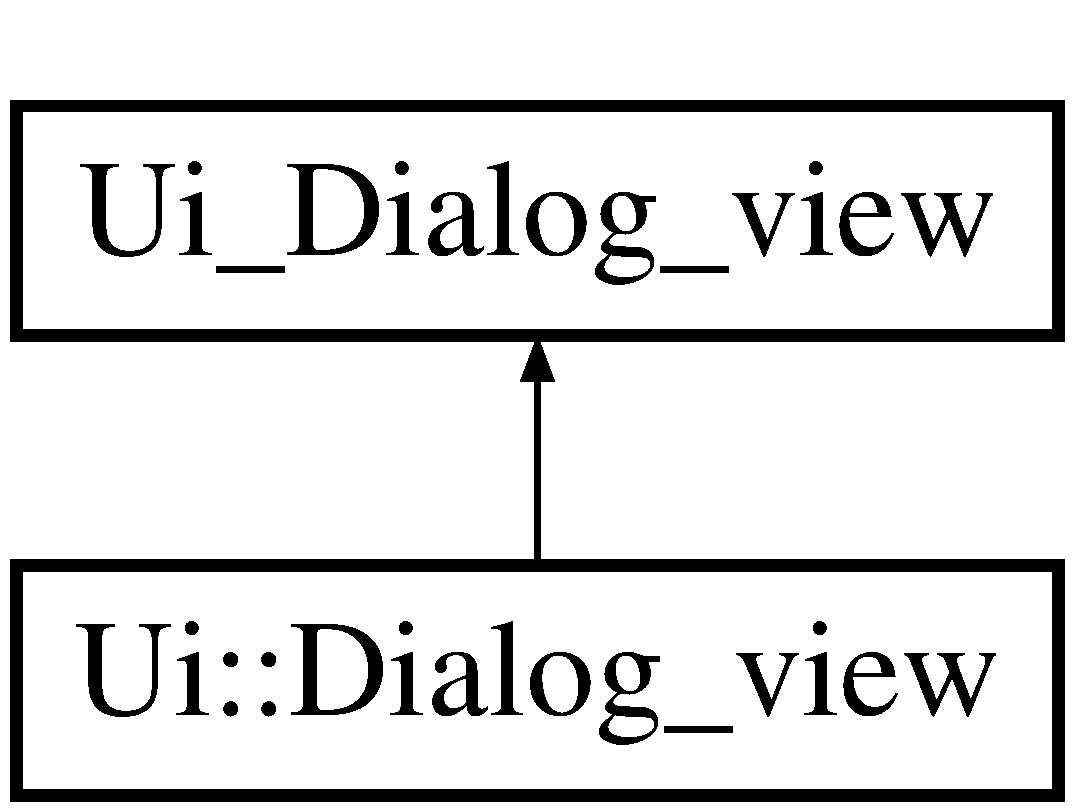
\includegraphics[height=2.000000cm]{class_ui___dialog__view}
\end{center}
\end{figure}
\subsection*{Public Member Functions}
\begin{DoxyCompactItemize}
\item 
void \hyperlink{class_ui___dialog__view_afb94a51d635b2bf69733fd2a4ea41952}{setup\+Ui} (Q\+Dialog $\ast$Dialog\+\_\+view)
\item 
void \hyperlink{class_ui___dialog__view_ae834a6e58c7545bcef4d5f0270b331a8}{retranslate\+Ui} (Q\+Dialog $\ast$Dialog\+\_\+view)
\end{DoxyCompactItemize}
\subsection*{Public Attributes}
\begin{DoxyCompactItemize}
\item 
Q\+Dialog\+Button\+Box $\ast$ \hyperlink{class_ui___dialog__view_a21a8c87fb64b14eee9315ef19a3a3bb3}{button\+Box}
\item 
Q\+Widget $\ast$ \hyperlink{class_ui___dialog__view_a0e98ef3e72073f15b6280ca2537d81ab}{grid\+Layout\+Widget}
\item 
Q\+Grid\+Layout $\ast$ \hyperlink{class_ui___dialog__view_a77d16d3ffbeacd2ea7f8ffef5bd4efc3}{grid\+Layout}
\item 
Q\+Label $\ast$ \hyperlink{class_ui___dialog__view_a504f628127fabf2128d41b30b41fb6b8}{label\+\_\+2}
\item 
Q\+Label $\ast$ \hyperlink{class_ui___dialog__view_a7707206ee512ad1f786ed09affc4eb4d}{label}
\item 
Q\+Double\+Spin\+Box $\ast$ \hyperlink{class_ui___dialog__view_ae5840f6fd0b53493f85a37dcef58c403}{Eyes\+X\+Spin\+Box}
\item 
Q\+Label $\ast$ \hyperlink{class_ui___dialog__view_af3b0c37547a69ec18c44042dd3375891}{label\+\_\+3}
\item 
Q\+Double\+Spin\+Box $\ast$ \hyperlink{class_ui___dialog__view_ab168044e11d249b7a1691544cb0a9a78}{Eyes\+Y\+Spin\+Box}
\item 
Q\+Double\+Spin\+Box $\ast$ \hyperlink{class_ui___dialog__view_ab57dcc3630e280bf882e0d2112536570}{Eyes\+Z\+Spin\+Box}
\item 
Q\+Widget $\ast$ \hyperlink{class_ui___dialog__view_aa6d06ff1a4eae6c50829603637aa6ca8}{grid\+Layout\+Widget\+\_\+2}
\item 
Q\+Grid\+Layout $\ast$ \hyperlink{class_ui___dialog__view_afca9ea5a2e97534872dbe646959e84fd}{grid\+Layout\+\_\+2}
\item 
Q\+Label $\ast$ \hyperlink{class_ui___dialog__view_adaacfa86807c44a8d109094dc59cf9ee}{label\+\_\+4}
\item 
Q\+Label $\ast$ \hyperlink{class_ui___dialog__view_abf2ec29f6da83bbac98d9fca33ab3826}{label\+\_\+5}
\item 
Q\+Double\+Spin\+Box $\ast$ \hyperlink{class_ui___dialog__view_a24813e55f1437289dd4cdd90780dded6}{direct\+X\+Spin\+Box}
\item 
Q\+Label $\ast$ \hyperlink{class_ui___dialog__view_ae3bba8bcf5013ea73da92adc6cd9384f}{label\+\_\+6}
\item 
Q\+Double\+Spin\+Box $\ast$ \hyperlink{class_ui___dialog__view_a96ef0cc5874bf7279969cc8a42ab4638}{direct\+Y\+Spin\+Box}
\item 
Q\+Double\+Spin\+Box $\ast$ \hyperlink{class_ui___dialog__view_aec4dbf7f3b1f9d0491fcd20d31767881}{direct\+Z\+Spin\+Box}
\end{DoxyCompactItemize}


\subsection{Member Function Documentation}
\hypertarget{class_ui___dialog__view_ae834a6e58c7545bcef4d5f0270b331a8}{}\label{class_ui___dialog__view_ae834a6e58c7545bcef4d5f0270b331a8} 
\index{Ui\+\_\+\+Dialog\+\_\+view@{Ui\+\_\+\+Dialog\+\_\+view}!retranslate\+Ui@{retranslate\+Ui}}
\index{retranslate\+Ui@{retranslate\+Ui}!Ui\+\_\+\+Dialog\+\_\+view@{Ui\+\_\+\+Dialog\+\_\+view}}
\subsubsection{\texorpdfstring{retranslate\+Ui()}{retranslateUi()}}
{\footnotesize\ttfamily void Ui\+\_\+\+Dialog\+\_\+view\+::retranslate\+Ui (\begin{DoxyParamCaption}\item[{Q\+Dialog $\ast$}]{Dialog\+\_\+view }\end{DoxyParamCaption})\hspace{0.3cm}{\ttfamily [inline]}}

\hypertarget{class_ui___dialog__view_afb94a51d635b2bf69733fd2a4ea41952}{}\label{class_ui___dialog__view_afb94a51d635b2bf69733fd2a4ea41952} 
\index{Ui\+\_\+\+Dialog\+\_\+view@{Ui\+\_\+\+Dialog\+\_\+view}!setup\+Ui@{setup\+Ui}}
\index{setup\+Ui@{setup\+Ui}!Ui\+\_\+\+Dialog\+\_\+view@{Ui\+\_\+\+Dialog\+\_\+view}}
\subsubsection{\texorpdfstring{setup\+Ui()}{setupUi()}}
{\footnotesize\ttfamily void Ui\+\_\+\+Dialog\+\_\+view\+::setup\+Ui (\begin{DoxyParamCaption}\item[{Q\+Dialog $\ast$}]{Dialog\+\_\+view }\end{DoxyParamCaption})\hspace{0.3cm}{\ttfamily [inline]}}



\subsection{Member Data Documentation}
\hypertarget{class_ui___dialog__view_a21a8c87fb64b14eee9315ef19a3a3bb3}{}\label{class_ui___dialog__view_a21a8c87fb64b14eee9315ef19a3a3bb3} 
\index{Ui\+\_\+\+Dialog\+\_\+view@{Ui\+\_\+\+Dialog\+\_\+view}!button\+Box@{button\+Box}}
\index{button\+Box@{button\+Box}!Ui\+\_\+\+Dialog\+\_\+view@{Ui\+\_\+\+Dialog\+\_\+view}}
\subsubsection{\texorpdfstring{button\+Box}{buttonBox}}
{\footnotesize\ttfamily Q\+Dialog\+Button\+Box$\ast$ Ui\+\_\+\+Dialog\+\_\+view\+::button\+Box}

\hypertarget{class_ui___dialog__view_a24813e55f1437289dd4cdd90780dded6}{}\label{class_ui___dialog__view_a24813e55f1437289dd4cdd90780dded6} 
\index{Ui\+\_\+\+Dialog\+\_\+view@{Ui\+\_\+\+Dialog\+\_\+view}!direct\+X\+Spin\+Box@{direct\+X\+Spin\+Box}}
\index{direct\+X\+Spin\+Box@{direct\+X\+Spin\+Box}!Ui\+\_\+\+Dialog\+\_\+view@{Ui\+\_\+\+Dialog\+\_\+view}}
\subsubsection{\texorpdfstring{direct\+X\+Spin\+Box}{directXSpinBox}}
{\footnotesize\ttfamily Q\+Double\+Spin\+Box$\ast$ Ui\+\_\+\+Dialog\+\_\+view\+::direct\+X\+Spin\+Box}

\hypertarget{class_ui___dialog__view_a96ef0cc5874bf7279969cc8a42ab4638}{}\label{class_ui___dialog__view_a96ef0cc5874bf7279969cc8a42ab4638} 
\index{Ui\+\_\+\+Dialog\+\_\+view@{Ui\+\_\+\+Dialog\+\_\+view}!direct\+Y\+Spin\+Box@{direct\+Y\+Spin\+Box}}
\index{direct\+Y\+Spin\+Box@{direct\+Y\+Spin\+Box}!Ui\+\_\+\+Dialog\+\_\+view@{Ui\+\_\+\+Dialog\+\_\+view}}
\subsubsection{\texorpdfstring{direct\+Y\+Spin\+Box}{directYSpinBox}}
{\footnotesize\ttfamily Q\+Double\+Spin\+Box$\ast$ Ui\+\_\+\+Dialog\+\_\+view\+::direct\+Y\+Spin\+Box}

\hypertarget{class_ui___dialog__view_aec4dbf7f3b1f9d0491fcd20d31767881}{}\label{class_ui___dialog__view_aec4dbf7f3b1f9d0491fcd20d31767881} 
\index{Ui\+\_\+\+Dialog\+\_\+view@{Ui\+\_\+\+Dialog\+\_\+view}!direct\+Z\+Spin\+Box@{direct\+Z\+Spin\+Box}}
\index{direct\+Z\+Spin\+Box@{direct\+Z\+Spin\+Box}!Ui\+\_\+\+Dialog\+\_\+view@{Ui\+\_\+\+Dialog\+\_\+view}}
\subsubsection{\texorpdfstring{direct\+Z\+Spin\+Box}{directZSpinBox}}
{\footnotesize\ttfamily Q\+Double\+Spin\+Box$\ast$ Ui\+\_\+\+Dialog\+\_\+view\+::direct\+Z\+Spin\+Box}

\hypertarget{class_ui___dialog__view_ae5840f6fd0b53493f85a37dcef58c403}{}\label{class_ui___dialog__view_ae5840f6fd0b53493f85a37dcef58c403} 
\index{Ui\+\_\+\+Dialog\+\_\+view@{Ui\+\_\+\+Dialog\+\_\+view}!Eyes\+X\+Spin\+Box@{Eyes\+X\+Spin\+Box}}
\index{Eyes\+X\+Spin\+Box@{Eyes\+X\+Spin\+Box}!Ui\+\_\+\+Dialog\+\_\+view@{Ui\+\_\+\+Dialog\+\_\+view}}
\subsubsection{\texorpdfstring{Eyes\+X\+Spin\+Box}{EyesXSpinBox}}
{\footnotesize\ttfamily Q\+Double\+Spin\+Box$\ast$ Ui\+\_\+\+Dialog\+\_\+view\+::\+Eyes\+X\+Spin\+Box}

\hypertarget{class_ui___dialog__view_ab168044e11d249b7a1691544cb0a9a78}{}\label{class_ui___dialog__view_ab168044e11d249b7a1691544cb0a9a78} 
\index{Ui\+\_\+\+Dialog\+\_\+view@{Ui\+\_\+\+Dialog\+\_\+view}!Eyes\+Y\+Spin\+Box@{Eyes\+Y\+Spin\+Box}}
\index{Eyes\+Y\+Spin\+Box@{Eyes\+Y\+Spin\+Box}!Ui\+\_\+\+Dialog\+\_\+view@{Ui\+\_\+\+Dialog\+\_\+view}}
\subsubsection{\texorpdfstring{Eyes\+Y\+Spin\+Box}{EyesYSpinBox}}
{\footnotesize\ttfamily Q\+Double\+Spin\+Box$\ast$ Ui\+\_\+\+Dialog\+\_\+view\+::\+Eyes\+Y\+Spin\+Box}

\hypertarget{class_ui___dialog__view_ab57dcc3630e280bf882e0d2112536570}{}\label{class_ui___dialog__view_ab57dcc3630e280bf882e0d2112536570} 
\index{Ui\+\_\+\+Dialog\+\_\+view@{Ui\+\_\+\+Dialog\+\_\+view}!Eyes\+Z\+Spin\+Box@{Eyes\+Z\+Spin\+Box}}
\index{Eyes\+Z\+Spin\+Box@{Eyes\+Z\+Spin\+Box}!Ui\+\_\+\+Dialog\+\_\+view@{Ui\+\_\+\+Dialog\+\_\+view}}
\subsubsection{\texorpdfstring{Eyes\+Z\+Spin\+Box}{EyesZSpinBox}}
{\footnotesize\ttfamily Q\+Double\+Spin\+Box$\ast$ Ui\+\_\+\+Dialog\+\_\+view\+::\+Eyes\+Z\+Spin\+Box}

\hypertarget{class_ui___dialog__view_a77d16d3ffbeacd2ea7f8ffef5bd4efc3}{}\label{class_ui___dialog__view_a77d16d3ffbeacd2ea7f8ffef5bd4efc3} 
\index{Ui\+\_\+\+Dialog\+\_\+view@{Ui\+\_\+\+Dialog\+\_\+view}!grid\+Layout@{grid\+Layout}}
\index{grid\+Layout@{grid\+Layout}!Ui\+\_\+\+Dialog\+\_\+view@{Ui\+\_\+\+Dialog\+\_\+view}}
\subsubsection{\texorpdfstring{grid\+Layout}{gridLayout}}
{\footnotesize\ttfamily Q\+Grid\+Layout$\ast$ Ui\+\_\+\+Dialog\+\_\+view\+::grid\+Layout}

\hypertarget{class_ui___dialog__view_afca9ea5a2e97534872dbe646959e84fd}{}\label{class_ui___dialog__view_afca9ea5a2e97534872dbe646959e84fd} 
\index{Ui\+\_\+\+Dialog\+\_\+view@{Ui\+\_\+\+Dialog\+\_\+view}!grid\+Layout\+\_\+2@{grid\+Layout\+\_\+2}}
\index{grid\+Layout\+\_\+2@{grid\+Layout\+\_\+2}!Ui\+\_\+\+Dialog\+\_\+view@{Ui\+\_\+\+Dialog\+\_\+view}}
\subsubsection{\texorpdfstring{grid\+Layout\+\_\+2}{gridLayout\_2}}
{\footnotesize\ttfamily Q\+Grid\+Layout$\ast$ Ui\+\_\+\+Dialog\+\_\+view\+::grid\+Layout\+\_\+2}

\hypertarget{class_ui___dialog__view_a0e98ef3e72073f15b6280ca2537d81ab}{}\label{class_ui___dialog__view_a0e98ef3e72073f15b6280ca2537d81ab} 
\index{Ui\+\_\+\+Dialog\+\_\+view@{Ui\+\_\+\+Dialog\+\_\+view}!grid\+Layout\+Widget@{grid\+Layout\+Widget}}
\index{grid\+Layout\+Widget@{grid\+Layout\+Widget}!Ui\+\_\+\+Dialog\+\_\+view@{Ui\+\_\+\+Dialog\+\_\+view}}
\subsubsection{\texorpdfstring{grid\+Layout\+Widget}{gridLayoutWidget}}
{\footnotesize\ttfamily Q\+Widget$\ast$ Ui\+\_\+\+Dialog\+\_\+view\+::grid\+Layout\+Widget}

\hypertarget{class_ui___dialog__view_aa6d06ff1a4eae6c50829603637aa6ca8}{}\label{class_ui___dialog__view_aa6d06ff1a4eae6c50829603637aa6ca8} 
\index{Ui\+\_\+\+Dialog\+\_\+view@{Ui\+\_\+\+Dialog\+\_\+view}!grid\+Layout\+Widget\+\_\+2@{grid\+Layout\+Widget\+\_\+2}}
\index{grid\+Layout\+Widget\+\_\+2@{grid\+Layout\+Widget\+\_\+2}!Ui\+\_\+\+Dialog\+\_\+view@{Ui\+\_\+\+Dialog\+\_\+view}}
\subsubsection{\texorpdfstring{grid\+Layout\+Widget\+\_\+2}{gridLayoutWidget\_2}}
{\footnotesize\ttfamily Q\+Widget$\ast$ Ui\+\_\+\+Dialog\+\_\+view\+::grid\+Layout\+Widget\+\_\+2}

\hypertarget{class_ui___dialog__view_a7707206ee512ad1f786ed09affc4eb4d}{}\label{class_ui___dialog__view_a7707206ee512ad1f786ed09affc4eb4d} 
\index{Ui\+\_\+\+Dialog\+\_\+view@{Ui\+\_\+\+Dialog\+\_\+view}!label@{label}}
\index{label@{label}!Ui\+\_\+\+Dialog\+\_\+view@{Ui\+\_\+\+Dialog\+\_\+view}}
\subsubsection{\texorpdfstring{label}{label}}
{\footnotesize\ttfamily Q\+Label$\ast$ Ui\+\_\+\+Dialog\+\_\+view\+::label}

\hypertarget{class_ui___dialog__view_a504f628127fabf2128d41b30b41fb6b8}{}\label{class_ui___dialog__view_a504f628127fabf2128d41b30b41fb6b8} 
\index{Ui\+\_\+\+Dialog\+\_\+view@{Ui\+\_\+\+Dialog\+\_\+view}!label\+\_\+2@{label\+\_\+2}}
\index{label\+\_\+2@{label\+\_\+2}!Ui\+\_\+\+Dialog\+\_\+view@{Ui\+\_\+\+Dialog\+\_\+view}}
\subsubsection{\texorpdfstring{label\+\_\+2}{label\_2}}
{\footnotesize\ttfamily Q\+Label$\ast$ Ui\+\_\+\+Dialog\+\_\+view\+::label\+\_\+2}

\hypertarget{class_ui___dialog__view_af3b0c37547a69ec18c44042dd3375891}{}\label{class_ui___dialog__view_af3b0c37547a69ec18c44042dd3375891} 
\index{Ui\+\_\+\+Dialog\+\_\+view@{Ui\+\_\+\+Dialog\+\_\+view}!label\+\_\+3@{label\+\_\+3}}
\index{label\+\_\+3@{label\+\_\+3}!Ui\+\_\+\+Dialog\+\_\+view@{Ui\+\_\+\+Dialog\+\_\+view}}
\subsubsection{\texorpdfstring{label\+\_\+3}{label\_3}}
{\footnotesize\ttfamily Q\+Label$\ast$ Ui\+\_\+\+Dialog\+\_\+view\+::label\+\_\+3}

\hypertarget{class_ui___dialog__view_adaacfa86807c44a8d109094dc59cf9ee}{}\label{class_ui___dialog__view_adaacfa86807c44a8d109094dc59cf9ee} 
\index{Ui\+\_\+\+Dialog\+\_\+view@{Ui\+\_\+\+Dialog\+\_\+view}!label\+\_\+4@{label\+\_\+4}}
\index{label\+\_\+4@{label\+\_\+4}!Ui\+\_\+\+Dialog\+\_\+view@{Ui\+\_\+\+Dialog\+\_\+view}}
\subsubsection{\texorpdfstring{label\+\_\+4}{label\_4}}
{\footnotesize\ttfamily Q\+Label$\ast$ Ui\+\_\+\+Dialog\+\_\+view\+::label\+\_\+4}

\hypertarget{class_ui___dialog__view_abf2ec29f6da83bbac98d9fca33ab3826}{}\label{class_ui___dialog__view_abf2ec29f6da83bbac98d9fca33ab3826} 
\index{Ui\+\_\+\+Dialog\+\_\+view@{Ui\+\_\+\+Dialog\+\_\+view}!label\+\_\+5@{label\+\_\+5}}
\index{label\+\_\+5@{label\+\_\+5}!Ui\+\_\+\+Dialog\+\_\+view@{Ui\+\_\+\+Dialog\+\_\+view}}
\subsubsection{\texorpdfstring{label\+\_\+5}{label\_5}}
{\footnotesize\ttfamily Q\+Label$\ast$ Ui\+\_\+\+Dialog\+\_\+view\+::label\+\_\+5}

\hypertarget{class_ui___dialog__view_ae3bba8bcf5013ea73da92adc6cd9384f}{}\label{class_ui___dialog__view_ae3bba8bcf5013ea73da92adc6cd9384f} 
\index{Ui\+\_\+\+Dialog\+\_\+view@{Ui\+\_\+\+Dialog\+\_\+view}!label\+\_\+6@{label\+\_\+6}}
\index{label\+\_\+6@{label\+\_\+6}!Ui\+\_\+\+Dialog\+\_\+view@{Ui\+\_\+\+Dialog\+\_\+view}}
\subsubsection{\texorpdfstring{label\+\_\+6}{label\_6}}
{\footnotesize\ttfamily Q\+Label$\ast$ Ui\+\_\+\+Dialog\+\_\+view\+::label\+\_\+6}



The documentation for this class was generated from the following file\+:\begin{DoxyCompactItemize}
\item 
D\+:/\+Q\+T\+\_\+projets/\+Cube\+Menu/\hyperlink{ui__dialog__view_8h}{ui\+\_\+dialog\+\_\+view.\+h}\end{DoxyCompactItemize}

\hypertarget{class_ui___dialog_eyes}{}\section{Ui\+\_\+\+Dialog\+Eyes Class Reference}
\label{class_ui___dialog_eyes}\index{Ui\+\_\+\+Dialog\+Eyes@{Ui\+\_\+\+Dialog\+Eyes}}


{\ttfamily \#include $<$ui\+\_\+dialogeyes.\+h$>$}

Inheritance diagram for Ui\+\_\+\+Dialog\+Eyes\+:\begin{figure}[H]
\begin{center}
\leavevmode
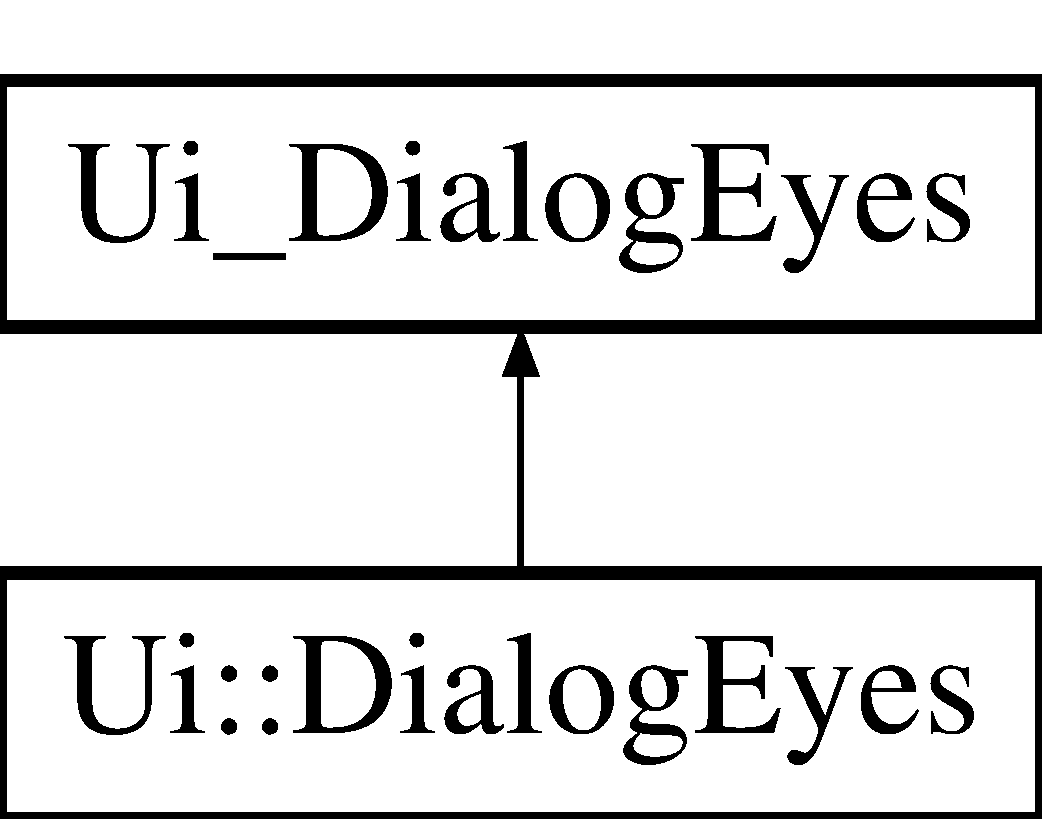
\includegraphics[height=2.000000cm]{class_ui___dialog_eyes}
\end{center}
\end{figure}
\subsection*{Public Member Functions}
\begin{DoxyCompactItemize}
\item 
void \hyperlink{class_ui___dialog_eyes_a51ce884bcab7ca170ca7b45f25dd93be}{setup\+Ui} (Q\+Dialog $\ast$\hyperlink{class_dialog_eyes}{Dialog\+Eyes})
\item 
void \hyperlink{class_ui___dialog_eyes_ac241c0d82e58ce5044e0a76debc206b3}{retranslate\+Ui} (Q\+Dialog $\ast$\hyperlink{class_dialog_eyes}{Dialog\+Eyes})
\end{DoxyCompactItemize}
\subsection*{Public Attributes}
\begin{DoxyCompactItemize}
\item 
Q\+Widget $\ast$ \hyperlink{class_ui___dialog_eyes_a27186a39ae6dc855ac34f50e68590e54}{vertical\+Layout\+Widget\+\_\+3}
\item 
Q\+V\+Box\+Layout $\ast$ \hyperlink{class_ui___dialog_eyes_a894170ae9e75a9d3800072b4ebfa2639}{vertical\+Layout\+\_\+7}
\item 
Q\+Label $\ast$ \hyperlink{class_ui___dialog_eyes_af980b1895bf87b705bf10f401cd75d3f}{label\+\_\+10}
\item 
Q\+Form\+Layout $\ast$ \hyperlink{class_ui___dialog_eyes_a83076edd627b19377863a28f11ff74b2}{form\+Layout}
\item 
Q\+V\+Box\+Layout $\ast$ \hyperlink{class_ui___dialog_eyes_a7268513884026bc8a04b16b04fc41cde}{vertical\+Layout}
\item 
Q\+Label $\ast$ \hyperlink{class_ui___dialog_eyes_a448b37d2a7906fae559cdd59f913c5cb}{label}
\item 
Q\+Grid\+Layout $\ast$ \hyperlink{class_ui___dialog_eyes_a5957bc0bb2476de51bdc5d3670d147f4}{grid\+Layout\+\_\+2}
\item 
Q\+Double\+Spin\+Box $\ast$ \hyperlink{class_ui___dialog_eyes_a0f2e95f66886cb79ba533a3d50501157}{double\+Spin\+Box\+\_\+eyey}
\item 
Q\+Label $\ast$ \hyperlink{class_ui___dialog_eyes_a085f807dc2b0830a9ed847d460887eb5}{label\+\_\+4}
\item 
Q\+Label $\ast$ \hyperlink{class_ui___dialog_eyes_a12773bd4af3d824420d1d6f2a6a1ff8c}{label\+\_\+2}
\item 
Q\+Double\+Spin\+Box $\ast$ \hyperlink{class_ui___dialog_eyes_adc1990f769605d17d2d0dce6b2540130}{double\+Spin\+Box\+\_\+eyez}
\item 
Q\+Double\+Spin\+Box $\ast$ \hyperlink{class_ui___dialog_eyes_aef63991da52508c1b8c4c187cc426626}{double\+Spin\+Box\+\_\+eyex}
\item 
Q\+Label $\ast$ \hyperlink{class_ui___dialog_eyes_a9d88de1f1a79acc44a2e89fafa28e72c}{label\+\_\+3}
\item 
Q\+V\+Box\+Layout $\ast$ \hyperlink{class_ui___dialog_eyes_a72332239b48624787211c642925f9c57}{vertical\+Layout\+\_\+2}
\item 
Q\+Label $\ast$ \hyperlink{class_ui___dialog_eyes_a2baff1eaac5a1f56aa1069ea7338da04}{label\+\_\+5}
\item 
Q\+Grid\+Layout $\ast$ \hyperlink{class_ui___dialog_eyes_aca6d083b4e7f08dde22c47e777a07779}{grid\+Layout\+\_\+3}
\item 
Q\+Label $\ast$ \hyperlink{class_ui___dialog_eyes_ae8541d3c768ed2c09a8bbf8154c1d2f8}{label\+\_\+7}
\item 
Q\+Label $\ast$ \hyperlink{class_ui___dialog_eyes_a70abfa97c9448788a4895316f88c0603}{label\+\_\+8}
\item 
Q\+Label $\ast$ \hyperlink{class_ui___dialog_eyes_ac0330213bbebb84107c2970edb1f8eeb}{label\+\_\+6}
\item 
Q\+Double\+Spin\+Box $\ast$ \hyperlink{class_ui___dialog_eyes_aababf5f01ccf0009e1131403900b1cae}{double\+Spin\+Box\+\_\+dx}
\item 
Q\+Double\+Spin\+Box $\ast$ \hyperlink{class_ui___dialog_eyes_a118542559787e7f13ed3e02ff70adb84}{double\+Spin\+Box\+\_\+dy}
\item 
Q\+Double\+Spin\+Box $\ast$ \hyperlink{class_ui___dialog_eyes_a82dfb342b687d0b2a377eb1f77c9682a}{double\+Spin\+Box\+\_\+dz}
\item 
Q\+Dialog\+Button\+Box $\ast$ \hyperlink{class_ui___dialog_eyes_ae39373bb3f9ab9b0ccc6dd2d999667c6}{button\+Box}
\item 
Q\+Push\+Button $\ast$ \hyperlink{class_ui___dialog_eyes_abf6a5d6aa5f67da211f2ff9a573ad4ac}{push\+Button\+\_\+reset}
\end{DoxyCompactItemize}


\subsection{Member Function Documentation}
\hypertarget{class_ui___dialog_eyes_ac241c0d82e58ce5044e0a76debc206b3}{}\label{class_ui___dialog_eyes_ac241c0d82e58ce5044e0a76debc206b3} 
\index{Ui\+\_\+\+Dialog\+Eyes@{Ui\+\_\+\+Dialog\+Eyes}!retranslate\+Ui@{retranslate\+Ui}}
\index{retranslate\+Ui@{retranslate\+Ui}!Ui\+\_\+\+Dialog\+Eyes@{Ui\+\_\+\+Dialog\+Eyes}}
\subsubsection{\texorpdfstring{retranslate\+Ui()}{retranslateUi()}}
{\footnotesize\ttfamily void Ui\+\_\+\+Dialog\+Eyes\+::retranslate\+Ui (\begin{DoxyParamCaption}\item[{Q\+Dialog $\ast$}]{Dialog\+Eyes }\end{DoxyParamCaption})\hspace{0.3cm}{\ttfamily [inline]}}

\hypertarget{class_ui___dialog_eyes_a51ce884bcab7ca170ca7b45f25dd93be}{}\label{class_ui___dialog_eyes_a51ce884bcab7ca170ca7b45f25dd93be} 
\index{Ui\+\_\+\+Dialog\+Eyes@{Ui\+\_\+\+Dialog\+Eyes}!setup\+Ui@{setup\+Ui}}
\index{setup\+Ui@{setup\+Ui}!Ui\+\_\+\+Dialog\+Eyes@{Ui\+\_\+\+Dialog\+Eyes}}
\subsubsection{\texorpdfstring{setup\+Ui()}{setupUi()}}
{\footnotesize\ttfamily void Ui\+\_\+\+Dialog\+Eyes\+::setup\+Ui (\begin{DoxyParamCaption}\item[{Q\+Dialog $\ast$}]{Dialog\+Eyes }\end{DoxyParamCaption})\hspace{0.3cm}{\ttfamily [inline]}}



\subsection{Member Data Documentation}
\hypertarget{class_ui___dialog_eyes_ae39373bb3f9ab9b0ccc6dd2d999667c6}{}\label{class_ui___dialog_eyes_ae39373bb3f9ab9b0ccc6dd2d999667c6} 
\index{Ui\+\_\+\+Dialog\+Eyes@{Ui\+\_\+\+Dialog\+Eyes}!button\+Box@{button\+Box}}
\index{button\+Box@{button\+Box}!Ui\+\_\+\+Dialog\+Eyes@{Ui\+\_\+\+Dialog\+Eyes}}
\subsubsection{\texorpdfstring{button\+Box}{buttonBox}}
{\footnotesize\ttfamily Q\+Dialog\+Button\+Box$\ast$ Ui\+\_\+\+Dialog\+Eyes\+::button\+Box}

\hypertarget{class_ui___dialog_eyes_aababf5f01ccf0009e1131403900b1cae}{}\label{class_ui___dialog_eyes_aababf5f01ccf0009e1131403900b1cae} 
\index{Ui\+\_\+\+Dialog\+Eyes@{Ui\+\_\+\+Dialog\+Eyes}!double\+Spin\+Box\+\_\+dx@{double\+Spin\+Box\+\_\+dx}}
\index{double\+Spin\+Box\+\_\+dx@{double\+Spin\+Box\+\_\+dx}!Ui\+\_\+\+Dialog\+Eyes@{Ui\+\_\+\+Dialog\+Eyes}}
\subsubsection{\texorpdfstring{double\+Spin\+Box\+\_\+dx}{doubleSpinBox\_dx}}
{\footnotesize\ttfamily Q\+Double\+Spin\+Box$\ast$ Ui\+\_\+\+Dialog\+Eyes\+::double\+Spin\+Box\+\_\+dx}

\hypertarget{class_ui___dialog_eyes_a118542559787e7f13ed3e02ff70adb84}{}\label{class_ui___dialog_eyes_a118542559787e7f13ed3e02ff70adb84} 
\index{Ui\+\_\+\+Dialog\+Eyes@{Ui\+\_\+\+Dialog\+Eyes}!double\+Spin\+Box\+\_\+dy@{double\+Spin\+Box\+\_\+dy}}
\index{double\+Spin\+Box\+\_\+dy@{double\+Spin\+Box\+\_\+dy}!Ui\+\_\+\+Dialog\+Eyes@{Ui\+\_\+\+Dialog\+Eyes}}
\subsubsection{\texorpdfstring{double\+Spin\+Box\+\_\+dy}{doubleSpinBox\_dy}}
{\footnotesize\ttfamily Q\+Double\+Spin\+Box$\ast$ Ui\+\_\+\+Dialog\+Eyes\+::double\+Spin\+Box\+\_\+dy}

\hypertarget{class_ui___dialog_eyes_a82dfb342b687d0b2a377eb1f77c9682a}{}\label{class_ui___dialog_eyes_a82dfb342b687d0b2a377eb1f77c9682a} 
\index{Ui\+\_\+\+Dialog\+Eyes@{Ui\+\_\+\+Dialog\+Eyes}!double\+Spin\+Box\+\_\+dz@{double\+Spin\+Box\+\_\+dz}}
\index{double\+Spin\+Box\+\_\+dz@{double\+Spin\+Box\+\_\+dz}!Ui\+\_\+\+Dialog\+Eyes@{Ui\+\_\+\+Dialog\+Eyes}}
\subsubsection{\texorpdfstring{double\+Spin\+Box\+\_\+dz}{doubleSpinBox\_dz}}
{\footnotesize\ttfamily Q\+Double\+Spin\+Box$\ast$ Ui\+\_\+\+Dialog\+Eyes\+::double\+Spin\+Box\+\_\+dz}

\hypertarget{class_ui___dialog_eyes_aef63991da52508c1b8c4c187cc426626}{}\label{class_ui___dialog_eyes_aef63991da52508c1b8c4c187cc426626} 
\index{Ui\+\_\+\+Dialog\+Eyes@{Ui\+\_\+\+Dialog\+Eyes}!double\+Spin\+Box\+\_\+eyex@{double\+Spin\+Box\+\_\+eyex}}
\index{double\+Spin\+Box\+\_\+eyex@{double\+Spin\+Box\+\_\+eyex}!Ui\+\_\+\+Dialog\+Eyes@{Ui\+\_\+\+Dialog\+Eyes}}
\subsubsection{\texorpdfstring{double\+Spin\+Box\+\_\+eyex}{doubleSpinBox\_eyex}}
{\footnotesize\ttfamily Q\+Double\+Spin\+Box$\ast$ Ui\+\_\+\+Dialog\+Eyes\+::double\+Spin\+Box\+\_\+eyex}

\hypertarget{class_ui___dialog_eyes_a0f2e95f66886cb79ba533a3d50501157}{}\label{class_ui___dialog_eyes_a0f2e95f66886cb79ba533a3d50501157} 
\index{Ui\+\_\+\+Dialog\+Eyes@{Ui\+\_\+\+Dialog\+Eyes}!double\+Spin\+Box\+\_\+eyey@{double\+Spin\+Box\+\_\+eyey}}
\index{double\+Spin\+Box\+\_\+eyey@{double\+Spin\+Box\+\_\+eyey}!Ui\+\_\+\+Dialog\+Eyes@{Ui\+\_\+\+Dialog\+Eyes}}
\subsubsection{\texorpdfstring{double\+Spin\+Box\+\_\+eyey}{doubleSpinBox\_eyey}}
{\footnotesize\ttfamily Q\+Double\+Spin\+Box$\ast$ Ui\+\_\+\+Dialog\+Eyes\+::double\+Spin\+Box\+\_\+eyey}

\hypertarget{class_ui___dialog_eyes_adc1990f769605d17d2d0dce6b2540130}{}\label{class_ui___dialog_eyes_adc1990f769605d17d2d0dce6b2540130} 
\index{Ui\+\_\+\+Dialog\+Eyes@{Ui\+\_\+\+Dialog\+Eyes}!double\+Spin\+Box\+\_\+eyez@{double\+Spin\+Box\+\_\+eyez}}
\index{double\+Spin\+Box\+\_\+eyez@{double\+Spin\+Box\+\_\+eyez}!Ui\+\_\+\+Dialog\+Eyes@{Ui\+\_\+\+Dialog\+Eyes}}
\subsubsection{\texorpdfstring{double\+Spin\+Box\+\_\+eyez}{doubleSpinBox\_eyez}}
{\footnotesize\ttfamily Q\+Double\+Spin\+Box$\ast$ Ui\+\_\+\+Dialog\+Eyes\+::double\+Spin\+Box\+\_\+eyez}

\hypertarget{class_ui___dialog_eyes_a83076edd627b19377863a28f11ff74b2}{}\label{class_ui___dialog_eyes_a83076edd627b19377863a28f11ff74b2} 
\index{Ui\+\_\+\+Dialog\+Eyes@{Ui\+\_\+\+Dialog\+Eyes}!form\+Layout@{form\+Layout}}
\index{form\+Layout@{form\+Layout}!Ui\+\_\+\+Dialog\+Eyes@{Ui\+\_\+\+Dialog\+Eyes}}
\subsubsection{\texorpdfstring{form\+Layout}{formLayout}}
{\footnotesize\ttfamily Q\+Form\+Layout$\ast$ Ui\+\_\+\+Dialog\+Eyes\+::form\+Layout}

\hypertarget{class_ui___dialog_eyes_a5957bc0bb2476de51bdc5d3670d147f4}{}\label{class_ui___dialog_eyes_a5957bc0bb2476de51bdc5d3670d147f4} 
\index{Ui\+\_\+\+Dialog\+Eyes@{Ui\+\_\+\+Dialog\+Eyes}!grid\+Layout\+\_\+2@{grid\+Layout\+\_\+2}}
\index{grid\+Layout\+\_\+2@{grid\+Layout\+\_\+2}!Ui\+\_\+\+Dialog\+Eyes@{Ui\+\_\+\+Dialog\+Eyes}}
\subsubsection{\texorpdfstring{grid\+Layout\+\_\+2}{gridLayout\_2}}
{\footnotesize\ttfamily Q\+Grid\+Layout$\ast$ Ui\+\_\+\+Dialog\+Eyes\+::grid\+Layout\+\_\+2}

\hypertarget{class_ui___dialog_eyes_aca6d083b4e7f08dde22c47e777a07779}{}\label{class_ui___dialog_eyes_aca6d083b4e7f08dde22c47e777a07779} 
\index{Ui\+\_\+\+Dialog\+Eyes@{Ui\+\_\+\+Dialog\+Eyes}!grid\+Layout\+\_\+3@{grid\+Layout\+\_\+3}}
\index{grid\+Layout\+\_\+3@{grid\+Layout\+\_\+3}!Ui\+\_\+\+Dialog\+Eyes@{Ui\+\_\+\+Dialog\+Eyes}}
\subsubsection{\texorpdfstring{grid\+Layout\+\_\+3}{gridLayout\_3}}
{\footnotesize\ttfamily Q\+Grid\+Layout$\ast$ Ui\+\_\+\+Dialog\+Eyes\+::grid\+Layout\+\_\+3}

\hypertarget{class_ui___dialog_eyes_a448b37d2a7906fae559cdd59f913c5cb}{}\label{class_ui___dialog_eyes_a448b37d2a7906fae559cdd59f913c5cb} 
\index{Ui\+\_\+\+Dialog\+Eyes@{Ui\+\_\+\+Dialog\+Eyes}!label@{label}}
\index{label@{label}!Ui\+\_\+\+Dialog\+Eyes@{Ui\+\_\+\+Dialog\+Eyes}}
\subsubsection{\texorpdfstring{label}{label}}
{\footnotesize\ttfamily Q\+Label$\ast$ Ui\+\_\+\+Dialog\+Eyes\+::label}

\hypertarget{class_ui___dialog_eyes_af980b1895bf87b705bf10f401cd75d3f}{}\label{class_ui___dialog_eyes_af980b1895bf87b705bf10f401cd75d3f} 
\index{Ui\+\_\+\+Dialog\+Eyes@{Ui\+\_\+\+Dialog\+Eyes}!label\+\_\+10@{label\+\_\+10}}
\index{label\+\_\+10@{label\+\_\+10}!Ui\+\_\+\+Dialog\+Eyes@{Ui\+\_\+\+Dialog\+Eyes}}
\subsubsection{\texorpdfstring{label\+\_\+10}{label\_10}}
{\footnotesize\ttfamily Q\+Label$\ast$ Ui\+\_\+\+Dialog\+Eyes\+::label\+\_\+10}

\hypertarget{class_ui___dialog_eyes_a12773bd4af3d824420d1d6f2a6a1ff8c}{}\label{class_ui___dialog_eyes_a12773bd4af3d824420d1d6f2a6a1ff8c} 
\index{Ui\+\_\+\+Dialog\+Eyes@{Ui\+\_\+\+Dialog\+Eyes}!label\+\_\+2@{label\+\_\+2}}
\index{label\+\_\+2@{label\+\_\+2}!Ui\+\_\+\+Dialog\+Eyes@{Ui\+\_\+\+Dialog\+Eyes}}
\subsubsection{\texorpdfstring{label\+\_\+2}{label\_2}}
{\footnotesize\ttfamily Q\+Label$\ast$ Ui\+\_\+\+Dialog\+Eyes\+::label\+\_\+2}

\hypertarget{class_ui___dialog_eyes_a9d88de1f1a79acc44a2e89fafa28e72c}{}\label{class_ui___dialog_eyes_a9d88de1f1a79acc44a2e89fafa28e72c} 
\index{Ui\+\_\+\+Dialog\+Eyes@{Ui\+\_\+\+Dialog\+Eyes}!label\+\_\+3@{label\+\_\+3}}
\index{label\+\_\+3@{label\+\_\+3}!Ui\+\_\+\+Dialog\+Eyes@{Ui\+\_\+\+Dialog\+Eyes}}
\subsubsection{\texorpdfstring{label\+\_\+3}{label\_3}}
{\footnotesize\ttfamily Q\+Label$\ast$ Ui\+\_\+\+Dialog\+Eyes\+::label\+\_\+3}

\hypertarget{class_ui___dialog_eyes_a085f807dc2b0830a9ed847d460887eb5}{}\label{class_ui___dialog_eyes_a085f807dc2b0830a9ed847d460887eb5} 
\index{Ui\+\_\+\+Dialog\+Eyes@{Ui\+\_\+\+Dialog\+Eyes}!label\+\_\+4@{label\+\_\+4}}
\index{label\+\_\+4@{label\+\_\+4}!Ui\+\_\+\+Dialog\+Eyes@{Ui\+\_\+\+Dialog\+Eyes}}
\subsubsection{\texorpdfstring{label\+\_\+4}{label\_4}}
{\footnotesize\ttfamily Q\+Label$\ast$ Ui\+\_\+\+Dialog\+Eyes\+::label\+\_\+4}

\hypertarget{class_ui___dialog_eyes_a2baff1eaac5a1f56aa1069ea7338da04}{}\label{class_ui___dialog_eyes_a2baff1eaac5a1f56aa1069ea7338da04} 
\index{Ui\+\_\+\+Dialog\+Eyes@{Ui\+\_\+\+Dialog\+Eyes}!label\+\_\+5@{label\+\_\+5}}
\index{label\+\_\+5@{label\+\_\+5}!Ui\+\_\+\+Dialog\+Eyes@{Ui\+\_\+\+Dialog\+Eyes}}
\subsubsection{\texorpdfstring{label\+\_\+5}{label\_5}}
{\footnotesize\ttfamily Q\+Label$\ast$ Ui\+\_\+\+Dialog\+Eyes\+::label\+\_\+5}

\hypertarget{class_ui___dialog_eyes_ac0330213bbebb84107c2970edb1f8eeb}{}\label{class_ui___dialog_eyes_ac0330213bbebb84107c2970edb1f8eeb} 
\index{Ui\+\_\+\+Dialog\+Eyes@{Ui\+\_\+\+Dialog\+Eyes}!label\+\_\+6@{label\+\_\+6}}
\index{label\+\_\+6@{label\+\_\+6}!Ui\+\_\+\+Dialog\+Eyes@{Ui\+\_\+\+Dialog\+Eyes}}
\subsubsection{\texorpdfstring{label\+\_\+6}{label\_6}}
{\footnotesize\ttfamily Q\+Label$\ast$ Ui\+\_\+\+Dialog\+Eyes\+::label\+\_\+6}

\hypertarget{class_ui___dialog_eyes_ae8541d3c768ed2c09a8bbf8154c1d2f8}{}\label{class_ui___dialog_eyes_ae8541d3c768ed2c09a8bbf8154c1d2f8} 
\index{Ui\+\_\+\+Dialog\+Eyes@{Ui\+\_\+\+Dialog\+Eyes}!label\+\_\+7@{label\+\_\+7}}
\index{label\+\_\+7@{label\+\_\+7}!Ui\+\_\+\+Dialog\+Eyes@{Ui\+\_\+\+Dialog\+Eyes}}
\subsubsection{\texorpdfstring{label\+\_\+7}{label\_7}}
{\footnotesize\ttfamily Q\+Label$\ast$ Ui\+\_\+\+Dialog\+Eyes\+::label\+\_\+7}

\hypertarget{class_ui___dialog_eyes_a70abfa97c9448788a4895316f88c0603}{}\label{class_ui___dialog_eyes_a70abfa97c9448788a4895316f88c0603} 
\index{Ui\+\_\+\+Dialog\+Eyes@{Ui\+\_\+\+Dialog\+Eyes}!label\+\_\+8@{label\+\_\+8}}
\index{label\+\_\+8@{label\+\_\+8}!Ui\+\_\+\+Dialog\+Eyes@{Ui\+\_\+\+Dialog\+Eyes}}
\subsubsection{\texorpdfstring{label\+\_\+8}{label\_8}}
{\footnotesize\ttfamily Q\+Label$\ast$ Ui\+\_\+\+Dialog\+Eyes\+::label\+\_\+8}

\hypertarget{class_ui___dialog_eyes_abf6a5d6aa5f67da211f2ff9a573ad4ac}{}\label{class_ui___dialog_eyes_abf6a5d6aa5f67da211f2ff9a573ad4ac} 
\index{Ui\+\_\+\+Dialog\+Eyes@{Ui\+\_\+\+Dialog\+Eyes}!push\+Button\+\_\+reset@{push\+Button\+\_\+reset}}
\index{push\+Button\+\_\+reset@{push\+Button\+\_\+reset}!Ui\+\_\+\+Dialog\+Eyes@{Ui\+\_\+\+Dialog\+Eyes}}
\subsubsection{\texorpdfstring{push\+Button\+\_\+reset}{pushButton\_reset}}
{\footnotesize\ttfamily Q\+Push\+Button$\ast$ Ui\+\_\+\+Dialog\+Eyes\+::push\+Button\+\_\+reset}

\hypertarget{class_ui___dialog_eyes_a7268513884026bc8a04b16b04fc41cde}{}\label{class_ui___dialog_eyes_a7268513884026bc8a04b16b04fc41cde} 
\index{Ui\+\_\+\+Dialog\+Eyes@{Ui\+\_\+\+Dialog\+Eyes}!vertical\+Layout@{vertical\+Layout}}
\index{vertical\+Layout@{vertical\+Layout}!Ui\+\_\+\+Dialog\+Eyes@{Ui\+\_\+\+Dialog\+Eyes}}
\subsubsection{\texorpdfstring{vertical\+Layout}{verticalLayout}}
{\footnotesize\ttfamily Q\+V\+Box\+Layout$\ast$ Ui\+\_\+\+Dialog\+Eyes\+::vertical\+Layout}

\hypertarget{class_ui___dialog_eyes_a72332239b48624787211c642925f9c57}{}\label{class_ui___dialog_eyes_a72332239b48624787211c642925f9c57} 
\index{Ui\+\_\+\+Dialog\+Eyes@{Ui\+\_\+\+Dialog\+Eyes}!vertical\+Layout\+\_\+2@{vertical\+Layout\+\_\+2}}
\index{vertical\+Layout\+\_\+2@{vertical\+Layout\+\_\+2}!Ui\+\_\+\+Dialog\+Eyes@{Ui\+\_\+\+Dialog\+Eyes}}
\subsubsection{\texorpdfstring{vertical\+Layout\+\_\+2}{verticalLayout\_2}}
{\footnotesize\ttfamily Q\+V\+Box\+Layout$\ast$ Ui\+\_\+\+Dialog\+Eyes\+::vertical\+Layout\+\_\+2}

\hypertarget{class_ui___dialog_eyes_a894170ae9e75a9d3800072b4ebfa2639}{}\label{class_ui___dialog_eyes_a894170ae9e75a9d3800072b4ebfa2639} 
\index{Ui\+\_\+\+Dialog\+Eyes@{Ui\+\_\+\+Dialog\+Eyes}!vertical\+Layout\+\_\+7@{vertical\+Layout\+\_\+7}}
\index{vertical\+Layout\+\_\+7@{vertical\+Layout\+\_\+7}!Ui\+\_\+\+Dialog\+Eyes@{Ui\+\_\+\+Dialog\+Eyes}}
\subsubsection{\texorpdfstring{vertical\+Layout\+\_\+7}{verticalLayout\_7}}
{\footnotesize\ttfamily Q\+V\+Box\+Layout$\ast$ Ui\+\_\+\+Dialog\+Eyes\+::vertical\+Layout\+\_\+7}

\hypertarget{class_ui___dialog_eyes_a27186a39ae6dc855ac34f50e68590e54}{}\label{class_ui___dialog_eyes_a27186a39ae6dc855ac34f50e68590e54} 
\index{Ui\+\_\+\+Dialog\+Eyes@{Ui\+\_\+\+Dialog\+Eyes}!vertical\+Layout\+Widget\+\_\+3@{vertical\+Layout\+Widget\+\_\+3}}
\index{vertical\+Layout\+Widget\+\_\+3@{vertical\+Layout\+Widget\+\_\+3}!Ui\+\_\+\+Dialog\+Eyes@{Ui\+\_\+\+Dialog\+Eyes}}
\subsubsection{\texorpdfstring{vertical\+Layout\+Widget\+\_\+3}{verticalLayoutWidget\_3}}
{\footnotesize\ttfamily Q\+Widget$\ast$ Ui\+\_\+\+Dialog\+Eyes\+::vertical\+Layout\+Widget\+\_\+3}



The documentation for this class was generated from the following file\+:\begin{DoxyCompactItemize}
\item 
D\+:/\+Q\+T\+\_\+projets/\+Cube\+Menu/\hyperlink{ui__dialogeyes_8h}{ui\+\_\+dialogeyes.\+h}\end{DoxyCompactItemize}

\hypertarget{class_ui___main_window}{}\section{Ui\+\_\+\+Main\+Window Class Reference}
\label{class_ui___main_window}\index{Ui\+\_\+\+Main\+Window@{Ui\+\_\+\+Main\+Window}}


{\ttfamily \#include $<$ui\+\_\+mainwindow.\+h$>$}

Inheritance diagram for Ui\+\_\+\+Main\+Window\+:\begin{figure}[H]
\begin{center}
\leavevmode
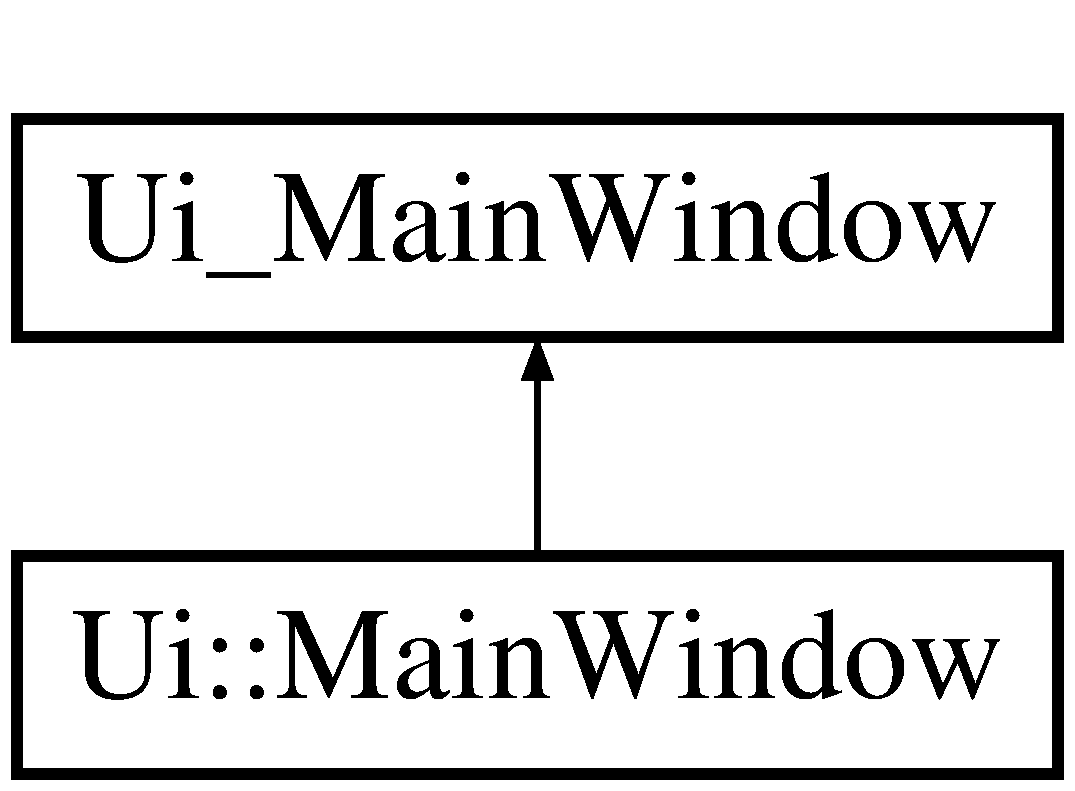
\includegraphics[height=2.000000cm]{class_ui___main_window}
\end{center}
\end{figure}
\subsection*{Public Member Functions}
\begin{DoxyCompactItemize}
\item 
void \hyperlink{class_ui___main_window_acf4a0872c4c77d8f43a2ec66ed849b58}{setup\+Ui} (Q\+Main\+Window $\ast$\hyperlink{class_main_window}{Main\+Window})
\item 
void \hyperlink{class_ui___main_window_a097dd160c3534a204904cb374412c618}{retranslate\+Ui} (Q\+Main\+Window $\ast$\hyperlink{class_main_window}{Main\+Window})
\end{DoxyCompactItemize}
\subsection*{Public Attributes}
\begin{DoxyCompactItemize}
\item 
Q\+Action $\ast$ \hyperlink{class_ui___main_window_a01dc6ef8ed9c1a2ade1b6cda5f441c0a}{action\+Choose\+\_\+\+Parameters}
\item 
Q\+Action $\ast$ \hyperlink{class_ui___main_window_a74d62fabdcffd1597d0df9c7688fac25}{action\+Choose\+\_\+data}
\item 
Q\+Action $\ast$ \hyperlink{class_ui___main_window_a228d60e79ec7346a14f4de979c05eaed}{action\+Restore\+\_\+default\+\_\+parameters\+\_\+of\+\_\+the\+\_\+camera}
\item 
Q\+Action $\ast$ \hyperlink{class_ui___main_window_ae562a7f5f12d3c91dd91992c0a36ef35}{action\+Show\+\_\+\+Informations\+\_\+about\+\_\+the\+\_\+simulation}
\item 
Q\+Widget $\ast$ \hyperlink{class_ui___main_window_a30075506c2116c3ed4ff25e07ae75f81}{central\+Widget}
\item 
Q\+Menu\+Bar $\ast$ \hyperlink{class_ui___main_window_a2be1c24ec9adfca18e1dcc951931457f}{menu\+Bar}
\item 
Q\+Menu $\ast$ \hyperlink{class_ui___main_window_aac5d8ae11f873406a74687ee5f691715}{action\+Ask\+\_\+parameters\+\_\+2}
\item 
Q\+Menu $\ast$ \hyperlink{class_ui___main_window_a2d1b019089ba5bd006a53d925168444e}{menu\+View\+\_\+\+Position}
\item 
Q\+Menu $\ast$ \hyperlink{class_ui___main_window_a5c5d8a3ce3a66bcfa127ce419a00ab3b}{menu\+Default\+\_\+position}
\item 
Q\+Menu $\ast$ \hyperlink{class_ui___main_window_a349ea71defdb75b5832851ebf6acaae8}{menu\+Informations}
\item 
Q\+Tool\+Bar $\ast$ \hyperlink{class_ui___main_window_a5172877001c8c7b4e0f6de50421867d1}{main\+Tool\+Bar}
\item 
Q\+Status\+Bar $\ast$ \hyperlink{class_ui___main_window_a50fa481337604bcc8bf68de18ab16ecd}{status\+Bar}
\end{DoxyCompactItemize}


\subsection{Member Function Documentation}
\hypertarget{class_ui___main_window_a097dd160c3534a204904cb374412c618}{}\label{class_ui___main_window_a097dd160c3534a204904cb374412c618} 
\index{Ui\+\_\+\+Main\+Window@{Ui\+\_\+\+Main\+Window}!retranslate\+Ui@{retranslate\+Ui}}
\index{retranslate\+Ui@{retranslate\+Ui}!Ui\+\_\+\+Main\+Window@{Ui\+\_\+\+Main\+Window}}
\subsubsection{\texorpdfstring{retranslate\+Ui()}{retranslateUi()}}
{\footnotesize\ttfamily void Ui\+\_\+\+Main\+Window\+::retranslate\+Ui (\begin{DoxyParamCaption}\item[{Q\+Main\+Window $\ast$}]{Main\+Window }\end{DoxyParamCaption})\hspace{0.3cm}{\ttfamily [inline]}}

\hypertarget{class_ui___main_window_acf4a0872c4c77d8f43a2ec66ed849b58}{}\label{class_ui___main_window_acf4a0872c4c77d8f43a2ec66ed849b58} 
\index{Ui\+\_\+\+Main\+Window@{Ui\+\_\+\+Main\+Window}!setup\+Ui@{setup\+Ui}}
\index{setup\+Ui@{setup\+Ui}!Ui\+\_\+\+Main\+Window@{Ui\+\_\+\+Main\+Window}}
\subsubsection{\texorpdfstring{setup\+Ui()}{setupUi()}}
{\footnotesize\ttfamily void Ui\+\_\+\+Main\+Window\+::setup\+Ui (\begin{DoxyParamCaption}\item[{Q\+Main\+Window $\ast$}]{Main\+Window }\end{DoxyParamCaption})\hspace{0.3cm}{\ttfamily [inline]}}



\subsection{Member Data Documentation}
\hypertarget{class_ui___main_window_aac5d8ae11f873406a74687ee5f691715}{}\label{class_ui___main_window_aac5d8ae11f873406a74687ee5f691715} 
\index{Ui\+\_\+\+Main\+Window@{Ui\+\_\+\+Main\+Window}!action\+Ask\+\_\+parameters\+\_\+2@{action\+Ask\+\_\+parameters\+\_\+2}}
\index{action\+Ask\+\_\+parameters\+\_\+2@{action\+Ask\+\_\+parameters\+\_\+2}!Ui\+\_\+\+Main\+Window@{Ui\+\_\+\+Main\+Window}}
\subsubsection{\texorpdfstring{action\+Ask\+\_\+parameters\+\_\+2}{actionAsk\_parameters\_2}}
{\footnotesize\ttfamily Q\+Menu$\ast$ Ui\+\_\+\+Main\+Window\+::action\+Ask\+\_\+parameters\+\_\+2}

\hypertarget{class_ui___main_window_a74d62fabdcffd1597d0df9c7688fac25}{}\label{class_ui___main_window_a74d62fabdcffd1597d0df9c7688fac25} 
\index{Ui\+\_\+\+Main\+Window@{Ui\+\_\+\+Main\+Window}!action\+Choose\+\_\+data@{action\+Choose\+\_\+data}}
\index{action\+Choose\+\_\+data@{action\+Choose\+\_\+data}!Ui\+\_\+\+Main\+Window@{Ui\+\_\+\+Main\+Window}}
\subsubsection{\texorpdfstring{action\+Choose\+\_\+data}{actionChoose\_data}}
{\footnotesize\ttfamily Q\+Action$\ast$ Ui\+\_\+\+Main\+Window\+::action\+Choose\+\_\+data}

\hypertarget{class_ui___main_window_a01dc6ef8ed9c1a2ade1b6cda5f441c0a}{}\label{class_ui___main_window_a01dc6ef8ed9c1a2ade1b6cda5f441c0a} 
\index{Ui\+\_\+\+Main\+Window@{Ui\+\_\+\+Main\+Window}!action\+Choose\+\_\+\+Parameters@{action\+Choose\+\_\+\+Parameters}}
\index{action\+Choose\+\_\+\+Parameters@{action\+Choose\+\_\+\+Parameters}!Ui\+\_\+\+Main\+Window@{Ui\+\_\+\+Main\+Window}}
\subsubsection{\texorpdfstring{action\+Choose\+\_\+\+Parameters}{actionChoose\_Parameters}}
{\footnotesize\ttfamily Q\+Action$\ast$ Ui\+\_\+\+Main\+Window\+::action\+Choose\+\_\+\+Parameters}

\hypertarget{class_ui___main_window_a228d60e79ec7346a14f4de979c05eaed}{}\label{class_ui___main_window_a228d60e79ec7346a14f4de979c05eaed} 
\index{Ui\+\_\+\+Main\+Window@{Ui\+\_\+\+Main\+Window}!action\+Restore\+\_\+default\+\_\+parameters\+\_\+of\+\_\+the\+\_\+camera@{action\+Restore\+\_\+default\+\_\+parameters\+\_\+of\+\_\+the\+\_\+camera}}
\index{action\+Restore\+\_\+default\+\_\+parameters\+\_\+of\+\_\+the\+\_\+camera@{action\+Restore\+\_\+default\+\_\+parameters\+\_\+of\+\_\+the\+\_\+camera}!Ui\+\_\+\+Main\+Window@{Ui\+\_\+\+Main\+Window}}
\subsubsection{\texorpdfstring{action\+Restore\+\_\+default\+\_\+parameters\+\_\+of\+\_\+the\+\_\+camera}{actionRestore\_default\_parameters\_of\_the\_camera}}
{\footnotesize\ttfamily Q\+Action$\ast$ Ui\+\_\+\+Main\+Window\+::action\+Restore\+\_\+default\+\_\+parameters\+\_\+of\+\_\+the\+\_\+camera}

\hypertarget{class_ui___main_window_ae562a7f5f12d3c91dd91992c0a36ef35}{}\label{class_ui___main_window_ae562a7f5f12d3c91dd91992c0a36ef35} 
\index{Ui\+\_\+\+Main\+Window@{Ui\+\_\+\+Main\+Window}!action\+Show\+\_\+\+Informations\+\_\+about\+\_\+the\+\_\+simulation@{action\+Show\+\_\+\+Informations\+\_\+about\+\_\+the\+\_\+simulation}}
\index{action\+Show\+\_\+\+Informations\+\_\+about\+\_\+the\+\_\+simulation@{action\+Show\+\_\+\+Informations\+\_\+about\+\_\+the\+\_\+simulation}!Ui\+\_\+\+Main\+Window@{Ui\+\_\+\+Main\+Window}}
\subsubsection{\texorpdfstring{action\+Show\+\_\+\+Informations\+\_\+about\+\_\+the\+\_\+simulation}{actionShow\_Informations\_about\_the\_simulation}}
{\footnotesize\ttfamily Q\+Action$\ast$ Ui\+\_\+\+Main\+Window\+::action\+Show\+\_\+\+Informations\+\_\+about\+\_\+the\+\_\+simulation}

\hypertarget{class_ui___main_window_a30075506c2116c3ed4ff25e07ae75f81}{}\label{class_ui___main_window_a30075506c2116c3ed4ff25e07ae75f81} 
\index{Ui\+\_\+\+Main\+Window@{Ui\+\_\+\+Main\+Window}!central\+Widget@{central\+Widget}}
\index{central\+Widget@{central\+Widget}!Ui\+\_\+\+Main\+Window@{Ui\+\_\+\+Main\+Window}}
\subsubsection{\texorpdfstring{central\+Widget}{centralWidget}}
{\footnotesize\ttfamily Q\+Widget$\ast$ Ui\+\_\+\+Main\+Window\+::central\+Widget}

\hypertarget{class_ui___main_window_a5172877001c8c7b4e0f6de50421867d1}{}\label{class_ui___main_window_a5172877001c8c7b4e0f6de50421867d1} 
\index{Ui\+\_\+\+Main\+Window@{Ui\+\_\+\+Main\+Window}!main\+Tool\+Bar@{main\+Tool\+Bar}}
\index{main\+Tool\+Bar@{main\+Tool\+Bar}!Ui\+\_\+\+Main\+Window@{Ui\+\_\+\+Main\+Window}}
\subsubsection{\texorpdfstring{main\+Tool\+Bar}{mainToolBar}}
{\footnotesize\ttfamily Q\+Tool\+Bar$\ast$ Ui\+\_\+\+Main\+Window\+::main\+Tool\+Bar}

\hypertarget{class_ui___main_window_a2be1c24ec9adfca18e1dcc951931457f}{}\label{class_ui___main_window_a2be1c24ec9adfca18e1dcc951931457f} 
\index{Ui\+\_\+\+Main\+Window@{Ui\+\_\+\+Main\+Window}!menu\+Bar@{menu\+Bar}}
\index{menu\+Bar@{menu\+Bar}!Ui\+\_\+\+Main\+Window@{Ui\+\_\+\+Main\+Window}}
\subsubsection{\texorpdfstring{menu\+Bar}{menuBar}}
{\footnotesize\ttfamily Q\+Menu\+Bar$\ast$ Ui\+\_\+\+Main\+Window\+::menu\+Bar}

\hypertarget{class_ui___main_window_a5c5d8a3ce3a66bcfa127ce419a00ab3b}{}\label{class_ui___main_window_a5c5d8a3ce3a66bcfa127ce419a00ab3b} 
\index{Ui\+\_\+\+Main\+Window@{Ui\+\_\+\+Main\+Window}!menu\+Default\+\_\+position@{menu\+Default\+\_\+position}}
\index{menu\+Default\+\_\+position@{menu\+Default\+\_\+position}!Ui\+\_\+\+Main\+Window@{Ui\+\_\+\+Main\+Window}}
\subsubsection{\texorpdfstring{menu\+Default\+\_\+position}{menuDefault\_position}}
{\footnotesize\ttfamily Q\+Menu$\ast$ Ui\+\_\+\+Main\+Window\+::menu\+Default\+\_\+position}

\hypertarget{class_ui___main_window_a349ea71defdb75b5832851ebf6acaae8}{}\label{class_ui___main_window_a349ea71defdb75b5832851ebf6acaae8} 
\index{Ui\+\_\+\+Main\+Window@{Ui\+\_\+\+Main\+Window}!menu\+Informations@{menu\+Informations}}
\index{menu\+Informations@{menu\+Informations}!Ui\+\_\+\+Main\+Window@{Ui\+\_\+\+Main\+Window}}
\subsubsection{\texorpdfstring{menu\+Informations}{menuInformations}}
{\footnotesize\ttfamily Q\+Menu$\ast$ Ui\+\_\+\+Main\+Window\+::menu\+Informations}

\hypertarget{class_ui___main_window_a2d1b019089ba5bd006a53d925168444e}{}\label{class_ui___main_window_a2d1b019089ba5bd006a53d925168444e} 
\index{Ui\+\_\+\+Main\+Window@{Ui\+\_\+\+Main\+Window}!menu\+View\+\_\+\+Position@{menu\+View\+\_\+\+Position}}
\index{menu\+View\+\_\+\+Position@{menu\+View\+\_\+\+Position}!Ui\+\_\+\+Main\+Window@{Ui\+\_\+\+Main\+Window}}
\subsubsection{\texorpdfstring{menu\+View\+\_\+\+Position}{menuView\_Position}}
{\footnotesize\ttfamily Q\+Menu$\ast$ Ui\+\_\+\+Main\+Window\+::menu\+View\+\_\+\+Position}

\hypertarget{class_ui___main_window_a50fa481337604bcc8bf68de18ab16ecd}{}\label{class_ui___main_window_a50fa481337604bcc8bf68de18ab16ecd} 
\index{Ui\+\_\+\+Main\+Window@{Ui\+\_\+\+Main\+Window}!status\+Bar@{status\+Bar}}
\index{status\+Bar@{status\+Bar}!Ui\+\_\+\+Main\+Window@{Ui\+\_\+\+Main\+Window}}
\subsubsection{\texorpdfstring{status\+Bar}{statusBar}}
{\footnotesize\ttfamily Q\+Status\+Bar$\ast$ Ui\+\_\+\+Main\+Window\+::status\+Bar}



The documentation for this class was generated from the following file\+:\begin{DoxyCompactItemize}
\item 
D\+:/\+Q\+T\+\_\+projets/\+Cube\+Menu/\hyperlink{ui__mainwindow_8h}{ui\+\_\+mainwindow.\+h}\end{DoxyCompactItemize}

\chapter{File Documentation}
\hypertarget{debug_2moc__dialog_8cpp}{}\section{D\+:/\+Q\+T\+\_\+projets/\+Cube\+Menu/debug/moc\+\_\+dialog.cpp File Reference}
\label{debug_2moc__dialog_8cpp}\index{D\+:/\+Q\+T\+\_\+projets/\+Cube\+Menu/debug/moc\+\_\+dialog.\+cpp@{D\+:/\+Q\+T\+\_\+projets/\+Cube\+Menu/debug/moc\+\_\+dialog.\+cpp}}
{\ttfamily \#include \char`\"{}../dialog.\+h\char`\"{}}\newline
{\ttfamily \#include $<$Qt\+Core/qbytearray.\+h$>$}\newline
{\ttfamily \#include $<$Qt\+Core/qmetatype.\+h$>$}\newline
\subsection*{Classes}
\begin{DoxyCompactItemize}
\item 
struct \hyperlink{structqt__meta__stringdata___dialog__t}{qt\+\_\+meta\+\_\+stringdata\+\_\+\+Dialog\+\_\+t}
\end{DoxyCompactItemize}
\subsection*{Macros}
\begin{DoxyCompactItemize}
\item 
\#define \hyperlink{debug_2moc__dialog_8cpp_a75bb9482d242cde0a06c9dbdc6b83abe}{Q\+T\+\_\+\+M\+O\+C\+\_\+\+L\+I\+T\+E\+R\+AL}(idx,  ofs,  len)
\end{DoxyCompactItemize}


\subsection{Macro Definition Documentation}
\hypertarget{debug_2moc__dialog_8cpp_a75bb9482d242cde0a06c9dbdc6b83abe}{}\label{debug_2moc__dialog_8cpp_a75bb9482d242cde0a06c9dbdc6b83abe} 
\index{debug/moc\+\_\+dialog.\+cpp@{debug/moc\+\_\+dialog.\+cpp}!Q\+T\+\_\+\+M\+O\+C\+\_\+\+L\+I\+T\+E\+R\+AL@{Q\+T\+\_\+\+M\+O\+C\+\_\+\+L\+I\+T\+E\+R\+AL}}
\index{Q\+T\+\_\+\+M\+O\+C\+\_\+\+L\+I\+T\+E\+R\+AL@{Q\+T\+\_\+\+M\+O\+C\+\_\+\+L\+I\+T\+E\+R\+AL}!debug/moc\+\_\+dialog.\+cpp@{debug/moc\+\_\+dialog.\+cpp}}
\subsubsection{\texorpdfstring{Q\+T\+\_\+\+M\+O\+C\+\_\+\+L\+I\+T\+E\+R\+AL}{QT\_MOC\_LITERAL}}
{\footnotesize\ttfamily \#define Q\+T\+\_\+\+M\+O\+C\+\_\+\+L\+I\+T\+E\+R\+AL(\begin{DoxyParamCaption}\item[{}]{idx,  }\item[{}]{ofs,  }\item[{}]{len }\end{DoxyParamCaption})}

{\bfseries Value\+:}
\begin{DoxyCode}
Q\_STATIC\_BYTE\_ARRAY\_DATA\_HEADER\_INITIALIZER\_WITH\_OFFSET(len, \(\backslash\)
    qptrdiff(offsetof(\hyperlink{structqt__meta__stringdata___dialog__t}{qt\_meta\_stringdata\_Dialog\_t}, stringdata0) + ofs \(\backslash\)
        - idx * \textcolor{keyword}{sizeof}(QByteArrayData)) \(\backslash\)
    )
\end{DoxyCode}

\hypertarget{release_2moc__dialog_8cpp}{}\section{D\+:/\+Q\+T\+\_\+projets/\+Cube\+Menu/release/moc\+\_\+dialog.cpp File Reference}
\label{release_2moc__dialog_8cpp}\index{D\+:/\+Q\+T\+\_\+projets/\+Cube\+Menu/release/moc\+\_\+dialog.\+cpp@{D\+:/\+Q\+T\+\_\+projets/\+Cube\+Menu/release/moc\+\_\+dialog.\+cpp}}
{\ttfamily \#include \char`\"{}../dialog.\+h\char`\"{}}\newline
{\ttfamily \#include $<$Qt\+Core/qbytearray.\+h$>$}\newline
{\ttfamily \#include $<$Qt\+Core/qmetatype.\+h$>$}\newline
\subsection*{Classes}
\begin{DoxyCompactItemize}
\item 
struct \hyperlink{structqt__meta__stringdata___dialog__t}{qt\+\_\+meta\+\_\+stringdata\+\_\+\+Dialog\+\_\+t}
\end{DoxyCompactItemize}
\subsection*{Macros}
\begin{DoxyCompactItemize}
\item 
\#define \hyperlink{release_2moc__dialog_8cpp_a75bb9482d242cde0a06c9dbdc6b83abe}{Q\+T\+\_\+\+M\+O\+C\+\_\+\+L\+I\+T\+E\+R\+AL}(idx,  ofs,  len)
\end{DoxyCompactItemize}


\subsection{Macro Definition Documentation}
\hypertarget{release_2moc__dialog_8cpp_a75bb9482d242cde0a06c9dbdc6b83abe}{}\label{release_2moc__dialog_8cpp_a75bb9482d242cde0a06c9dbdc6b83abe} 
\index{release/moc\+\_\+dialog.\+cpp@{release/moc\+\_\+dialog.\+cpp}!Q\+T\+\_\+\+M\+O\+C\+\_\+\+L\+I\+T\+E\+R\+AL@{Q\+T\+\_\+\+M\+O\+C\+\_\+\+L\+I\+T\+E\+R\+AL}}
\index{Q\+T\+\_\+\+M\+O\+C\+\_\+\+L\+I\+T\+E\+R\+AL@{Q\+T\+\_\+\+M\+O\+C\+\_\+\+L\+I\+T\+E\+R\+AL}!release/moc\+\_\+dialog.\+cpp@{release/moc\+\_\+dialog.\+cpp}}
\subsubsection{\texorpdfstring{Q\+T\+\_\+\+M\+O\+C\+\_\+\+L\+I\+T\+E\+R\+AL}{QT\_MOC\_LITERAL}}
{\footnotesize\ttfamily \#define Q\+T\+\_\+\+M\+O\+C\+\_\+\+L\+I\+T\+E\+R\+AL(\begin{DoxyParamCaption}\item[{}]{idx,  }\item[{}]{ofs,  }\item[{}]{len }\end{DoxyParamCaption})}

{\bfseries Value\+:}
\begin{DoxyCode}
Q\_STATIC\_BYTE\_ARRAY\_DATA\_HEADER\_INITIALIZER\_WITH\_OFFSET(len, \(\backslash\)
    qptrdiff(offsetof(\hyperlink{structqt__meta__stringdata___dialog__t}{qt\_meta\_stringdata\_Dialog\_t}, stringdata0) + ofs \(\backslash\)
        - idx * \textcolor{keyword}{sizeof}(QByteArrayData)) \(\backslash\)
    )
\end{DoxyCode}

\hypertarget{moc__dialog__view_8cpp}{}\section{D\+:/\+Q\+T\+\_\+projets/\+Cube\+Menu/debug/moc\+\_\+dialog\+\_\+view.cpp File Reference}
\label{moc__dialog__view_8cpp}\index{D\+:/\+Q\+T\+\_\+projets/\+Cube\+Menu/debug/moc\+\_\+dialog\+\_\+view.\+cpp@{D\+:/\+Q\+T\+\_\+projets/\+Cube\+Menu/debug/moc\+\_\+dialog\+\_\+view.\+cpp}}
{\ttfamily \#include \char`\"{}../../\+Cube\+Menu2-\/\+C\+E\+D\+R\+I\+C/\+Cube\+Menu2/dialog\+\_\+view.\+h\char`\"{}}\newline
{\ttfamily \#include $<$Qt\+Core/qbytearray.\+h$>$}\newline
{\ttfamily \#include $<$Qt\+Core/qmetatype.\+h$>$}\newline
\subsection*{Classes}
\begin{DoxyCompactItemize}
\item 
struct \hyperlink{structqt__meta__stringdata___dialog__view__t}{qt\+\_\+meta\+\_\+stringdata\+\_\+\+Dialog\+\_\+view\+\_\+t}
\end{DoxyCompactItemize}
\subsection*{Macros}
\begin{DoxyCompactItemize}
\item 
\#define \hyperlink{moc__dialog__view_8cpp_a75bb9482d242cde0a06c9dbdc6b83abe}{Q\+T\+\_\+\+M\+O\+C\+\_\+\+L\+I\+T\+E\+R\+AL}(idx,  ofs,  len)
\end{DoxyCompactItemize}


\subsection{Macro Definition Documentation}
\hypertarget{moc__dialog__view_8cpp_a75bb9482d242cde0a06c9dbdc6b83abe}{}\label{moc__dialog__view_8cpp_a75bb9482d242cde0a06c9dbdc6b83abe} 
\index{moc\+\_\+dialog\+\_\+view.\+cpp@{moc\+\_\+dialog\+\_\+view.\+cpp}!Q\+T\+\_\+\+M\+O\+C\+\_\+\+L\+I\+T\+E\+R\+AL@{Q\+T\+\_\+\+M\+O\+C\+\_\+\+L\+I\+T\+E\+R\+AL}}
\index{Q\+T\+\_\+\+M\+O\+C\+\_\+\+L\+I\+T\+E\+R\+AL@{Q\+T\+\_\+\+M\+O\+C\+\_\+\+L\+I\+T\+E\+R\+AL}!moc\+\_\+dialog\+\_\+view.\+cpp@{moc\+\_\+dialog\+\_\+view.\+cpp}}
\subsubsection{\texorpdfstring{Q\+T\+\_\+\+M\+O\+C\+\_\+\+L\+I\+T\+E\+R\+AL}{QT\_MOC\_LITERAL}}
{\footnotesize\ttfamily \#define Q\+T\+\_\+\+M\+O\+C\+\_\+\+L\+I\+T\+E\+R\+AL(\begin{DoxyParamCaption}\item[{}]{idx,  }\item[{}]{ofs,  }\item[{}]{len }\end{DoxyParamCaption})}

{\bfseries Value\+:}
\begin{DoxyCode}
Q\_STATIC\_BYTE\_ARRAY\_DATA\_HEADER\_INITIALIZER\_WITH\_OFFSET(len, \(\backslash\)
    qptrdiff(offsetof(\hyperlink{structqt__meta__stringdata___dialog__view__t}{qt\_meta\_stringdata\_Dialog\_view\_t}, stringdata0) + ofs 
      \(\backslash\)
        - idx * \textcolor{keyword}{sizeof}(QByteArrayData)) \(\backslash\)
    )
\end{DoxyCode}

\hypertarget{debug_2moc__dialogeyes_8cpp}{}\section{D\+:/\+Q\+T\+\_\+projets/\+Cube\+Menu/debug/moc\+\_\+dialogeyes.cpp File Reference}
\label{debug_2moc__dialogeyes_8cpp}\index{D\+:/\+Q\+T\+\_\+projets/\+Cube\+Menu/debug/moc\+\_\+dialogeyes.\+cpp@{D\+:/\+Q\+T\+\_\+projets/\+Cube\+Menu/debug/moc\+\_\+dialogeyes.\+cpp}}
{\ttfamily \#include \char`\"{}../dialogeyes.\+h\char`\"{}}\newline
{\ttfamily \#include $<$Qt\+Core/qbytearray.\+h$>$}\newline
{\ttfamily \#include $<$Qt\+Core/qmetatype.\+h$>$}\newline
\subsection*{Classes}
\begin{DoxyCompactItemize}
\item 
struct \hyperlink{structqt__meta__stringdata___dialog_eyes__t}{qt\+\_\+meta\+\_\+stringdata\+\_\+\+Dialog\+Eyes\+\_\+t}
\end{DoxyCompactItemize}
\subsection*{Macros}
\begin{DoxyCompactItemize}
\item 
\#define \hyperlink{debug_2moc__dialogeyes_8cpp_a75bb9482d242cde0a06c9dbdc6b83abe}{Q\+T\+\_\+\+M\+O\+C\+\_\+\+L\+I\+T\+E\+R\+AL}(idx,  ofs,  len)
\end{DoxyCompactItemize}


\subsection{Macro Definition Documentation}
\hypertarget{debug_2moc__dialogeyes_8cpp_a75bb9482d242cde0a06c9dbdc6b83abe}{}\label{debug_2moc__dialogeyes_8cpp_a75bb9482d242cde0a06c9dbdc6b83abe} 
\index{debug/moc\+\_\+dialogeyes.\+cpp@{debug/moc\+\_\+dialogeyes.\+cpp}!Q\+T\+\_\+\+M\+O\+C\+\_\+\+L\+I\+T\+E\+R\+AL@{Q\+T\+\_\+\+M\+O\+C\+\_\+\+L\+I\+T\+E\+R\+AL}}
\index{Q\+T\+\_\+\+M\+O\+C\+\_\+\+L\+I\+T\+E\+R\+AL@{Q\+T\+\_\+\+M\+O\+C\+\_\+\+L\+I\+T\+E\+R\+AL}!debug/moc\+\_\+dialogeyes.\+cpp@{debug/moc\+\_\+dialogeyes.\+cpp}}
\subsubsection{\texorpdfstring{Q\+T\+\_\+\+M\+O\+C\+\_\+\+L\+I\+T\+E\+R\+AL}{QT\_MOC\_LITERAL}}
{\footnotesize\ttfamily \#define Q\+T\+\_\+\+M\+O\+C\+\_\+\+L\+I\+T\+E\+R\+AL(\begin{DoxyParamCaption}\item[{}]{idx,  }\item[{}]{ofs,  }\item[{}]{len }\end{DoxyParamCaption})}

{\bfseries Value\+:}
\begin{DoxyCode}
Q\_STATIC\_BYTE\_ARRAY\_DATA\_HEADER\_INITIALIZER\_WITH\_OFFSET(len, \(\backslash\)
    qptrdiff(offsetof(\hyperlink{structqt__meta__stringdata___dialog_eyes__t}{qt\_meta\_stringdata\_DialogEyes\_t}, stringdata0) + ofs \(\backslash\)
        - idx * \textcolor{keyword}{sizeof}(QByteArrayData)) \(\backslash\)
    )
\end{DoxyCode}

\hypertarget{release_2moc__dialogeyes_8cpp}{}\section{D\+:/\+Q\+T\+\_\+projets/\+Cube\+Menu/release/moc\+\_\+dialogeyes.cpp File Reference}
\label{release_2moc__dialogeyes_8cpp}\index{D\+:/\+Q\+T\+\_\+projets/\+Cube\+Menu/release/moc\+\_\+dialogeyes.\+cpp@{D\+:/\+Q\+T\+\_\+projets/\+Cube\+Menu/release/moc\+\_\+dialogeyes.\+cpp}}
{\ttfamily \#include \char`\"{}../dialogeyes.\+h\char`\"{}}\newline
{\ttfamily \#include $<$Qt\+Core/qbytearray.\+h$>$}\newline
{\ttfamily \#include $<$Qt\+Core/qmetatype.\+h$>$}\newline
\subsection*{Classes}
\begin{DoxyCompactItemize}
\item 
struct \hyperlink{structqt__meta__stringdata___dialog_eyes__t}{qt\+\_\+meta\+\_\+stringdata\+\_\+\+Dialog\+Eyes\+\_\+t}
\end{DoxyCompactItemize}
\subsection*{Macros}
\begin{DoxyCompactItemize}
\item 
\#define \hyperlink{release_2moc__dialogeyes_8cpp_a75bb9482d242cde0a06c9dbdc6b83abe}{Q\+T\+\_\+\+M\+O\+C\+\_\+\+L\+I\+T\+E\+R\+AL}(idx,  ofs,  len)
\end{DoxyCompactItemize}


\subsection{Macro Definition Documentation}
\hypertarget{release_2moc__dialogeyes_8cpp_a75bb9482d242cde0a06c9dbdc6b83abe}{}\label{release_2moc__dialogeyes_8cpp_a75bb9482d242cde0a06c9dbdc6b83abe} 
\index{release/moc\+\_\+dialogeyes.\+cpp@{release/moc\+\_\+dialogeyes.\+cpp}!Q\+T\+\_\+\+M\+O\+C\+\_\+\+L\+I\+T\+E\+R\+AL@{Q\+T\+\_\+\+M\+O\+C\+\_\+\+L\+I\+T\+E\+R\+AL}}
\index{Q\+T\+\_\+\+M\+O\+C\+\_\+\+L\+I\+T\+E\+R\+AL@{Q\+T\+\_\+\+M\+O\+C\+\_\+\+L\+I\+T\+E\+R\+AL}!release/moc\+\_\+dialogeyes.\+cpp@{release/moc\+\_\+dialogeyes.\+cpp}}
\subsubsection{\texorpdfstring{Q\+T\+\_\+\+M\+O\+C\+\_\+\+L\+I\+T\+E\+R\+AL}{QT\_MOC\_LITERAL}}
{\footnotesize\ttfamily \#define Q\+T\+\_\+\+M\+O\+C\+\_\+\+L\+I\+T\+E\+R\+AL(\begin{DoxyParamCaption}\item[{}]{idx,  }\item[{}]{ofs,  }\item[{}]{len }\end{DoxyParamCaption})}

{\bfseries Value\+:}
\begin{DoxyCode}
Q\_STATIC\_BYTE\_ARRAY\_DATA\_HEADER\_INITIALIZER\_WITH\_OFFSET(len, \(\backslash\)
    qptrdiff(offsetof(\hyperlink{structqt__meta__stringdata___dialog_eyes__t}{qt\_meta\_stringdata\_DialogEyes\_t}, stringdata0) + ofs \(\backslash\)
        - idx * \textcolor{keyword}{sizeof}(QByteArrayData)) \(\backslash\)
    )
\end{DoxyCode}

\hypertarget{debug_2moc__mainview_8cpp}{}\section{D\+:/\+Q\+T\+\_\+projets/\+Cube\+Menu/debug/moc\+\_\+mainview.cpp File Reference}
\label{debug_2moc__mainview_8cpp}\index{D\+:/\+Q\+T\+\_\+projets/\+Cube\+Menu/debug/moc\+\_\+mainview.\+cpp@{D\+:/\+Q\+T\+\_\+projets/\+Cube\+Menu/debug/moc\+\_\+mainview.\+cpp}}
{\ttfamily \#include \char`\"{}../mainview.\+h\char`\"{}}\newline
{\ttfamily \#include $<$Qt\+Core/qbytearray.\+h$>$}\newline
{\ttfamily \#include $<$Qt\+Core/qmetatype.\+h$>$}\newline
\subsection*{Classes}
\begin{DoxyCompactItemize}
\item 
struct \hyperlink{structqt__meta__stringdata___main_view__t}{qt\+\_\+meta\+\_\+stringdata\+\_\+\+Main\+View\+\_\+t}
\end{DoxyCompactItemize}
\subsection*{Macros}
\begin{DoxyCompactItemize}
\item 
\#define \hyperlink{debug_2moc__mainview_8cpp_a75bb9482d242cde0a06c9dbdc6b83abe}{Q\+T\+\_\+\+M\+O\+C\+\_\+\+L\+I\+T\+E\+R\+AL}(idx,  ofs,  len)
\end{DoxyCompactItemize}


\subsection{Macro Definition Documentation}
\hypertarget{debug_2moc__mainview_8cpp_a75bb9482d242cde0a06c9dbdc6b83abe}{}\label{debug_2moc__mainview_8cpp_a75bb9482d242cde0a06c9dbdc6b83abe} 
\index{debug/moc\+\_\+mainview.\+cpp@{debug/moc\+\_\+mainview.\+cpp}!Q\+T\+\_\+\+M\+O\+C\+\_\+\+L\+I\+T\+E\+R\+AL@{Q\+T\+\_\+\+M\+O\+C\+\_\+\+L\+I\+T\+E\+R\+AL}}
\index{Q\+T\+\_\+\+M\+O\+C\+\_\+\+L\+I\+T\+E\+R\+AL@{Q\+T\+\_\+\+M\+O\+C\+\_\+\+L\+I\+T\+E\+R\+AL}!debug/moc\+\_\+mainview.\+cpp@{debug/moc\+\_\+mainview.\+cpp}}
\subsubsection{\texorpdfstring{Q\+T\+\_\+\+M\+O\+C\+\_\+\+L\+I\+T\+E\+R\+AL}{QT\_MOC\_LITERAL}}
{\footnotesize\ttfamily \#define Q\+T\+\_\+\+M\+O\+C\+\_\+\+L\+I\+T\+E\+R\+AL(\begin{DoxyParamCaption}\item[{}]{idx,  }\item[{}]{ofs,  }\item[{}]{len }\end{DoxyParamCaption})}

{\bfseries Value\+:}
\begin{DoxyCode}
Q\_STATIC\_BYTE\_ARRAY\_DATA\_HEADER\_INITIALIZER\_WITH\_OFFSET(len, \(\backslash\)
    qptrdiff(offsetof(\hyperlink{structqt__meta__stringdata___main_view__t}{qt\_meta\_stringdata\_MainView\_t}, stringdata0) + ofs \(\backslash\)
        - idx * \textcolor{keyword}{sizeof}(QByteArrayData)) \(\backslash\)
    )
\end{DoxyCode}

\hypertarget{release_2moc__mainview_8cpp}{}\section{D\+:/\+Q\+T\+\_\+projets/\+Cube\+Menu/release/moc\+\_\+mainview.cpp File Reference}
\label{release_2moc__mainview_8cpp}\index{D\+:/\+Q\+T\+\_\+projets/\+Cube\+Menu/release/moc\+\_\+mainview.\+cpp@{D\+:/\+Q\+T\+\_\+projets/\+Cube\+Menu/release/moc\+\_\+mainview.\+cpp}}
{\ttfamily \#include \char`\"{}../mainview.\+h\char`\"{}}\newline
{\ttfamily \#include $<$Qt\+Core/qbytearray.\+h$>$}\newline
{\ttfamily \#include $<$Qt\+Core/qmetatype.\+h$>$}\newline
\subsection*{Classes}
\begin{DoxyCompactItemize}
\item 
struct \hyperlink{structqt__meta__stringdata___main_view__t}{qt\+\_\+meta\+\_\+stringdata\+\_\+\+Main\+View\+\_\+t}
\end{DoxyCompactItemize}
\subsection*{Macros}
\begin{DoxyCompactItemize}
\item 
\#define \hyperlink{release_2moc__mainview_8cpp_a75bb9482d242cde0a06c9dbdc6b83abe}{Q\+T\+\_\+\+M\+O\+C\+\_\+\+L\+I\+T\+E\+R\+AL}(idx,  ofs,  len)
\end{DoxyCompactItemize}


\subsection{Macro Definition Documentation}
\hypertarget{release_2moc__mainview_8cpp_a75bb9482d242cde0a06c9dbdc6b83abe}{}\label{release_2moc__mainview_8cpp_a75bb9482d242cde0a06c9dbdc6b83abe} 
\index{release/moc\+\_\+mainview.\+cpp@{release/moc\+\_\+mainview.\+cpp}!Q\+T\+\_\+\+M\+O\+C\+\_\+\+L\+I\+T\+E\+R\+AL@{Q\+T\+\_\+\+M\+O\+C\+\_\+\+L\+I\+T\+E\+R\+AL}}
\index{Q\+T\+\_\+\+M\+O\+C\+\_\+\+L\+I\+T\+E\+R\+AL@{Q\+T\+\_\+\+M\+O\+C\+\_\+\+L\+I\+T\+E\+R\+AL}!release/moc\+\_\+mainview.\+cpp@{release/moc\+\_\+mainview.\+cpp}}
\subsubsection{\texorpdfstring{Q\+T\+\_\+\+M\+O\+C\+\_\+\+L\+I\+T\+E\+R\+AL}{QT\_MOC\_LITERAL}}
{\footnotesize\ttfamily \#define Q\+T\+\_\+\+M\+O\+C\+\_\+\+L\+I\+T\+E\+R\+AL(\begin{DoxyParamCaption}\item[{}]{idx,  }\item[{}]{ofs,  }\item[{}]{len }\end{DoxyParamCaption})}

{\bfseries Value\+:}
\begin{DoxyCode}
Q\_STATIC\_BYTE\_ARRAY\_DATA\_HEADER\_INITIALIZER\_WITH\_OFFSET(len, \(\backslash\)
    qptrdiff(offsetof(\hyperlink{structqt__meta__stringdata___main_view__t}{qt\_meta\_stringdata\_MainView\_t}, stringdata0) + ofs \(\backslash\)
        - idx * \textcolor{keyword}{sizeof}(QByteArrayData)) \(\backslash\)
    )
\end{DoxyCode}

\hypertarget{debug_2moc__mainwindow_8cpp}{}\section{D\+:/\+Q\+T\+\_\+projets/\+Cube\+Menu/debug/moc\+\_\+mainwindow.cpp File Reference}
\label{debug_2moc__mainwindow_8cpp}\index{D\+:/\+Q\+T\+\_\+projets/\+Cube\+Menu/debug/moc\+\_\+mainwindow.\+cpp@{D\+:/\+Q\+T\+\_\+projets/\+Cube\+Menu/debug/moc\+\_\+mainwindow.\+cpp}}
{\ttfamily \#include \char`\"{}../mainwindow.\+h\char`\"{}}\newline
{\ttfamily \#include $<$Qt\+Core/qbytearray.\+h$>$}\newline
{\ttfamily \#include $<$Qt\+Core/qmetatype.\+h$>$}\newline
\subsection*{Classes}
\begin{DoxyCompactItemize}
\item 
struct \hyperlink{structqt__meta__stringdata___main_window__t}{qt\+\_\+meta\+\_\+stringdata\+\_\+\+Main\+Window\+\_\+t}
\end{DoxyCompactItemize}
\subsection*{Macros}
\begin{DoxyCompactItemize}
\item 
\#define \hyperlink{debug_2moc__mainwindow_8cpp_a75bb9482d242cde0a06c9dbdc6b83abe}{Q\+T\+\_\+\+M\+O\+C\+\_\+\+L\+I\+T\+E\+R\+AL}(idx,  ofs,  len)
\end{DoxyCompactItemize}


\subsection{Macro Definition Documentation}
\hypertarget{debug_2moc__mainwindow_8cpp_a75bb9482d242cde0a06c9dbdc6b83abe}{}\label{debug_2moc__mainwindow_8cpp_a75bb9482d242cde0a06c9dbdc6b83abe} 
\index{debug/moc\+\_\+mainwindow.\+cpp@{debug/moc\+\_\+mainwindow.\+cpp}!Q\+T\+\_\+\+M\+O\+C\+\_\+\+L\+I\+T\+E\+R\+AL@{Q\+T\+\_\+\+M\+O\+C\+\_\+\+L\+I\+T\+E\+R\+AL}}
\index{Q\+T\+\_\+\+M\+O\+C\+\_\+\+L\+I\+T\+E\+R\+AL@{Q\+T\+\_\+\+M\+O\+C\+\_\+\+L\+I\+T\+E\+R\+AL}!debug/moc\+\_\+mainwindow.\+cpp@{debug/moc\+\_\+mainwindow.\+cpp}}
\subsubsection{\texorpdfstring{Q\+T\+\_\+\+M\+O\+C\+\_\+\+L\+I\+T\+E\+R\+AL}{QT\_MOC\_LITERAL}}
{\footnotesize\ttfamily \#define Q\+T\+\_\+\+M\+O\+C\+\_\+\+L\+I\+T\+E\+R\+AL(\begin{DoxyParamCaption}\item[{}]{idx,  }\item[{}]{ofs,  }\item[{}]{len }\end{DoxyParamCaption})}

{\bfseries Value\+:}
\begin{DoxyCode}
Q\_STATIC\_BYTE\_ARRAY\_DATA\_HEADER\_INITIALIZER\_WITH\_OFFSET(len, \(\backslash\)
    qptrdiff(offsetof(\hyperlink{structqt__meta__stringdata___main_window__t}{qt\_meta\_stringdata\_MainWindow\_t}, stringdata0) + ofs \(\backslash\)
        - idx * \textcolor{keyword}{sizeof}(QByteArrayData)) \(\backslash\)
    )
\end{DoxyCode}

\hypertarget{release_2moc__mainwindow_8cpp}{}\section{D\+:/\+Q\+T\+\_\+projets/\+Cube\+Menu/release/moc\+\_\+mainwindow.cpp File Reference}
\label{release_2moc__mainwindow_8cpp}\index{D\+:/\+Q\+T\+\_\+projets/\+Cube\+Menu/release/moc\+\_\+mainwindow.\+cpp@{D\+:/\+Q\+T\+\_\+projets/\+Cube\+Menu/release/moc\+\_\+mainwindow.\+cpp}}
{\ttfamily \#include \char`\"{}../mainwindow.\+h\char`\"{}}\newline
{\ttfamily \#include $<$Qt\+Core/qbytearray.\+h$>$}\newline
{\ttfamily \#include $<$Qt\+Core/qmetatype.\+h$>$}\newline
\subsection*{Classes}
\begin{DoxyCompactItemize}
\item 
struct \hyperlink{structqt__meta__stringdata___main_window__t}{qt\+\_\+meta\+\_\+stringdata\+\_\+\+Main\+Window\+\_\+t}
\end{DoxyCompactItemize}
\subsection*{Macros}
\begin{DoxyCompactItemize}
\item 
\#define \hyperlink{release_2moc__mainwindow_8cpp_a75bb9482d242cde0a06c9dbdc6b83abe}{Q\+T\+\_\+\+M\+O\+C\+\_\+\+L\+I\+T\+E\+R\+AL}(idx,  ofs,  len)
\end{DoxyCompactItemize}


\subsection{Macro Definition Documentation}
\hypertarget{release_2moc__mainwindow_8cpp_a75bb9482d242cde0a06c9dbdc6b83abe}{}\label{release_2moc__mainwindow_8cpp_a75bb9482d242cde0a06c9dbdc6b83abe} 
\index{release/moc\+\_\+mainwindow.\+cpp@{release/moc\+\_\+mainwindow.\+cpp}!Q\+T\+\_\+\+M\+O\+C\+\_\+\+L\+I\+T\+E\+R\+AL@{Q\+T\+\_\+\+M\+O\+C\+\_\+\+L\+I\+T\+E\+R\+AL}}
\index{Q\+T\+\_\+\+M\+O\+C\+\_\+\+L\+I\+T\+E\+R\+AL@{Q\+T\+\_\+\+M\+O\+C\+\_\+\+L\+I\+T\+E\+R\+AL}!release/moc\+\_\+mainwindow.\+cpp@{release/moc\+\_\+mainwindow.\+cpp}}
\subsubsection{\texorpdfstring{Q\+T\+\_\+\+M\+O\+C\+\_\+\+L\+I\+T\+E\+R\+AL}{QT\_MOC\_LITERAL}}
{\footnotesize\ttfamily \#define Q\+T\+\_\+\+M\+O\+C\+\_\+\+L\+I\+T\+E\+R\+AL(\begin{DoxyParamCaption}\item[{}]{idx,  }\item[{}]{ofs,  }\item[{}]{len }\end{DoxyParamCaption})}

{\bfseries Value\+:}
\begin{DoxyCode}
Q\_STATIC\_BYTE\_ARRAY\_DATA\_HEADER\_INITIALIZER\_WITH\_OFFSET(len, \(\backslash\)
    qptrdiff(offsetof(\hyperlink{structqt__meta__stringdata___main_window__t}{qt\_meta\_stringdata\_MainWindow\_t}, stringdata0) + ofs \(\backslash\)
        - idx * \textcolor{keyword}{sizeof}(QByteArrayData)) \(\backslash\)
    )
\end{DoxyCode}

\hypertarget{dialog_8cpp}{}\section{D\+:/\+Q\+T\+\_\+projets/\+Cube\+Menu/dialog.cpp File Reference}
\label{dialog_8cpp}\index{D\+:/\+Q\+T\+\_\+projets/\+Cube\+Menu/dialog.\+cpp@{D\+:/\+Q\+T\+\_\+projets/\+Cube\+Menu/dialog.\+cpp}}
{\ttfamily \#include \char`\"{}dialog.\+h\char`\"{}}\newline
{\ttfamily \#include \char`\"{}ui\+\_\+dialog.\+h\char`\"{}}\newline
{\ttfamily \#include $<$iostream$>$}\newline
{\ttfamily \#include $<$Q\+Abstract\+Button$>$}\newline

\hypertarget{dialog_8h}{}\section{D\+:/\+Q\+T\+\_\+projets/\+Cube\+Menu/dialog.h File Reference}
\label{dialog_8h}\index{D\+:/\+Q\+T\+\_\+projets/\+Cube\+Menu/dialog.\+h@{D\+:/\+Q\+T\+\_\+projets/\+Cube\+Menu/dialog.\+h}}


Graphical user interface when the user set parameters of the line and of the angle of rotation.  


{\ttfamily \#include $<$Q\+Dialog$>$}\newline
{\ttfamily \#include $<$Q\+Dialog\+Button\+Box$>$}\newline
\subsection*{Classes}
\begin{DoxyCompactItemize}
\item 
struct \hyperlink{structset_of_values}{set\+Of\+Values}
\item 
class \hyperlink{class_dialog}{Dialog}
\begin{DoxyCompactList}\small\item\em Set the structure and the links between objects when parameters of the line are entered. \end{DoxyCompactList}\end{DoxyCompactItemize}
\subsection*{Namespaces}
\begin{DoxyCompactItemize}
\item 
 \hyperlink{namespace_ui}{Ui}
\end{DoxyCompactItemize}


\subsection{Detailed Description}
Graphical user interface when the user set parameters of the line and of the angle of rotation. 

\begin{DoxyAuthor}{Author}
Lucien M\+A\+M\+AN 
\end{DoxyAuthor}
\begin{DoxyDate}{Date}
26/01/2017 
\end{DoxyDate}

\hypertarget{dialogeyes_8cpp}{}\section{D\+:/\+Q\+T\+\_\+projets/\+Cube\+Menu/dialogeyes.cpp File Reference}
\label{dialogeyes_8cpp}\index{D\+:/\+Q\+T\+\_\+projets/\+Cube\+Menu/dialogeyes.\+cpp@{D\+:/\+Q\+T\+\_\+projets/\+Cube\+Menu/dialogeyes.\+cpp}}
{\ttfamily \#include \char`\"{}dialogeyes.\+h\char`\"{}}\newline
{\ttfamily \#include \char`\"{}ui\+\_\+dialogeyes.\+h\char`\"{}}\newline

\hypertarget{dialogeyes_8h}{}\section{D\+:/\+Q\+T\+\_\+projets/\+Cube\+Menu/dialogeyes.h File Reference}
\label{dialogeyes_8h}\index{D\+:/\+Q\+T\+\_\+projets/\+Cube\+Menu/dialogeyes.\+h@{D\+:/\+Q\+T\+\_\+projets/\+Cube\+Menu/dialogeyes.\+h}}


Graphical user interface when the user set parameters of the camera.  


{\ttfamily \#include $<$Q\+Dialog$>$}\newline
{\ttfamily \#include $<$Q\+Dialog\+Button\+Box$>$}\newline
\subsection*{Classes}
\begin{DoxyCompactItemize}
\item 
struct \hyperlink{structset_of_view}{set\+Of\+View}
\item 
class \hyperlink{class_dialog_eyes}{Dialog\+Eyes}
\begin{DoxyCompactList}\small\item\em Set the structure and the links between objects when parameters of the view are entered. \end{DoxyCompactList}\end{DoxyCompactItemize}
\subsection*{Namespaces}
\begin{DoxyCompactItemize}
\item 
 \hyperlink{namespace_ui}{Ui}
\end{DoxyCompactItemize}


\subsection{Detailed Description}
Graphical user interface when the user set parameters of the camera. 

\begin{DoxyAuthor}{Author}
Lucien M\+A\+M\+AN 
\end{DoxyAuthor}
\begin{DoxyDate}{Date}
26/01/2017 
\end{DoxyDate}

\hypertarget{glslprogram_8cpp}{}\section{D\+:/\+Q\+T\+\_\+projets/\+Cube\+Menu/glslprogram.cpp File Reference}
\label{glslprogram_8cpp}\index{D\+:/\+Q\+T\+\_\+projets/\+Cube\+Menu/glslprogram.\+cpp@{D\+:/\+Q\+T\+\_\+projets/\+Cube\+Menu/glslprogram.\+cpp}}
{\ttfamily \#include \char`\"{}glslprogram.\+h\char`\"{}}\newline
{\ttfamily \#include \char`\"{}glutils.\+h\char`\"{}}\newline
{\ttfamily \#include $<$fstream$>$}\newline
{\ttfamily \#include $<$iostream$>$}\newline
{\ttfamily \#include $<$sstream$>$}\newline
{\ttfamily \#include $<$sys/stat.\+h$>$}\newline

\hypertarget{glslprogram_8h}{}\section{D\+:/\+Q\+T\+\_\+projets/\+Cube\+Menu/glslprogram.h File Reference}
\label{glslprogram_8h}\index{D\+:/\+Q\+T\+\_\+projets/\+Cube\+Menu/glslprogram.\+h@{D\+:/\+Q\+T\+\_\+projets/\+Cube\+Menu/glslprogram.\+h}}


All functions and ways to load, create, compile shaders, apply transformations etc .. It is the link whit the graphical card.  


{\ttfamily \#include \char`\"{}C\+:/glew-\/1.\+13.\+0/include/\+G\+L/glew.\+h\char`\"{}}\newline
{\ttfamily \#include $<$string$>$}\newline
{\ttfamily \#include \char`\"{}C\+:/glm/glm/glm.\+hpp\char`\"{}}\newline
\subsection*{Classes}
\begin{DoxyCompactItemize}
\item 
class \hyperlink{class_g_l_s_l_program}{G\+L\+S\+L\+Program}
\end{DoxyCompactItemize}
\subsection*{Namespaces}
\begin{DoxyCompactItemize}
\item 
 \hyperlink{namespace_g_l_s_l_shader}{G\+L\+S\+L\+Shader}
\end{DoxyCompactItemize}
\subsection*{Enumerations}
\begin{DoxyCompactItemize}
\item 
enum \hyperlink{namespace_g_l_s_l_shader_a5da03bdfde28d414fcf090182b3b8177}{G\+L\+S\+L\+Shader\+::\+G\+L\+S\+L\+Shader\+Type} \{ \newline
\hyperlink{namespace_g_l_s_l_shader_a5da03bdfde28d414fcf090182b3b8177ab6ad7c104ea857f145384005110a1c6e}{G\+L\+S\+L\+Shader\+::\+V\+E\+R\+T\+EX}, 
\hyperlink{namespace_g_l_s_l_shader_a5da03bdfde28d414fcf090182b3b8177a85031a5a60d6ee9c4adbb3b28b85946e}{G\+L\+S\+L\+Shader\+::\+F\+R\+A\+G\+M\+E\+NT}, 
\hyperlink{namespace_g_l_s_l_shader_a5da03bdfde28d414fcf090182b3b8177a6aaa8667eec47f0f967e7082c23fcdcc}{G\+L\+S\+L\+Shader\+::\+G\+E\+O\+M\+E\+T\+RY}, 
\hyperlink{namespace_g_l_s_l_shader_a5da03bdfde28d414fcf090182b3b8177a82c6bbf24e589498e119365b252e4dcc}{G\+L\+S\+L\+Shader\+::\+T\+E\+S\+S\+\_\+\+C\+O\+N\+T\+R\+OL}, 
\newline
\hyperlink{namespace_g_l_s_l_shader_a5da03bdfde28d414fcf090182b3b8177a2789dee13d030cfc5c6559b6de9e1767}{G\+L\+S\+L\+Shader\+::\+T\+E\+S\+S\+\_\+\+E\+V\+A\+L\+U\+A\+T\+I\+ON}
 \}
\end{DoxyCompactItemize}


\subsection{Detailed Description}
All functions and ways to load, create, compile shaders, apply transformations etc .. It is the link whit the graphical card. 

\begin{DoxyAuthor}{Author}
Lucien M\+A\+M\+AN 
\end{DoxyAuthor}
\begin{DoxyDate}{Date}
26/01/2017 
\end{DoxyDate}

\hypertarget{glutils_8cpp}{}\section{D\+:/\+Q\+T\+\_\+projets/\+Cube\+Menu/glutils.cpp File Reference}
\label{glutils_8cpp}\index{D\+:/\+Q\+T\+\_\+projets/\+Cube\+Menu/glutils.\+cpp@{D\+:/\+Q\+T\+\_\+projets/\+Cube\+Menu/glutils.\+cpp}}
{\ttfamily \#include \char`\"{}glutils.\+h\char`\"{}}\newline
{\ttfamily \#include \char`\"{}C\+:/glew-\/1.\+13.\+0/include/\+G\+L/glew.\+h\char`\"{}}\newline
{\ttfamily \#include $<$cstdio$>$}\newline

\hypertarget{glutils_8h}{}\section{D\+:/\+Q\+T\+\_\+projets/\+Cube\+Menu/glutils.h File Reference}
\label{glutils_8h}\index{D\+:/\+Q\+T\+\_\+projets/\+Cube\+Menu/glutils.\+h@{D\+:/\+Q\+T\+\_\+projets/\+Cube\+Menu/glutils.\+h}}


Management of possible errors.  


\subsection*{Classes}
\begin{DoxyCompactItemize}
\item 
class \hyperlink{class_g_l_utils}{G\+L\+Utils}
\end{DoxyCompactItemize}


\subsection{Detailed Description}
Management of possible errors. 

\begin{DoxyAuthor}{Author}
Lucien M\+A\+M\+AN 
\end{DoxyAuthor}
\begin{DoxyDate}{Date}
26/01/2017 
\end{DoxyDate}

\hypertarget{main_8cpp}{}\section{D\+:/\+Q\+T\+\_\+projets/\+Cube\+Menu/main.cpp File Reference}
\label{main_8cpp}\index{D\+:/\+Q\+T\+\_\+projets/\+Cube\+Menu/main.\+cpp@{D\+:/\+Q\+T\+\_\+projets/\+Cube\+Menu/main.\+cpp}}
{\ttfamily \#include $<$Q\+Application$>$}\newline
{\ttfamily \#include $<$Q\+Widget$>$}\newline
{\ttfamily \#include $<$Q\+H\+Box\+Layout$>$}\newline
{\ttfamily \#include $<$Q\+V\+Box\+Layout$>$}\newline
{\ttfamily \#include $<$Q\+Push\+Button$>$}\newline
{\ttfamily \#include $<$Q\+Main\+Window$>$}\newline
{\ttfamily \#include \char`\"{}mainview.\+h\char`\"{}}\newline
{\ttfamily \#include \char`\"{}mainwindow.\+h\char`\"{}}\newline
\subsection*{Functions}
\begin{DoxyCompactItemize}
\item 
int \hyperlink{main_8cpp_a0ddf1224851353fc92bfbff6f499fa97}{main} (int argc, char $\ast$argv\mbox{[}$\,$\mbox{]})
\end{DoxyCompactItemize}


\subsection{Function Documentation}
\hypertarget{main_8cpp_a0ddf1224851353fc92bfbff6f499fa97}{}\label{main_8cpp_a0ddf1224851353fc92bfbff6f499fa97} 
\index{main.\+cpp@{main.\+cpp}!main@{main}}
\index{main@{main}!main.\+cpp@{main.\+cpp}}
\subsubsection{\texorpdfstring{main()}{main()}}
{\footnotesize\ttfamily int main (\begin{DoxyParamCaption}\item[{int}]{argc,  }\item[{char $\ast$}]{argv\mbox{[}$\,$\mbox{]} }\end{DoxyParamCaption})}


\hypertarget{mainview_8cpp}{}\section{D\+:/\+Q\+T\+\_\+projets/\+Cube\+Menu/mainview.cpp File Reference}
\label{mainview_8cpp}\index{D\+:/\+Q\+T\+\_\+projets/\+Cube\+Menu/mainview.\+cpp@{D\+:/\+Q\+T\+\_\+projets/\+Cube\+Menu/mainview.\+cpp}}
{\ttfamily \#include \char`\"{}mainview.\+h\char`\"{}}\newline
{\ttfamily \#include \char`\"{}scenebasic.\+h\char`\"{}}\newline
{\ttfamily \#include \char`\"{}glutils.\+h\char`\"{}}\newline
{\ttfamily \#include $<$iostream$>$}\newline
{\ttfamily \#include $<$cstdio$>$}\newline

\hypertarget{mainview_8h}{}\section{D\+:/\+Q\+T\+\_\+projets/\+Cube\+Menu/mainview.h File Reference}
\label{mainview_8h}\index{D\+:/\+Q\+T\+\_\+projets/\+Cube\+Menu/mainview.\+h@{D\+:/\+Q\+T\+\_\+projets/\+Cube\+Menu/mainview.\+h}}


Main view, link choices made by the user with actions inside the code.  


{\ttfamily \#include \char`\"{}C\+:/glew-\/1.\+13.\+0/include/\+G\+L/glew.\+h\char`\"{}}\newline
{\ttfamily \#include \char`\"{}C\+:/glm/glm/glm.\+hpp\char`\"{}}\newline
{\ttfamily \#include $<$Q\+G\+L\+Widget$>$}\newline
{\ttfamily \#include $<$Q\+Timer$>$}\newline
{\ttfamily \#include \char`\"{}scene.\+h\char`\"{}}\newline
{\ttfamily \#include \char`\"{}dialog.\+h\char`\"{}}\newline
{\ttfamily \#include \char`\"{}dialogeyes.\+h\char`\"{}}\newline
\subsection*{Classes}
\begin{DoxyCompactItemize}
\item 
class \hyperlink{class_main_view}{Main\+View}
\begin{DoxyCompactList}\small\item\em It is the main view, it will recover data and transmit them. \end{DoxyCompactList}\end{DoxyCompactItemize}


\subsection{Detailed Description}
Main view, link choices made by the user with actions inside the code. 

\begin{DoxyAuthor}{Author}
Lucien M\+A\+M\+AN 
\end{DoxyAuthor}
\begin{DoxyDate}{Date}
26/01/2017 
\end{DoxyDate}

\hypertarget{mainwindow_8cpp}{}\section{D\+:/\+Q\+T\+\_\+projets/\+Cube\+Menu/mainwindow.cpp File Reference}
\label{mainwindow_8cpp}\index{D\+:/\+Q\+T\+\_\+projets/\+Cube\+Menu/mainwindow.\+cpp@{D\+:/\+Q\+T\+\_\+projets/\+Cube\+Menu/mainwindow.\+cpp}}
{\ttfamily \#include \char`\"{}mainwindow.\+h\char`\"{}}\newline
{\ttfamily \#include \char`\"{}ui\+\_\+mainwindow.\+h\char`\"{}}\newline
{\ttfamily \#include $<$cmath$>$}\newline
{\ttfamily \#include $<$iostream$>$}\newline
{\ttfamily \#include $<$Q\+Message\+Box$>$}\newline

\hypertarget{mainwindow_8h}{}\section{D\+:/\+Q\+T\+\_\+projets/\+Cube\+Menu/mainwindow.h File Reference}
\label{mainwindow_8h}\index{D\+:/\+Q\+T\+\_\+projets/\+Cube\+Menu/mainwindow.\+h@{D\+:/\+Q\+T\+\_\+projets/\+Cube\+Menu/mainwindow.\+h}}


Articulate the differents actions (bouton pushed or tab triggered)to send them to the mainview.  


{\ttfamily \#include $<$Q\+Main\+Window$>$}\newline
{\ttfamily \#include \char`\"{}mainview.\+h\char`\"{}}\newline
{\ttfamily \#include \char`\"{}dialog.\+h\char`\"{}}\newline
{\ttfamily \#include \char`\"{}dialogeyes.\+h\char`\"{}}\newline
\subsection*{Classes}
\begin{DoxyCompactItemize}
\item 
class \hyperlink{class_main_window}{Main\+Window}
\begin{DoxyCompactList}\small\item\em It is the main window, where the user can choose parameters. \end{DoxyCompactList}\end{DoxyCompactItemize}
\subsection*{Namespaces}
\begin{DoxyCompactItemize}
\item 
 \hyperlink{namespace_ui}{Ui}
\end{DoxyCompactItemize}


\subsection{Detailed Description}
Articulate the differents actions (bouton pushed or tab triggered)to send them to the mainview. 

\begin{DoxyAuthor}{Author}
Lucien M\+A\+M\+AN 
\end{DoxyAuthor}
\begin{DoxyDate}{Date}
26/01/2017 
\end{DoxyDate}

\hypertarget{scene_8h}{}\section{D\+:/\+Q\+T\+\_\+projets/\+Cube\+Menu/scene.h File Reference}
\label{scene_8h}\index{D\+:/\+Q\+T\+\_\+projets/\+Cube\+Menu/scene.\+h@{D\+:/\+Q\+T\+\_\+projets/\+Cube\+Menu/scene.\+h}}


\hyperlink{class_scene}{Scene} of the project.  


{\ttfamily \#include \char`\"{}C\+:/glm/glm/glm.\+hpp\char`\"{}}\newline
{\ttfamily \#include \char`\"{}dialogeyes.\+h\char`\"{}}\newline
{\ttfamily \#include \char`\"{}dialog.\+h\char`\"{}}\newline
\subsection*{Classes}
\begin{DoxyCompactItemize}
\item 
class \hyperlink{class_scene}{Scene}
\end{DoxyCompactItemize}


\subsection{Detailed Description}
\hyperlink{class_scene}{Scene} of the project. 

\begin{DoxyAuthor}{Author}
Lucien M\+A\+M\+AN 
\end{DoxyAuthor}
\begin{DoxyDate}{Date}
26/01/2017 
\end{DoxyDate}

\hypertarget{scenebasic_8cpp}{}\section{D\+:/\+Q\+T\+\_\+projets/\+Cube\+Menu/scenebasic.cpp File Reference}
\label{scenebasic_8cpp}\index{D\+:/\+Q\+T\+\_\+projets/\+Cube\+Menu/scenebasic.\+cpp@{D\+:/\+Q\+T\+\_\+projets/\+Cube\+Menu/scenebasic.\+cpp}}
{\ttfamily \#include \char`\"{}scenebasic.\+h\char`\"{}}\newline
{\ttfamily \#include $<$cstdio$>$}\newline
{\ttfamily \#include $<$cstdlib$>$}\newline
{\ttfamily \#include $<$cmath$>$}\newline
{\ttfamily \#include $<$iostream$>$}\newline
{\ttfamily \#include $<$fstream$>$}\newline
{\ttfamily \#include $<$sstream$>$}\newline
{\ttfamily \#include \char`\"{}glutils.\+h\char`\"{}}\newline
{\ttfamily \#include \char`\"{}C\+:/glm/glm/gtc/matrix\+\_\+transform.\+hpp\char`\"{}}\newline
{\ttfamily \#include \char`\"{}C\+:/glm/glm/gtx/transform2.\+hpp\char`\"{}}\newline
{\ttfamily \#include \char`\"{}C\+:/glm/glm/gtc/matrix\+\_\+inverse.\+hpp\char`\"{}}\newline
\subsection*{Variables}
\begin{DoxyCompactItemize}
\item 
const float \hyperlink{scenebasic_8cpp_aa08a577393243b86dfd2a97e61443673}{PI} = 4.\+0$\ast$atan(1.\+0)
\end{DoxyCompactItemize}


\subsection{Variable Documentation}
\hypertarget{scenebasic_8cpp_aa08a577393243b86dfd2a97e61443673}{}\label{scenebasic_8cpp_aa08a577393243b86dfd2a97e61443673} 
\index{scenebasic.\+cpp@{scenebasic.\+cpp}!PI@{PI}}
\index{PI@{PI}!scenebasic.\+cpp@{scenebasic.\+cpp}}
\subsubsection{\texorpdfstring{PI}{PI}}
{\footnotesize\ttfamily const float PI = 4.\+0$\ast$atan(1.\+0)}


\hypertarget{scenebasic_8h}{}\section{D\+:/\+Q\+T\+\_\+projets/\+Cube\+Menu/scenebasic.h File Reference}
\label{scenebasic_8h}\index{D\+:/\+Q\+T\+\_\+projets/\+Cube\+Menu/scenebasic.\+h@{D\+:/\+Q\+T\+\_\+projets/\+Cube\+Menu/scenebasic.\+h}}


Inherited from scene,do all the transformations on every objects of the scene.  


{\ttfamily \#include \char`\"{}scene.\+h\char`\"{}}\newline
{\ttfamily \#include \char`\"{}C\+:/glew-\/1.\+13.\+0/include/\+G\+L/glew.\+h\char`\"{}}\newline
{\ttfamily \#include \char`\"{}glslprogram.\+h\char`\"{}}\newline
{\ttfamily \#include \char`\"{}C\+:/glm/glm/glm.\+hpp\char`\"{}}\newline
\subsection*{Classes}
\begin{DoxyCompactItemize}
\item 
class \hyperlink{class_scene_basic}{Scene\+Basic}
\begin{DoxyCompactList}\small\item\em It is the scene of the project. Where all transformations, actions are done. \end{DoxyCompactList}\end{DoxyCompactItemize}


\subsection{Detailed Description}
Inherited from scene,do all the transformations on every objects of the scene. 

\begin{DoxyAuthor}{Author}
Lucien M\+A\+M\+AN 
\end{DoxyAuthor}
\begin{DoxyDate}{Date}
26/01/2017 
\end{DoxyDate}

\hypertarget{ui__dialog_8h}{}\section{D\+:/\+Q\+T\+\_\+projets/\+Cube\+Menu/ui\+\_\+dialog.h File Reference}
\label{ui__dialog_8h}\index{D\+:/\+Q\+T\+\_\+projets/\+Cube\+Menu/ui\+\_\+dialog.\+h@{D\+:/\+Q\+T\+\_\+projets/\+Cube\+Menu/ui\+\_\+dialog.\+h}}
{\ttfamily \#include $<$Qt\+Core/\+Q\+Locale$>$}\newline
{\ttfamily \#include $<$Qt\+Core/\+Q\+Variant$>$}\newline
{\ttfamily \#include $<$Qt\+Widgets/\+Q\+Action$>$}\newline
{\ttfamily \#include $<$Qt\+Widgets/\+Q\+Application$>$}\newline
{\ttfamily \#include $<$Qt\+Widgets/\+Q\+Button\+Group$>$}\newline
{\ttfamily \#include $<$Qt\+Widgets/\+Q\+Dialog$>$}\newline
{\ttfamily \#include $<$Qt\+Widgets/\+Q\+Dialog\+Button\+Box$>$}\newline
{\ttfamily \#include $<$Qt\+Widgets/\+Q\+Double\+Spin\+Box$>$}\newline
{\ttfamily \#include $<$Qt\+Widgets/\+Q\+Grid\+Layout$>$}\newline
{\ttfamily \#include $<$Qt\+Widgets/\+Q\+Header\+View$>$}\newline
{\ttfamily \#include $<$Qt\+Widgets/\+Q\+Label$>$}\newline
{\ttfamily \#include $<$Qt\+Widgets/\+Q\+Push\+Button$>$}\newline
{\ttfamily \#include $<$Qt\+Widgets/\+Q\+V\+Box\+Layout$>$}\newline
{\ttfamily \#include $<$Qt\+Widgets/\+Q\+Widget$>$}\newline
\subsection*{Classes}
\begin{DoxyCompactItemize}
\item 
class \hyperlink{class_ui___dialog}{Ui\+\_\+\+Dialog}
\item 
class \hyperlink{class_ui_1_1_dialog}{Ui\+::\+Dialog}
\end{DoxyCompactItemize}
\subsection*{Namespaces}
\begin{DoxyCompactItemize}
\item 
 \hyperlink{namespace_ui}{Ui}
\end{DoxyCompactItemize}

\hypertarget{ui__dialog__view_8h}{}\section{D\+:/\+Q\+T\+\_\+projets/\+Cube\+Menu/ui\+\_\+dialog\+\_\+view.h File Reference}
\label{ui__dialog__view_8h}\index{D\+:/\+Q\+T\+\_\+projets/\+Cube\+Menu/ui\+\_\+dialog\+\_\+view.\+h@{D\+:/\+Q\+T\+\_\+projets/\+Cube\+Menu/ui\+\_\+dialog\+\_\+view.\+h}}
{\ttfamily \#include $<$Qt\+Core/\+Q\+Variant$>$}\newline
{\ttfamily \#include $<$Qt\+Widgets/\+Q\+Action$>$}\newline
{\ttfamily \#include $<$Qt\+Widgets/\+Q\+Application$>$}\newline
{\ttfamily \#include $<$Qt\+Widgets/\+Q\+Button\+Group$>$}\newline
{\ttfamily \#include $<$Qt\+Widgets/\+Q\+Dialog$>$}\newline
{\ttfamily \#include $<$Qt\+Widgets/\+Q\+Dialog\+Button\+Box$>$}\newline
{\ttfamily \#include $<$Qt\+Widgets/\+Q\+Double\+Spin\+Box$>$}\newline
{\ttfamily \#include $<$Qt\+Widgets/\+Q\+Grid\+Layout$>$}\newline
{\ttfamily \#include $<$Qt\+Widgets/\+Q\+Header\+View$>$}\newline
{\ttfamily \#include $<$Qt\+Widgets/\+Q\+Label$>$}\newline
{\ttfamily \#include $<$Qt\+Widgets/\+Q\+Widget$>$}\newline
\subsection*{Classes}
\begin{DoxyCompactItemize}
\item 
class \hyperlink{class_ui___dialog__view}{Ui\+\_\+\+Dialog\+\_\+view}
\item 
class \hyperlink{class_ui_1_1_dialog__view}{Ui\+::\+Dialog\+\_\+view}
\end{DoxyCompactItemize}
\subsection*{Namespaces}
\begin{DoxyCompactItemize}
\item 
 \hyperlink{namespace_ui}{Ui}
\end{DoxyCompactItemize}

\hypertarget{ui__dialogeyes_8h}{}\section{D\+:/\+Q\+T\+\_\+projets/\+Cube\+Menu/ui\+\_\+dialogeyes.h File Reference}
\label{ui__dialogeyes_8h}\index{D\+:/\+Q\+T\+\_\+projets/\+Cube\+Menu/ui\+\_\+dialogeyes.\+h@{D\+:/\+Q\+T\+\_\+projets/\+Cube\+Menu/ui\+\_\+dialogeyes.\+h}}
{\ttfamily \#include $<$Qt\+Core/\+Q\+Locale$>$}\newline
{\ttfamily \#include $<$Qt\+Core/\+Q\+Variant$>$}\newline
{\ttfamily \#include $<$Qt\+Widgets/\+Q\+Action$>$}\newline
{\ttfamily \#include $<$Qt\+Widgets/\+Q\+Application$>$}\newline
{\ttfamily \#include $<$Qt\+Widgets/\+Q\+Button\+Group$>$}\newline
{\ttfamily \#include $<$Qt\+Widgets/\+Q\+Dialog$>$}\newline
{\ttfamily \#include $<$Qt\+Widgets/\+Q\+Dialog\+Button\+Box$>$}\newline
{\ttfamily \#include $<$Qt\+Widgets/\+Q\+Double\+Spin\+Box$>$}\newline
{\ttfamily \#include $<$Qt\+Widgets/\+Q\+Form\+Layout$>$}\newline
{\ttfamily \#include $<$Qt\+Widgets/\+Q\+Grid\+Layout$>$}\newline
{\ttfamily \#include $<$Qt\+Widgets/\+Q\+Header\+View$>$}\newline
{\ttfamily \#include $<$Qt\+Widgets/\+Q\+Label$>$}\newline
{\ttfamily \#include $<$Qt\+Widgets/\+Q\+Push\+Button$>$}\newline
{\ttfamily \#include $<$Qt\+Widgets/\+Q\+V\+Box\+Layout$>$}\newline
{\ttfamily \#include $<$Qt\+Widgets/\+Q\+Widget$>$}\newline
\subsection*{Classes}
\begin{DoxyCompactItemize}
\item 
class \hyperlink{class_ui___dialog_eyes}{Ui\+\_\+\+Dialog\+Eyes}
\item 
class \hyperlink{class_ui_1_1_dialog_eyes}{Ui\+::\+Dialog\+Eyes}
\end{DoxyCompactItemize}
\subsection*{Namespaces}
\begin{DoxyCompactItemize}
\item 
 \hyperlink{namespace_ui}{Ui}
\end{DoxyCompactItemize}

\hypertarget{ui__mainwindow_8h}{}\section{D\+:/\+Q\+T\+\_\+projets/\+Cube\+Menu/ui\+\_\+mainwindow.h File Reference}
\label{ui__mainwindow_8h}\index{D\+:/\+Q\+T\+\_\+projets/\+Cube\+Menu/ui\+\_\+mainwindow.\+h@{D\+:/\+Q\+T\+\_\+projets/\+Cube\+Menu/ui\+\_\+mainwindow.\+h}}
{\ttfamily \#include $<$Qt\+Core/\+Q\+Variant$>$}\newline
{\ttfamily \#include $<$Qt\+Widgets/\+Q\+Action$>$}\newline
{\ttfamily \#include $<$Qt\+Widgets/\+Q\+Application$>$}\newline
{\ttfamily \#include $<$Qt\+Widgets/\+Q\+Button\+Group$>$}\newline
{\ttfamily \#include $<$Qt\+Widgets/\+Q\+Header\+View$>$}\newline
{\ttfamily \#include $<$Qt\+Widgets/\+Q\+Main\+Window$>$}\newline
{\ttfamily \#include $<$Qt\+Widgets/\+Q\+Menu$>$}\newline
{\ttfamily \#include $<$Qt\+Widgets/\+Q\+Menu\+Bar$>$}\newline
{\ttfamily \#include $<$Qt\+Widgets/\+Q\+Status\+Bar$>$}\newline
{\ttfamily \#include $<$Qt\+Widgets/\+Q\+Tool\+Bar$>$}\newline
{\ttfamily \#include $<$Qt\+Widgets/\+Q\+Widget$>$}\newline
\subsection*{Classes}
\begin{DoxyCompactItemize}
\item 
class \hyperlink{class_ui___main_window}{Ui\+\_\+\+Main\+Window}
\item 
class \hyperlink{class_ui_1_1_main_window}{Ui\+::\+Main\+Window}
\end{DoxyCompactItemize}
\subsection*{Namespaces}
\begin{DoxyCompactItemize}
\item 
 \hyperlink{namespace_ui}{Ui}
\end{DoxyCompactItemize}

%--- End generated contents ---

% Index
\backmatter
\newpage
\phantomsection
\clearemptydoublepage
\addcontentsline{toc}{chapter}{Index}
\printindex

\end{document}
